% !TEX program = pdflatex
% !TEX encoding = UTF-8 Unicode

% Plantilla de la clase `scrbook` del paquete KOMA-script para la
% elaboración de un TFG siguiendo las directrices del la comisión del
% Grado en Matemáticas de la Universidad de Granada.

% Francisco Torralbo Torralbo
% miércoles, 29 de abril de 2020

% cambio de formato
\documentclass[10pt, a4paper, headings=normal, parskip=half, headsepline=false, cleardoublepage=empty, chapterprefix=false, appendixprefix=false, listof=totoc, index=totoc, bibliography=totoc, BCOR=0mm, DIV=9]{scrreprt}

% formato antiguo
% \documentclass[twoside=semi]{scrbook}

% \KOMAoptions{
% 	fontsize=10pt,         % Tamaño de fuente
% 	paper=a4,              % Tamaño del papel
% 	headings=normal,       % Tamaño de letra para los títulos: small, normal, big
% 	parskip=half,          % Espacio entre párrafos: full (una línea) o half (media línea)
% 	headsepline=false,     % Una linea separa la cabecera del texto
% 	cleardoublepage=empty, % No imprime cabecera ni pie en páginas en blanco 
% 	chapterprefix=false,   % No antepone el texto "capítulo" antes del número
% 	appendixprefix=false,  % No antepone el texto "Apéndice" antes de la letra
% 	listof=totoc,		   % Añade a la tabla de contenidos la lista de tablas y figuras
% 	index=totoc,		   % Añade a la tabla de contenidos una entrada para el índice
% 	bibliography=totoc,	   % Añade a la tabla de contenidos una entrada para bibliografía
% 	BCOR=0mm,              % Reserva margen interior para la encuadernación. 
%                            % El valor dependerá el tipo de encuadernado y del grosor del libro.
% 	DIV=10,                % Cálcula el diseño de página según ciertos 
%                            % parámetros. Al aumentar el número aumentamos el ancho de texto y disminuimos el ancho del margen. Una opción de 14 producirá márgenes estrechos y texto ancho.
% }

% INFORMACIÓN PARA LA VERSIÓN IMPRESA
% Si el documento ha de ser impreso en papel de tamaño a4 pero el tamaño del documento (elegido en \KOMAoptions con la ocpión paper) no es a4 descomentar la línea que carga el paquete `crop` más abajo. El paquete crop se encargará de centrar el documento en un a4 e imprimir unas guías de corte. El procedimiento completo para imprenta sería el siguiente:
% 0. Determinar, según el tipo de encuadernación del documento, el ancho reservado para el proceso de encuadernación (preguntar en la imprenta), es decir, la anchura del área del papel que se pierde durante el proceso de encuadernación. Fijar la varibale BCOR de \KOMAoptions a dicho valor.
% 1. Descomentar la siguiente línea e imprimir una única página con las guías de corte
% 2. Cambiar la opción `cross` por `cam` (o `off`) en el paquete crop y volver a compilar. Imprimir el documento (las guías de corte impresas no inferfieren con el texto).
% 3. Usar la página con las guías impresas en el punto 1 para cortar todas las páginas.

%\usepackage[a4, odd, center, pdflatex, cross]{crop} % Permite imprimir el documento en un a4 (si el tamaño es más pequeño) mostrando unas guías de corte. Útil para imprenta.

% VERSIÓN ELECTRÓNICA PARA TABLETA
% Las opciones siguientes seleccionan un tamaño de impresión similar a una tableta de 9 pulgadas con márgenes estrechos. Útil para producir una versión en pdf para ser leída en una tableta en lugar de impresa.
% Para que la portada quede centrada correctamente hay que editar el
% archivo `portada.tex` y eliminar el entorno `addmargin`

% \KOMAoptions{fontsize=10pt, paper=19.7104cm:14.7828cm, twoside=false, BCOR=0cm, DIV=14}

% ---------------------------------------------------------------------
%	PAQUETES 
% ---------------------------------------------------------------------

% CODIFICACIÓN E IDIOMA
% ---------------------------------------------------------------------
\usepackage[utf8]{inputenc}	% Codificación de caracteres

% Selección del idioma: cargamos por defecto inglés y español (aunque este último es el idioma por defecto para el documento). Cuando queramos cambiar de idioma escribiremos:
% \selectlanguage{english} o \selectlanguage{spanish}

\usepackage[english, spanish, es-nodecimaldot, es-noindentfirst, es-tabla]{babel}

% Opciones cargadas para el paquete babel:
  % es-nodecimaldot: No cambia el punto decimal por una coma en modo matemático.
  % es-noindentfirst: No sangra los párrafos tras los títulos.
  % es-tabla: cambia el título del entorno `table` de "Cuadro" a "Tabla"

% Otras opciones del paquete spanish-babel:
  \unaccentedoperators	% Desactiva los acentos en los operadores matemáticso (p.e. \lim, \max, ...). Eliminar esta opción si queremos que vayan acentuados

% MATEMÁTICAS
% ---------------------------------------------------------------------
\usepackage{amsmath, amsthm, amssymb} % Paquetes matemáticas
\usepackage{mathtools}                % Añade mejoras a amsmath
\mathtoolsset{showonlyrefs=true}      % sólo se numeran las ecuaciones que se usan
\usepackage[mathscr]{eucal} 		  % Proporciona el comando \mathscr para
                                      % fuentes de tipo manuscrito en modo matemático sin sobreescribir el comando \mathcal

% TIPOGRAFÍA 
% ---------------------------------------------------------------------
% El paquete microtype mejora la tipografía del documento.
\usepackage[activate={true,nocompatibility},final,tracking=true,kerning=true,spacing=true,factor=1100,stretch=10,shrink=10]{microtype}

% Las tipografías elegidas para el documento, siguiendo la guía de estilo de la UGR,
% son las siguientes
% Normal font: 		URW Palladio typeface. 
% Sans-serif font: 	Gill Sans
% Monospace font: 	Inconsolata
\usepackage[T1]{fontenc}
\usepackage[sc, osf]{mathpazo} \linespread{1.05}         
\usepackage[scaled=.95,type1]{cabin} % sans serif in style of Gill Sans
% Si el paquete cabin da error usar el siguiente comando en su lugar
% \renewcommand{\sfdefault}{iwona} 
\usepackage{inconsolata}


% Selecciona el tipo de fuente para los títulos (capítulo, sección, subsección) del documento.
\setkomafont{disposition}{\sffamily\bfseries}

% Cambia el ancho de la cita. Al inicio de un capítulo podemos usar el comando \dictum[autor]{cita} para añadir una cita famosa de un autor.
\renewcommand{\dictumwidth}{0.45\textwidth} 

\recalctypearea % Necesario tras definir la tipografía a usar.

\usepackage{setspace}

% OPCIONES AVANZADAS DE ENUMERATE
\usepackage{enumerate}

% TABLAS, GRÁFICOS Y LISTADOS DE CÓDIGO
% ---------------------------------------------------------------------
\usepackage{booktabs}
% \renewcommand{\arraystretch}{1.5} % Aumenta el espacio vertical entre las filas de un entorno tabular

\usepackage{xcolor, graphicx}
% Carpeta donde buscar los archivos de imagen por defecto
\graphicspath{{img/}}

% Para poder posiciones imagenes y tablas con H (HERE)
\usepackage{float}

% Para tablas con \hline
\usepackage{hhline}

% Para utilizar el entorno comment
\usepackage{verbatim}

% Para insertar un pdf dentro del documento
\usepackage{pdfpages}

% IMAGEN DE LA PORTADA
% Existen varias opciones para la imagen de fondo de la portada del TFG. Todas ellas tienen en logotipo de la universidad de Granada en la cabecera. Las opciones son las siguientes:
% 1. portada-ugr y portada-ugr-color: diseño con marca de agua basada en el logo de la UGR (en escala de grises y color).
% 2. portada-ugr-sencilla y portada-ugr-sencilla-color: portada únicamente con el logotipo de la UGR en la cabecera.
\usepackage{eso-pic}
\newcommand\BackgroundPic{%
	\put(0,0){%
		\parbox[b][\paperheight]{\paperwidth}{%
			\vfill
			\centering
      % Indicar la imagen de fondo en el siguiente comando
			
\includegraphics[width=\paperwidth,height=\paperheight,%
			keepaspectratio]{portada-ugr-color}%
			\vfill
}}}

\usepackage{listings} % Para la inclusión de trozos de código

% CABECERAS
% ---------------------------------------------------------------------
% Si queremos modificar las cabeceras del documento podemos usar el paquete
% `scrlayer-scrpage` de KOMA-Script. Consultar la documentación al respecto.
% \usepackage[automark]{scrlayer-scrpage}

% VARIOS
% ---------------------------------------------------------------------

%\usepackage{showkeys}	% Muestra las etiquetas del documento. Útil para revisar las referencias cruzadas.

% ÍNDICE 
% Para generar el índice hay que compilar el documento con MakeIndex. Generalmente los editores se encargan de ello automáticamente.
% ----------------------------------------------------------------------
% \index{} para añadir un elemento
% \index{main!sub} para añadir un elementos "sub" bajo la categoría "main".
% \index{termino|textbf} para dar formato al número de página (negrita).
% \index{termino|see{termino relacionado}} para crear una referencia cruzada

% Ejemplo: \index{espacio homogéneo}, \index{superficie!mínima}, \index{esfera|see{espacio homogéneo}}

% Activar los siguientes comandos para generar el índice terminológico. Ver también comandos al final de este documento para incluir dicho índice en el pdf final.
\usepackage{makeidx}
\makeindex

% Paquetes para los algoritmos
\usepackage{algorithm}
\usepackage{algpseudocode}
% Paquetes para tabla.tex
\usepackage{tikz}
\usetikzlibrary{positioning}
\usepackage{pgfplots}
\pgfplotsset{compat=1.18}

% Para revisar las entradas al índice conforme las incluimos en el documento es útil el siguiente paquete. Conviene observar que mientras esté cargado no se generará el índice.
%\usepackage{showidx} % Muestra en el margen del documento las entradas añadidas al índice. Útil para revisar el documento. Si está activo el índice no se genera

% ---------------------------------------------------------------------
% COMANDOS Y ENTORNOS
% ---------------------------------------------------------------------
% Cargamos un archivo externo donde hemos incluido todos los comandos
% propios que vamos a usar en el documento.
% DEFINICIÓN DE COMANDOS Y ENTORNOS

% CONJUNTOS DE NÚMEROS
  \newcommand{\N}{\mathbb{N}}     % Naturales
  \newcommand{\R}{\mathbb{R}}     % Reales
  \newcommand{\Z}{\mathbb{Z}}     % Enteros
  \newcommand{\Q}{\mathbb{Q}}     % Racionales
  \newcommand{\C}{\mathbb{C}}     % Complejos

% Otros comandos propios
  \newcommand{\mun}{\{\mu_n\}_{n \in \N_0}}                  				        % Sucesión de momentos
  \newcommand{\pol}{\mathbb{P}[x]}                           				        % Polinomios
  \newcommand{\funl}{\mathcal{L}}                            				        % Funcional de momentos L
  \newcommand{\spol}{\{P_n\}_{n \in \N_0}}                   				        % Sucesión de polinomios
  \newcommand{\pescalar}[2]{\langle #1, #2 \rangle}      				            % Producto escalar
  \newcommand{\charlier}{\{C_n^{(\mu)}\}_{n \in \N_0}}       			   	      % SPOVD de Charlier
  \newcommand{\meixner}{\{M_n^{(\beta, c)}\}_{n \in \N_0}}                 	% SPOVD de Meixner
  \newcommand{\kraw}{\{K_n^{(p)}\}_{n \in \{0, \dots, N-1\}}}              	% SPOVD de Krawtchouk
  \newcommand{\hahn}{\{h_n^{(\alpha, \beta)}\}_{n \in \{0, \dots, N-1\}}}	  % SPOVD de Hahn
  \newcommand{\eprob}{(\Omega, \mathcal A, P)}              				        % Espacio de probabilidad
  \newcommand{\pest}{\{X_t\}_{t \in T}}                     				        % Proceso estocástico
  \newcommand{\markov}{\{X_t\}_{t \in \mathbb{N}_0}}        				        % Cadena de Markov
  \newcommand{\pnm}{\{X_t\}_{t \in [0, \infty[}}            				        % Proceso de nacimiento y muerte

% Para escalar matemáticas:
  \newcommand{\scalemath}[2]{\scalebox{#1}{\mbox{\ensuremath{\displaystyle #2}}}}

% TEOREMAS Y ENTORNOS ASOCIADOS

  % \newtheorem{theorem}{Theorem}[chapter]
  \newtheorem*{teorema*}{Teorema}
  \newtheorem{teorema}{Teorema}[chapter]
  \newtheorem{proposicion}[teorema]{Proposición}
  \newtheorem{lema}[teorema]{Lema}
  \newtheorem{corolario}[teorema]{Corolario}

    \theoremstyle{definition}
  \newtheorem{definicion}[teorema]{Definición}
  \newtheorem{ejemplo}[teorema]{Ejemplo}

    \theoremstyle{remark}
  \newtheorem{observacion}[teorema]{Observación}


% --------------------------------------------------------------------
% INFORMACIÓN DEL TFG Y EL AUTOR
% --------------------------------------------------------------------
\usepackage{xspace} % Para problemas de espaciado al definir comandos

\newcommand{\miTitulo}{Criptosistemas basados en el problema de la mochila\xspace}
\newcommand{\miNombre}{Juan Manuel Mateos Pérez\xspace}
\newcommand{\miGrado}{Doble Grado en Ingeniería Informática y Matemáticas}
\newcommand{\miFacultad}{Facultad de Ciencias y Escuela Técnica Superior de Ingenierías Informática y de Telecomunicación}
\newcommand{\miUniversidad}{Universidad de Granada}
% Añadir tantos tutores como sea necesario separando cada uno de ellos
% mediante el comando `\medskip` y una línea en blanco
\newcommand{\miTutor}{
  Gabriel Navarro Garulo \\ \emph{Departamento de Ciencias de la Computación e Inteligencia Artificial} 

  % Añadir tantos tutores como sea necesario. 

  \medskip
  Francisco Javier Lobillo Borrero \\ \emph{Departamento de Álgebra}
}
\newcommand{\miCurso}{2023-2024\xspace}

% HYPERREFERENCES
% --------------------------------------------------------------------
\usepackage{xurl}
\usepackage[pagebackref]{hyperref}
% Opciones para el paquete hyperref
%----------------------------------

\hypersetup{%
    % hidelinks,            % Enlaces sin color ni borde. El borde no se imprime
    linkbordercolor=0.8 0 0,
    citebordercolor=0 0.8 0,
    citebordercolor=0 0.8 0,
    colorlinks = true,            % Color en texto de los enlaces. Comentar esta línea o cambiar `true` por `false` para imprimir el documento.
    linkcolor = [rgb]{0.5, 0, 0}, % Color de los enlaces internos
    urlcolor = [rgb]{0, 0, 0.5},  % Color de los hipervínculos
    citecolor = [rgb]{0, 0.5, 0}, % Color de las referencias bibliográficas
    pdftitle={\miTitulo},%
    pdfauthor={\textcopyright\ \miNombre, \miFacultad, \miUniversidad},%
    pdfsubject={Trabajo de fin de Grado},%
    pdfkeywords={},%
    pdfcreator={pdfLaTeX},%
}

% Redefinición del estilo para mostrar las referencias cruzadas en la bibliografía.
\renewcommand*{\backref}[1]{}
\renewcommand*{\backrefalt}[4]{{\footnotesize [%
    \ifcase #1 No citado%
    \or Citado en pág.~#2%
    \else Citado en págs. #2%
    \fi%
]}}

% Etiquetas en español para el comando \autoref
\def\chapterautorefname{Capítulo}
\def\appendixautorefname{Apéndice}
\def\sectionautorefname{Sección}
\def\subsectionautorefname{Subsección}
\def\figureautorefname{Figura}
\def\tableautorefname{Tabla}

\def\teoremaautorefname{Teorema}
\def\proposicionautorefname{Proposición}
\def\lemaautorefname{Lema}
\def\corolarioautorefname{Corolario}
\def\definicionautorefname{Definición}
\def\observacionautorefname{Observación}
\def\ejemploautorefname{Ejemplo}

% Pone automáticamente un parántesis para las ecuaciones
\def\equationautorefname~#1\null{Ecuación ~(#1)\null}


\begin{document}

% --------------------------------------------------------------------
% FRONTMATTER
% -------------------------------------------------------------------
%\frontmatter % Desactiva la numeración de capítulos y usa numeración romana para las páginas

% \pagestyle{plain} % No imprime cabeceras
% !TeX root = ../libro.tex
% !TeX encoding = utf8

%*******************************************************
% Titlepage
%*******************************************************
\begin{titlepage}
  \AddToShipoutPicture*{\BackgroundPic}
  \phantomsection 
  \pdfbookmark[1]{Título}{title}

  % Para que el título esté centrado en la página.
  % Los valores numéricos deberán elegirse de acuerdo con el diseño de
  % página (sobre todo si se cambia la opción BCOR o DIV).
  \begin{addmargin}[2.575cm]{0cm}
  \begin{flushleft}
    \Large  
    \hfill\vfil

    \large{\textsf{\miFacultad}}
    \vfill

    {\large\textsc\miGrado} \vfill


    {\large\textsc{trabajo de fin de grado}}

    \begin{flushleft}
      \Huge
      \setstretch{0.8}
      \miTitulo
    \end{flushleft}

    \vfill\vfill\vfill\vfill

    \textsf{\normalsize{Presentado por:}}\\
    {\normalsize\textrm{\miNombre}} 
    \bigskip

    \textsf{\normalsize{Tutores:}}\\
    {\normalsize\rmfamily\miTutor}

    \bigskip
    \textsf{\normalsize{Curso académico \miCurso}}
  \end{flushleft}  
  \end{addmargin}       

\end{titlepage}   
\cleardoublepage
\endinput
           
% !TeX root = ../libro.tex
% !TeX encoding = utf8

%*******************************************************
% Little Dirty Titlepage
%*******************************************************

\thispagestyle{empty}

\begin{center}
  \large  

  \vspace*{\stretch{1}}

  \begingroup
  \huge{\miTitulo} \\ \bigskip
  \endgroup

  \textrm{\miNombre}

  \vspace{\stretch{5}}

\end{center}  

\newpage
\thispagestyle{empty}

\hfill

\vfill

\miNombre \textit{\miTitulo}.

Trabajo de fin de Grado. Curso académico \miCurso.
\bigskip

\begin{minipage}[t]{0.25\textwidth}
  \flushleft
  \textbf{Responsables de tutorización}
\end{minipage}
\begin{minipage}[t]{0.45\textwidth}
  \flushleft
  \miTutor
\end{minipage}
\begin{minipage}[t]{0.30\textwidth}
  \flushright
  \miGrado
  \medskip

  \miFacultad
  \medskip

  \miUniversidad
\end{minipage}

\newpage
\endinput
                     
% !TeX root = ../libro.tex
% !TeX encoding = utf8
%
%*******************************************************
% Declaración de originalidad
%*******************************************************

\thispagestyle{empty}

\hfill\vfill

\textsc{Declaración de originalidad}\\\bigskip

D. \miNombre \\\medskip

Declara explícitamente que el trabajo presentado como Trabajo de Fin de Grado (TFG), correspondiente al curso académico \miCurso, es original, en el sentido de que no ha utilizado para la elaboración del trabajo fuentes sin citarlas debidamente.
\medskip

En Granada a \today 
\begin{flushleft} 
Fdo: \miNombre 

\end{flushleft}

\vfill

\cleardoublepage
\endinput
   
% !TeX root = ../libro.tex
% !TeX encoding = utf8

%*******************************************************
% Dedication
%*******************************************************
\thispagestyle{empty}
\phantomsection 
\pdfbookmark[1]{Dedicatoria}{Dedicatoria}

\hfill
\vfill

\begin{flushright}

\itshape
A mi familia, a mis amigos \\
y a quienes no puedieron verme graduarme.

\end{flushright}

\vfill

\cleardoublepage
\endinput
                % Opcional
% !TeX root = ../libro.tex
% !TeX encoding = utf8

%*******************************************************
% Table of Contents
%*******************************************************
\phantomsection
\pdfbookmark[0]{\contentsname}{toc}

\setcounter{tocdepth}{2} % <-- 2 includes up to subsections in the ToC
\setcounter{secnumdepth}{3} % <-- 3 numbers up to subsubsections

% \manualmark
% \markboth{\textsc{\contentsname}}{\textsc{\contentsname}}
\tableofcontents 

%*******************************************************
% List of Figures and of the Tables
%*******************************************************

    % *******************************************************
    %  List of Figures
    % *******************************************************    
    \phantomsection 
    % \listoffigures

    %*******************************************************
    % List of Tables
    %*******************************************************
    \phantomsection 
    % \listoftables
    
    %*******************************************************
    % List of Listings
    % The package \usepackage{listings} is needed
    %*******************************************************      
	  % \phantomsection 
    % \renewcommand{\lstlistlistingname}{Listados de código}
    % \lstlistoflistings 

\cleardoublepage
            
%% !TeX root = ../libro.tex
% !TeX encoding = utf8

%*******************************************************
% Agradecimientos
%*******************************************************

\chapter{Agradecimientos}

Agradecimientos del libro (opcional, ver archivo \texttt{preliminares/agradecimiento.tex}).

\cleardoublepage
\endinput
            % Opcional

% \pagestyle{scrheadings} % A partir de ahora sí imprime cabeceras

% !TeX root = ../libro.tex
% !TeX encoding = utf8
%
%*******************************************************
% Summary
%*******************************************************

\selectlanguage{english}
\addchap{Summary}

Summary en preliminares/summary.tex

\selectlanguage{spanish} 
\endinput
                    
% !TeX root = ../libro.tex
% !TeX encoding = utf8
%
%*******************************************************
% Introducción
%*******************************************************
% \manualmark
% \markboth{\textsc{Introducción}}{\textsc{Introducción}} 
\addchap{Introducción}

Introducción en preliminares/introduccion.tex

\endinput
               

% --------------------------------------------------------------------
% MAINMATTER
% --------------------------------------------------------------------
%\mainmatter % activa la numeración de capítulos, resetea la numeración de las páginas y usa números arábigos

%\setpartpreamble[c][0.75\linewidth]{%
%	\bigskip % Deja un espacio vertical en la parte superior
%  Si el trabajo se divide en diferentes partes es posible incluir al inicio de cada una de ellas un breve resumen que indique el contenido de la misma. Esto es opcional.
%}

% Dividir un libro en partes OPCIONAL

%\part{Primera Parte} 
\cleardoublepage
\chapter{Criptografía Básica} \label{ch:primer-capitulo}

    En este capítulo establecemos los fundamentos esenciales de la Criptografía. Estos conceptos y herramientas servirán como base para comprender los aspectos más avanzados de la seguridad de la información en capítulos posteriores. Para su elaboración, se han utilizado principalmente \cite{cryptoSchool} y \cite{artDH}.
    
    \section{Introducción}
    
     Desde la antigüedad, la criptografía ha sido utilizada para mantener la privacidad y la confidencialidad en la comunicación de mensajes importantes. Hoy en día, se ha convertido en una herramienta crucial para proteger los datos sensibles en sistemas informáticos y en la comunicación en línea.

    En este capítulo, se abordarán algunos conceptos fundamentales de la criptografía moderna, incluyendo los sistemas criptográficos simétricos y asimétricos, técnicas de intercambios de claves y los algoritmos de cifrado y descifrado tales como AES o RSA.

    La principal tarea que tiene la criptografía es la trasmisión segura de información. Siguiendo la tradición \cite{cryptoSchool}, se suele explicar que un usuario A, denominado Alice, quiere enviar un mensaje secreto a un destinatario B, llamado Bob. En este escenario, también se encuentra Eva, que quiere enterarse del mensaje secreto que envía Alice, y estará atenta al canal de comunicación que utilicen Alice y Bob, para interceptar todos sus mensajes.

    Para conseguir esto, Alice tendrá que encriptar su mensaje $x$ con una clave $K$ y enviarle a Bob el resultado $y = enc_{K}(x)$. Por tanto, luego Bob deberá desencriptar el mensaje encriptado $y$ con su propia clave $S$, para obtener el mensaje original $x = dec_{S}(y)$.

    Obviamente surgen diversas dudas ante esta situación, tales como: ¿Cómo puede hacerle llegar Alice a Bob la clave necesaria para desencriptar el mensaje? ¿Qué métodos son ``mejores'' para encriptar el mensaje? O en el peor de los casos, ¿qué pasaría si Eva averigua la clave que están usando?

    Volviendo al escenario planteado, está claro que, a priori, nos da igual que Eva consiga el mensaje encriptado, siempre y cuando no sea capaz de desencriptarlo. Por tanto, Alice debería utilizar una función que no sea fácil de desencriptar, ya que su mensaje sería vulnerable. Llamamos a esta función, función unidireccional.
    
    \begin{definicion} \cite{cryptoSchool} 
        Una \textit{función unidireccional} es una función $f$ tal que dado $x$, $f(x) = y$ es fácil de computar, pero que dado $y$, sea dificil encontrar un $x$ tal que $f(x) = y$. Si además, Bob tiene algún secreto $S$, el cual le permite encontrar $x$ a partir de $y$ de manera sencilla, diremos que $f$ es una \textit{función trampilla}.
    \end{definicion}

    \begin{ejemplo} \cite{cryptoSchool}
        Sea $x = (p,q)$ con $p$ y $q$ primos tal que $p < q$ y $f(x) = p \cdot q$. \\
        Es fácil multiplicar ambos números primos para obtener un valor $N$, pero es muy dificil, a nivel computacional, obtener los primos $p$ y $q$ a partir del valor $N$. De hecho, no se conoce ninguna función trampilla para esta $f$. Ésta es la función unidireccional utilizada en el algoritmo RSA, que se explicará más adelante.
    \end{ejemplo}

    En realidad, que Eva ``rompa el sistema'', no tiene que significar necesariamente que sea capaz de descifrar el mensaje de manera completa. Podría simplemente limitarse a desencriptar una pequeña parte del mensaje, como por ejemplo conocer el idioma en el que está escrito; o incluso buscar palabras clave, como podrían ser ``bomba'' o ``Mastercard'', entre otras posibilidades. Obviamente, debe ser inviable poder recuperar tanto el mensaje $x$, como la clave de Bob $S$, a partir del mensaje $y$. 
    
    Por otro lado, otro tipo de ataque sería que Eva consiga ver los valores de distintas $enc_{k}(x)$ para varios $x$ diferentes. Este tipo de ataque se denomina \textit{chosen plaintext attack} (CPA). Entre los diversos objetivos del ataque, el primero que se nos ocurre es recuperar la clave secreta que se utiliza en el cifrado. Por tanto, una característica deseable es la indistinguibilidad.

    \begin{definicion} \cite{cryptoSchool}
        Definimos \textit{indistinguibilidad} en este contexto como la capacidad de no poder distinguir a partir de una imagen $enc_{k}(x)$, su preimagen $x$ asociada. 
    \end{definicion}
    
    Para entender este concepto, supongamos que Eva envía dos textos planos distintos y recibe uno de ellos desencriptado, $y_{0}$, de tal forma que ha sido seleccionado entre los dos textos planos con igual probabilidad. En esta situación, Eva debe determinar cual de los dos textos originales ha sido desencriptado, basándose no solo en la aleatoriedad. Así, la indistinguibilidad es la resistencia a este tipo de ataque, de manera que Eva no pueda saber cúal ha sido el texto original escogido. Procedemos a continuación a la explicación de uno de los algoritmos más populares de toda la criptografía simétrica, el algoritmo AES.

    \section{Advanced Encryption Standard (AES)}

    El estándar de cifrado avanzado (AES) es un esquema de cifrado por bloques creado en Bélgica pero adoptado como un estándar de cifrado por el gobierno de los Estados Unidos. Tras ser anunciado por el \textit{Instituto Nacional de Estándares y Tecnología} (NIST) en $2001$, se estandarizó finalmente en Mayo de $2002$. Desde $2006$, AES es uno de los algoritmos más populares usados en criptografía simétrica.

    \subsection{Historia de AES}

    A principios de los años $70$, un equipo de International Business Machines desarrolló un criptosistema que se conoció como \textit{Estándar de Cifrado de Datos} (DES). La \textit{National Bureau of Standards} (NBS) de EE.UU lo publicó en el $1977$ como estandar para la criptografía del gobierno estadounidense, en particular para documentos sensibles pero no clasificados. Como consecuencia, cualquier sistema de software o hardware con capacidades criptográficas que se ofreciera al gobierno estadounidense, tenía que estar basado en DES. 
    
    Dado que las ventas a entidades gubernamentales pueden resultar altamente rentables, cualquier compañía que deseara participar en este mercado, debía emplear DES. Como resultado, su uso se generalizó rápidamente. A lo largo de los años, se desarrollaron diversos ataques contra DES, sobre todo basados en el criptoanálisis diferencial y lineal. En respuesta a esto y ante la preocupación por su reducido espacio de claves, DES se reforzó triplicando su número de ``rondas'', convirtiéndose así en triple-DES o $3$-DES.

    Desde el principio, los expertos albergaron sospechas, nunca confirmadas, de que la \textit{National Security Agency} (NSA) podría haber construido una función trampilla para DES que le permitiera descifrar mensajes. Ya en $1981$, se advirtió que la agencia NSA era capaz de romper DES utilizando un texto plano probable. Se decía que el principal hardware criptoanalítico implicado consistía en cuatro ordenadores CRAY-$1$ y que el análisis duraba menos de $24$ horas de media.

    Finalmente, en $1998$ \textit{Electronic Frontier Foundation} (EFF) presentó su  US\$ $250,000$ DES breaker. Así, DES estaba muerto para la mayoría de casos prácticos, aunque el estandar no se retiró hasta $2005$. 
    
    Previamente, en $1997$, la agencia sucesora a NBS, US NIST, abrió una competición para crear AES y reemplazar a DES. Los requisitos eran un cifrado por bloques de $128$ bits, y longitudes de clave posibles de $128$, $192$ y $256$ bits. Como era de esperar, las especificaciones eran bastante más precisas que las de su competición de $1973$, que condujo a la adopción de DES. 
    
    Se presentaron a NIST $15$ candidatos, pero se redujeron a una pequeña lista de $5$ sistemas para Agosto de $1999$. Estos candidatos eran:

    \begin{enumerate}
        \item \textbf{MARS}: desarrollado por Don Coppersmith de IBM, uno de los creadores principales de DES.
        \item \textbf{RC6}: desarrollado por Ron Rivest y $3$ colaboradores de RSA Laboratories.
        \item \textbf{Serpent}: desarrollado por Anderson, Biham y Knudsen.
        \item \textbf{Twofish}: desarrollado por la empresa Counterpane de Bruce Schneier.
        \item \textbf{Rijndael}: desarrollado por dos criptógrafos belgas llamados Joan Daemen y Vincent Rijmen.
    \end{enumerate}

    En Octubre del año $2000$, NIST anunció que el ganador era Rijndael. Se esperaba que este sistema fuera seguro durante al menos $30$ años.

    Por lo general, se alabó al NIST por realizar un procedimiento abierto y bien documentado. Uno de sus requisitos que estableció era demostrar de manera creíble que no existían funciones trampilla ocultas, aliviando así algunas de las preocupaciones que habían surgido durante la estandarización del DES en $1977$.

    Las características que aseguraron el primer puesto para Rijndael son la seguridad, resistencia ante todos los ataques conocidos y la eficiencia en amplia variedad de plataformas. Además, se caracteriza por una descripción algebraica simple con pocas características inexplicables, lo que hace altamente improbable la existencia de una función trampilla. Hasta el año $2023$, no se ha identificado ningún ataque efectivo contra él.

    \subsection{Descripción de AES}
    
    AES cifra un mensaje de $128$ bits utilizando una clave de $128$, $192$ o $256$ bits, que se distinguen por denominaciones como AES-$128$. Es un cifrado iterado en el que una secuencia de cuatro operaciones se aplica un número determinado de veces. Consta de $10$ rondas cuando la longitud de clave es de $128$, $12$ rondas con longitud $192$ y $14$ rondas con longitud $256$. Para la totalidad de la explicación, trabajaremos con AES-$128$.
    
    En cada ronda realiza cuatro operaciones, salvo que en la última ronda se omite una de ellas y en la primera se añade otra. Cada operación convierte una palabra de $128$ bits en otra de $128$ bits, es decir, se mantiene la longitud. Para describir las operaciones, cada palabra de $128$ bits (o estado en AES) es tratada como una matriz $4x4$ donde cada elemento $a_{ij}$ con $i,j = 0, 1, 2, 3$, es un byte de $8$ bits de la siguiente forma:
    \begin{equation}
        \begin{bmatrix}
            a_{00} & a_{01} & a_{02} & a_{03} \\
            a_{10} & a_{11} & a_{12} & a_{13} \\
            a_{20} & a_{21} & a_{22} & a_{23} \\
            a_{30} & a_{31} & a_{32} & a_{33} \\
        \end{bmatrix}
    \end{equation}
    
    Las operaciones y etapas de AES se explican y se muestran a continuación:
    \begin{enumerate}
        \item \textbf{SUBBYTES}: sustituye cada byte por otro valor.
        \item \textbf{SHIFTROWS}: permuta los bytes de cada fila.
        \item \textbf{MIXCOLUMNS}: aplica una transformación lineal a cada columna.
        \item \textbf{ADDROUNDKEY}: añade una clave a toda la matriz.
    \end{enumerate}
    
    \begin{figure}[H]
        \centering
        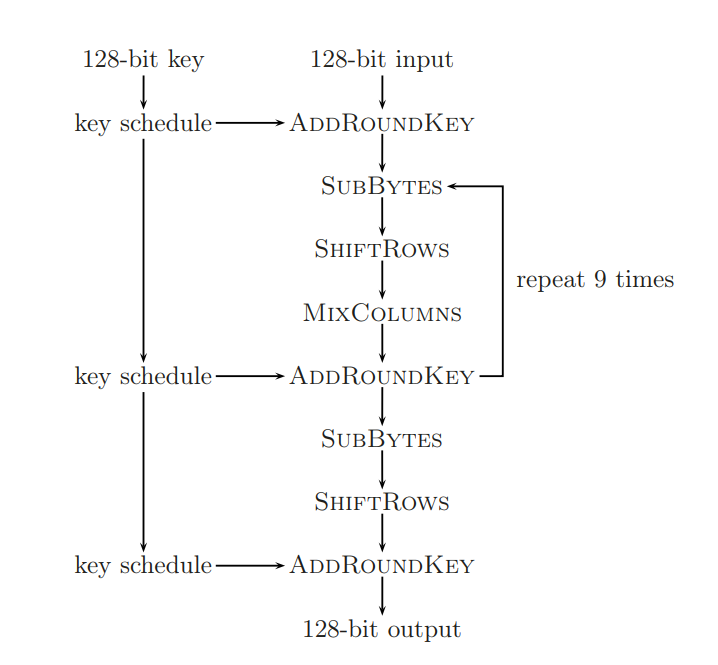
\includegraphics[width=0.7\textwidth, height=0.7\textheight, keepaspectratio]{AES}
        \caption{Rondas de AES-$128$ \cite{cryptoSchool}.}
        \label{fig:1.1}
    \end{figure}
    
    Seguidamente, vamos a proceder a explicar en más detalle las distintas operaciones que constituyen AES. A medida que avancemos en este documento, también exploraremos otros sistemas de cifrado como RSA o Merkle-Hellman, entre otros. No obstante, de la elegante explicación algebraica que se presenta a continuación, destaca la sorprendente eficacia del álgebra en el campo de la criptografía.

    \subsection{Operaciones de AES}

    La unidad básica de procesamiento es el byte, formado por $8$ bits.
    \begin{equation}
        a = (a_{7}, a_{6}, a_{5}, a_{4}, a_{3}, a_{2}, a_{1}, a_{0}) \in \{0, 1\}^{8}
    \end{equation}
    Las operaciones básicas de los bytes son la suma y la multiplicación. Las definimos de la siguiente forma:
    \begin{itemize}
        \item \textbf{Suma}. Sean $a, b, c \in \{0, 1\}^{8}$, la suma de dos bytes es la suma bit a bit módulo $2$:
        \begin{equation}
            c_{i} = (a_{i} + b_{i}) \text{ mod } 2 \text{ , con } i = 0, ... , 7
        \end{equation}
        \begin{ejemplo}
            Por ejemplo, sea $a = (1, 0, 0, 1, 1, 0, 1, 1)$ y $b = (1, 1, 0, 0, 1, 1, 0, 1)$, entonces: 
            \begin{equation}
                c = a + b = (0, 1, 0, 1, 0, 1, 1, 0)
            \end{equation}
        \end{ejemplo}
        \item \textbf{Producto}. Para el producto, consideramos que el byte $a$ está representando el siguiente polinomio:
        \begin{equation}
            a_{7}t^{7} + a_{6}t^{6} + \ldots + a_{1}t + a_{0} \in \mathbb{F}_{2}[t]
        \end{equation}
        De esta forma, el producto $p = a \cdot b$ se calcula multiplicando ambos polinomios, obteniendo un polinomio de grado $14$ como máximo. Aunque ahora tenemos un problema obvio, ya que el resultado obtenido tiene $15$ bits pero la operación debe devolver al final solo $8$. Para solucionar esto, lo que haremos será reducir módulo un polinomio de grado $8$. De hecho, en AES trabajamos en el campo finito $\mathbb{F}_{256}$ definido por el polinomio irreducible:
        \begin{equation}
            m = t^{8} + t^{4} + t^{3} + t + 1 \in \mathbb{F}_{2}[t]
        \end{equation}
        Por tanto, $p$ mod $m \in \mathbb{F}_{2}[t]/(m) = \mathbb{F}_{2^{8}} = \mathbb{F}_{256}$, volviendo de nuevo al grado máximo de $8$ bits que nos da el resultado final del producto:
        \begin{align}
            c = a_{7}t^{7} + a_{6}t^{6} + &a_{5}t^{5} + a_{4}t^{4} + a_{3}t^{3} + a_{2}t^{2} + a_{1}t + a_{0} \in \mathbb{F}_{256} \\
            &\text{con } a_{i} \in \{0, 1\} \text{, } i = 0, ... , 7
        \end{align}
        Veamos un ejemplo que nos clarifique los conceptos vistos.
        \begin{ejemplo}
            Sea $a = (1, 0, 0, 1, 1, 0, 1, 1)$ y $b = (1, 1, 0, 0, 1, 1, 0, 1)$ los mismos valores de antes. Ahora, sin embargo, representan los siguientes polinomios respectivamente:
            \begin{align}
                a = t^{7} + t^{4} + t^{3} + t + 1 \in \mathbb{F}_{2}[t] \\
                b = t^{7} + t^{6} + t^{3} + t^{2} + 1 \in \mathbb{F}_{2}[t]
            \end{align}
            El producto de estos polinomios es:
            \begin{equation}
                p = t^{14} + t^{13} + t^{11} + t^{10} + t^{8} + t^{6} + t^{5} + t^{3} + t^{2} + t + 1 \in \mathbb{F}_{2}[t]
            \end{equation}
            Recordemos que el polinomio irreducible es:
            \begin{equation}
                m = t^{8} + t^{4} + t^{3} + t + 1 \in \mathbb{F}_{2}[t]
            \end{equation}
            A continuación, calculamos $p$ mod $m$, esto es, dividimos $p$ entre $m$ y nos quedamos con el resto, obteniendo:
            \begin{equation}
                p = (t^{6} + t^{5} + t^{3}) \cdot m + (t^{4} + t^{2} + t + 1) \in \mathbb{F}_{2}[t]
            \end{equation}
            Finalmente, fijándonos en el resto, obtenemos que este polinomio es la representación de $c = (0, 0, 0, 1, 0, 1, 1, 1)$.
        \end{ejemplo}
    \end{itemize}

    \subsubsection{SubBytes}

    La operación SubBytes de AES aplica una transformación a cada byte de la matriz $4x4$. Es por ello que el apartado anterior define las dos operaciones principales que vamos a utilizar, la suma y el producto. Estas operaciones las realizamos a partir de dos bytes, obteniendo otro byte como resultado. El problema es que en SubBytes, solo tenemos un byte de entrada. Para solucionar esto, haremos uso de la inversa.

    Como $\mathbb{F}_{256}$ es un cuerpo, todo elemento no nulo $a \in \mathbb{F}^{x}_{256}$ tiene un inverso $a^{-1} \in \mathbb{F}^{x}_{256}$. Este elemento inverso se puede calcular mediante el Algoritmo Extendido de Euclides. Definimos esta función en todo $\mathbb{F}_{256}$ simplemente enviando cero a si mismo:
    \[
    \text{inv(}a\text{)} = 
    \left\{
        \begin{array}{l}
            a^{-1} \text{, si } a \neq 00 \\
            00 \text{, si } a = 00 
        \end{array}
    \right.
    \]
    donde $00 = (0, 0, 0, 0, 0, 0, 0, 0)$. Entendamos lo explicado en el siguiente ejemplo.
    \begin{ejemplo} \cite{cryptoSchool}
        Tomando los valores de los ejemplos vistos previamente, el Algoritmo Extendido de Euclides nos da la siguiente igualdad:
        \begin{equation}
            (t^{7} + t^{3}) \cdot a + (t^{6} + t^{3} + t^{2} + t + 1) \cdot m = 1 \text{, en } \mathbb{F}_{2}[t]
        \end{equation}
        De hecho, como gcd($a,m$) = $1$, entonces:
        \begin{equation}
            \text{inv(}a\text{)} = (1, 0, 0, 0, 1, 0, 0, 0) \text{ en } \mathbb{F}_{256}.
        \end{equation}
    \end{ejemplo}

    AES utiliza una estructura algebraica similar, aunque diferente, sobre los bytes, llamada el anillo $R =  \mathbb{F}_{2}[t]/(t^{8}+1)$. Esta estructura no es un cuerpo, ya que $t^{8}+1 = (t+1)^{8}$ no es irreducible en $\mathbb{F}_{2}[t]$. Por tanto, ahora un byte $a$ representa al elemento:
    \begin{equation}
        a_{7}t^{7} + a_{6}t^{6} + a_{5}t^{5} + a_{4}t^{4} + a_{3}t^{3} + a_{2}t^{2} + a_{1}t + a_{0} \text{ en } R
    \end{equation}
    La suma, nuevamente, es la suma de bits módulo dos (o XOR), por lo que es válido en R. En la multiplicación, también se lleva a cabo el producto de polinomios, para luego reducir su grado tomando módulo con un polinomio de grado $8$, solo que en este caso, este polinomio de reducción es $m = t^{8}+1$. Esta reducción es particularmente sencilla ya que corresponde a dividir la parte superior e inferior del polinomio producto $p$ con tamaño $16$ bits, en dos partes que denominaremos $c_{1}$ y $c_{0}$ respectivamente, de tamaño $8$ bits cada una, para luego sumarlas y obtener el resultado final. Veamos esta idea en un ejemplo que nos resulte claro.

    \begin{ejemplo} 
        Tomando $a = (1, 0, 0, 1, 1, 0, 1, 1)$ y $b = (1, 1, 0, 0, 1, 1, 0, 1)$ los mismos valores previos, realizamos la multiplicación de los polinomios y obtenemos el mismo resultado anterior:
        \begin{equation}
            p = t^{14} + t^{13} + t^{11} + t^{10} + t^{8} + t^{6} + t^{5} + t^{3} + t^{2} + t + 1
        \end{equation}
        Recordemos ahora que el polinomio irreducible es:
        \begin{equation}
            m = t^{8} + 1
        \end{equation}
        Por tanto, aplicando ahora reducción de $p$ módulo $m$, obtendríamos lo siguiente:
        \begin{equation}
            p = (t^{6} + t^{5} + t^{3} + t^{2} + t + 1) \cdot m + t 
        \end{equation}
        Por tanto, el resultado final es $c = (0, 0, 0, 0, 0, 0, 1, 0)$, ya que debemos centrarnos solo en el resto. No obstante, lo particular de este polinomio irreducible es que es más fácil su cálculo, ya que podemos dividir el polinimio $p$ en dos partes, que hemos denominado $c_{1}$ y $c_{0}$. Esta idea se expresa en la siguiente igualdad:
        \begin{equation}
            p = c_{1} \cdot t^{8} + c_{0}
        \end{equation}
        Así, para calcular cada $c_{i}$, debemos dividir del polinomio $p$ con tamaño $16$ bits, en dos mitades con $8$ bits cada una, de tal forma que obtenemos:
        \begin{align}
            c_{1} = (0, 1, 1, 0, 1, 1, 0, 1) \\
            c_{0} = (0, 1, 1, 0, 1, 1, 1, 1)
        \end{align}
        Para finalizar, solo debemos sumar ambas $c_{i}$ usando la suma en $R$ y obtendremos el resultado final $c = (0, 0, 0, 0, 0, 0, 1, 0)$, que coincide con el que habíamos obtenido.
    \end{ejemplo}
    
    Tras haber explicado todo esto, cabe mencionar que en AES, realmente sólo se realiza el producto en $R$ por el polinomio fijo $t_{1}$, y solo se suma el polinomio $t_{0}$. Estos son:
    \begin{align}
        &t_{1} = (0, 0, 0, 1, 1, 1, 1, 1) = t^{4} + t^{3} + t^{2} + t + 1 \\
        &t_{0} = (0, 1, 1, 0, 0, 0, 1, 1) = t^{6} + t^{5} + t + 1 
    \end{align}
    Al ser $t_{1}$ invertible módulo $t^{8} + 1$, la multiplicación por $t_{1}$ corresponde a una transformación lineal invertible sobre $\mathbb{F}_{2}$. Así, para un byte $a$, debemos aplicar:
    \begin{equation}
        c = t_{1} \cdot b + t_{0}
    \end{equation}
    donde $b =$ inv($a$), visto previamente. Esto también puede ser descrito por una transformación lineal de la siguiente forma:
    \begin{equation}
        \begin{bmatrix}
            c_{7} \\
            c_{6} \\
            c_{5} \\
            c_{4} \\
            c_{3} \\
            c_{2} \\
            c_{1} \\
            c_{0} \\
        \end{bmatrix}
        =
        \begin{bmatrix}
            1 & 1 & 1 & 1 & 1 & 0 & 0 & 0 \\
            0 & 1 & 1 & 1 & 1 & 1 & 0 & 0 \\
            0 & 0 & 1 & 1 & 1 & 1 & 1 & 0 \\
            0 & 0 & 0 & 1 & 1 & 1 & 1 & 1 \\
            1 & 0 & 0 & 0 & 1 & 1 & 1 & 1 \\
            1 & 1 & 0 & 0 & 0 & 1 & 1 & 1 \\
            1 & 1 & 1 & 0 & 0 & 0 & 1 & 1 \\
            1 & 1 & 1 & 1 & 0 & 0 & 0 & 1 \\
        \end{bmatrix}
        \cdot
        \begin{bmatrix}
            b_{7} \\
            b_{6} \\
            b_{5} \\
            b_{4} \\
            b_{3} \\
            b_{2} \\
            b_{1} \\
            b_{0} \\
        \end{bmatrix}
        +
        \begin{bmatrix}
            0 \\
            1 \\
            1 \\
            0 \\
            0 \\
            0 \\
            1 \\
            1 \\
        \end{bmatrix}
    \end{equation}

    Finalmente como resumen, SubBytes consiste en aplicar a cada byte $a$ del bloque los siguientes pasos:
    \begin{align}
        &a \leftarrow \text{inv(}a\text{) , en } \mathbb{F}_{256} \\
        &a \leftarrow t_{1} \cdot a \text{ , en } R \\
        &a \leftarrow a + t_{0} \text{ , en } R
    \end{align}
    SubBytes es la única operación no lineal de AES. Como curiosidad, a veces es llamada ``S-box'', en analogía a las funciones no lineales de DES.

    \subsubsection{ShiftRows}
    
    La operación ShiftRows de AES desplaza cada una de las cuatro filas cíclicamente hacia la izquierda en $0$, $1$, $2$ y $3$ posiciones, respectivamente, ya que recordemos que estamos trabajando con AES-$128$.
    \begin{ejemplo}
        De manera genérica, aplicando ShiftRows a nuestra matriz inicial, obtendremos:
        \begin{equation}
            \begin{bmatrix}
                a_{00} & a_{01} & a_{02} & a_{03} \\
                a_{10} & a_{11} & a_{12} & a_{13} \\
                a_{20} & a_{21} & a_{22} & a_{23} \\
                a_{30} & a_{31} & a_{32} & a_{33} \\
            \end{bmatrix}
            \rightarrow
             \begin{bmatrix}
                a_{00} & a_{01} & a_{02} & a_{03} \\
                a_{11} & a_{12} & a_{13} & a_{10} \\
                a_{22} & a_{23} & a_{20} & a_{21} \\
                a_{33} & a_{30} & a_{31} & a_{32} \\
            \end{bmatrix}
        \end{equation}
    \end{ejemplo}

    \subsubsection{MixColumns}

    Como ya hemos mencionado, la operación MixColumns de AES aplica una transformación lineal a cada columna de la matriz $4x4$ de bytes. Para ello, vamos a utilizar una estructura algebraica similar a la explicada en SubBytes. Consideramos cada vector $a = (a_{3}, a_{2}, a_{1}, a_{0})$ de $4$ bytes como un polinomio de grado máximo $3$:
    \begin{equation}
        a_{3} \cdot t^{3} + a_{2} \cdot t^{2} + a_{1} \cdot t + a_{0} \in \mathbb{F}_{256}[t]
    \end{equation}
    Donde la suma corresponde a la suma de bits módulo dos (o XOR) y el producto corresponde al ya explicado, con la diferencia de que el polinomio irreducible en este caso es $t^{4} + 1 \in \mathbb{F}_{256}[t]$. Entonces, ahora trabajamos en el anillo $R = \mathbb{F}_{256}[t]/(t^{4} + 1)$, con $256^{4}$ elementos. Al igual que antes, $t^{4} + 1 = (t + 1)^{4}$ no es irreducible en $\mathbb{F}_{256}[t]$, por lo que $R$ no es un cuerpo. Además, la reducción módulo el polinomio irreducible es también particularmente sencilla, ya que podemos dividir el polinimio producto $p$ en dos partes, que denominamos $c_{0}$, $c_{1} \in \mathbb{F}_{256}[t]$, con grado máximo $3$, como se muestra en la siguiente igualdad:
    \begin{equation}
        p = c_{1} \cdot t^{4} + c_{0}
    \end{equation}
    De esta forma, para calcular el producto solo debemos sumar ambas $c_{i}$ usando la suma en $R$ para obtener el resultado final.

    Sin embargo podemos verlo de otra forma, ya que el producto puede ser descrito como un vector de $4$ bytes $b = (b_{3}, b_{2}, b_{1}, b_{0})$, dado por el siguiente producto matriz por vector:
    \begin{equation}
        \begin{bmatrix}
                b_{3} \\
                b_{2} \\
                b_{1} \\
                b_{0} \\
        \end{bmatrix}
        =
        \begin{bmatrix}
                02 & 01 & 01 & 03 \\
                03 & 02 & 01 & 01 \\
                01 & 03 & 02 & 01 \\
                01 & 01 & 03 & 02 \\
        \end{bmatrix}
        \cdot
        \begin{bmatrix}
                a_{3} \\
                a_{2} \\
                a_{1} \\
                a_{0} \\
        \end{bmatrix}
    \end{equation}
    Donde las operaciones entre bytes individuales son las de $\mathbb{F}_{256} = \mathbb{F}_{2}[t]/(t^{4} + 1)$, es decir, las explicadas arriba. Veamos a continuación un ejemplo de MixColumns.

    \begin{ejemplo} \cite{cryptoSchool}
        Sea $a = (\text{A}0, 80, 01, 02)$ una columna de la matriz de bytes, aplicamos MixColumns de la siguiente forma:
        \begin{equation}
            \begin{bmatrix}
                b_{3} \\
                b_{2} \\
                b_{1} \\
                b_{0} \\
            \end{bmatrix}
            = 
            \begin{bmatrix}
                02 & 01 & 01 & 03 \\
                03 & 02 & 01 & 01 \\
                01 & 03 & 02 & 01 \\
                01 & 01 & 03 & 02 \\
            \end{bmatrix}
            \cdot
            \begin{bmatrix}
                \text{A}0 \\
                80 \\
                01 \\
                02 \\
            \end{bmatrix}
        \end{equation}
        Así, 
        \begin{align}
            b_{3} &= 02 \cdot \text{A}0 + 01 \cdot 80 + 01 \cdot 01 + 03 \cdot 02 \\
            &= t \cdot (t^{7} + t^{5}) + 1 \cdot t^{7} + 1 \cdot 1 + (t + 1) \cdot t \\
            &= t^{8} + t^{7} + t^{6} + t^{2} + t + 1 \\
            &= t^{7} + t^{6} + t^{4} + t^{3} + t^{2} \\
            &= (1, 1, 0, 1, 1, 1, 0, 0) \\
            &= \text{FC en } \mathbb{F}_{256}
        \end{align}
        Donde hemos tenido en cuenta que $t^{8} = t^{4} + t^{3} + t + 1$ en $\mathbb{F}_{256}$. Analogamente,
        \begin{align}
            b_{2} &= 03 \cdot \text{A}0 + 02 \cdot 80 + 01 \cdot 01 + 01 \cdot 02 \\
            &= (t + 1) \cdot (t^{7} + t^{5}) + t \cdot t^{7} + 1 \cdot 1 + 1 \cdot t \\
            &= t^{7} + t^{6} + t^{5} + t + 1 \\
            &= (1, 1, 1, 0, 0, 0, 1, 1) \\
            &= \text{E}3 \text{ en } \mathbb{F}_{256}
        \end{align}
        \begin{align}
            b_{1} &= 01 \cdot \text{A}0 + 03 \cdot 80 + 02 \cdot 01 + 01 \cdot 02 \\
            &= 1 \cdot (t^{7} + t^{5}) + (t + 1) \cdot t^{7} + t \cdot 1 + 1 \cdot t \\
            &= t^{5} + t^{4} + t^{3} + t + 1 \\
            &= (0, 0, 1, 1, 1, 0, 1, 1) \\
            &= 3\text{B} \text{ en } \mathbb{F}_{256}
        \end{align}
        \begin{align}
            b_{0} &= 01 \cdot \text{A}0 + 01 \cdot 80 + 03 \cdot 01 + 02 \cdot 02 \\
            &= 1 \cdot (t^{7} + t^{5}) + 1 \cdot t^{7} + (t + 1) \cdot 1 + t \cdot t \\
            &= t^{5} + t^{2} + t + 1 \\
            &= (0, 0, 1, 0, 0, 1, 1, 1) \\
            &= 27 \text{ en } \mathbb{F}_{256}
        \end{align}
        Finalmente,
        \begin{equation}
            b = 
            \begin{bmatrix}
                b_{3} \\
                b_{2} \\
                b_{1} \\
                b_{0}
            \end{bmatrix}
            =
            \begin{bmatrix}
                \text{FC} \\
                \text{E}3 \\
                3\text{B} \\
                27 \\
            \end{bmatrix}
        \end{equation}
        Obteniendo así el resultado final de aplicar MixColumns al vector columna $a$.
    \end{ejemplo}

    \subsubsection{AddRoundKey}

    La operación AddRoundKey de AES suma bit a bit un bloque de $128$ bits con una clave de ronda de su mismo tamaño. Como ya hemos explicado, AES permite claves de $128$, $192$ o $256$ bits. Estas claves corresponden a $l_{k}$ palabras de $32$ bits, con $l_{k} = 4, 6$ o $8$. Además, el número de rondas tras la inical, denominado $l_{r}$, se muestra en la siguiente tabla:

    \begin{figure}[H]
        \centering
        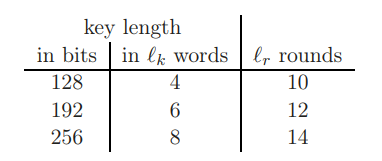
\includegraphics[width=0.5\textwidth, height=0.5\textheight, keepaspectratio]{Claves_de_AES}
        \caption{Número de palabras $l_{k}$ y de rondas $l_{r}$ de AES \cite{cryptoSchool}.}
        \label{fig:1.2}
    \end{figure}
    
    En realidad, cada palabra tiene la forma de un vector columna, simplemente $l_{k}$ indica cuantas filas componen a ese vector. En esta operación buscamos en cada ronda generar una clave de ronda, que será un vector con tantas componentes como rondas $l_{k}$ haya, más una para la ronda inicial. Por tanto, se requiere un total de $l_{k} \cdot (l_{r} + 1)$ claves de ronda.

    \begin{ejemplo}
        Por ejemplo, para una llave de $256$ bits, los mensajes consisten en $8$ palabras de $4$ bytes cada una, equivalentemente, $8$ palabras de $32$ bits cada una. Esto lo sabemos ya que a partir de la figura \ref{fig:1.2}, la clave está formada por $l_{k} = 8$ palabras del tipo $K_{0}, ... , K_{7}$. Además, sabemos que el número de rondas es $l_{r} = 14$, por lo que necesitaremos una clave extendida de $l_{k}(l_{r} + 1) = 8 \cdot (14 + 1) = 120$ palabras.
    \end{ejemplo}

    Procedemos a continuación a explicar esta operación para AES-$128$, es decir, tomando $l_{k} = 4$ y $l_{r} = 10$. La clave secreta $K$ está formada por las cuatro primeras palabras de $32$ bits $E_{0}, E_{1}, E_{2}$ y $E_{3}$ de la clave extendida $E_{0}, ... , E_{4(l_{r}+1)-1}$, que consta de $4(l_{r} + 1)$ palabras de $32$ bits. El resto se generarán a partir de las que ya tenemos. Así, nuestras claves de ronda consistirán en bloques de $4$ palabras consecutivas de la clave extendida. La forma de calcular el resto de palabras es la siguiente:
    \begin{equation}
        E_{i} = E_{i-1} + E_{i-4} \text{ , con } i \geq 4
    \end{equation}
    Esto no es más que la suma en $\mathbb{Z}_{2}^{32}$, en otras palabras, la suma de bits módulo dos o XOR, vista anteriormente. 
    
    No obstante, si $i$ es múltiplo de $4$, se aplica primero una transformación al elemento $E_{i-1}$ tal que sus elementos $(a_{0}, a_{1}, a_{2}, a_{3})$ se desplazan hacia la derecha cíclicamente, obteniendo $(a_{3}, a_{0}, a_{1}, a_{2})$. Es más, si tomamos cada palabra como un elemento $a$ de $S = \mathbb{F}_{256}[t]/(t^{4} + 1)$, consiste simplemente en multiplicar por $t^{3}$ en $S$. Despues, se aplica SubBytes a cada byte individualmente, y se añade una constante $c_{i/4}$, definida de esta forma:
    \begin{equation}
        c_{j} = (0, 0, 0, t^{j-1}) = t^{j-1} \text{ en } S
    \end{equation}
    Decimos que es una constante porque, tomandola como un elemento de $S$, tiene la forma $a_{3}t^{3} + a_{2}t^{2} + a_{1}t + a_{0}$, con $a_{3} = a_{2} = a_{1} = 0$.

    Por último, en el caso en que trabajemos con AES-$256$ y por tanto $l_k = 8$ y $l_r = 14$, se aplica otra transformación. Consiste en que $E_{i-1}$, se reemplaza por SubBytes($E_{i-1}$), si $i$ mod $8$ = $4$. Poniendo toda esta información en común, obtenemos este algoritmo explicativo:

    \begin{algorithm}[H]
        \caption{Algoritmo de clave extendida de AES}
        \textbf{Input:} Clave $K_{0}, ..., K_{l_{k}-1}$ formada por $l_{k}$ palabras, donde cada $K_{i}$ tiene $4$ bytes.\\
        \textbf{Output:} Clave extendida $E_{0}, ... , E_{l_{k}(l_{r}+1)-1}$ formada por $l_{k}(l_{r}+1)$ palabras, donde cada $E_{i}$ tiene $4$ bytes.
        \bigskip
        \begin{algorithmic}[1]
            \For{$i$ from $0$ to $l_{k}-1$}
            \State $E_{i} = K_{i}$
            \EndFor
            \For{$i$ from $l_{k}$ to $l_{k} \cdot (l_{r}+1)$}
            \State $L = E_{i-1}$
            \If{$l_{k}$ divides $i$}
            \State $c = (0, 0, 0, t^{(i/l_{k}) - 1})$
            \State $L$ = SubBytes$(s^{3} \cdot L) + c$
            \EndIf
            \If{$l_{k} == 8$ and $i$ mod $8$ == $4$}
            \State $L$ = SubBytes($L$)
            \EndIf
            \State $E_{i} = E_{i - l_{k}} + L$
            \EndFor
        \end{algorithmic}
    \end{algorithm}

    Una vez hemos descrito todas las operaciones de AES para una ronda, solo nos hace falta repetirlas en el orden y el número de veces que indica la figura \ref{fig:1.1} del principio. Aunque debemos tener en cuenta que dependiendo de qué AES estemos utilizando, el número de rondas será distinto. Con esto, damos por concluida nuestra descripción general del cifrado de AES.

    \subsection{Comentarios sobre AES}
    
    Primeramente, debemos saber que AES evolucionó a partir de los cifrados por bloques desarrollados por sus diseñadores, previos a Rijndael. Tales como ``SHARK'', desarrollado por Vincent Rijmen; y ``Square'', desarrollado por Joan Daemen. Así, su filosofía de diseño perseguía un alto nivel de rendimiento y resistencia contra el criptoanálisis lineal y diferencial.

    Como ejemplos, destacamos que para SubBytes, fué sugerida la idea de utilizar la operación de inversión, y que el módulo $m$ es el primero de los $30$ polinomios irreducibles de la Tabla C del capítulo $10$ de ``Finite Fields'' de Rudolf Lidl \& Harald Niederreiter \cite{artLidl}. MixColumns además se basa en matrices en las que cada submatriz cuadrada es no singular, una noción explicada en el teorema $8$ del capítulo $11$ de ``The theory of error-correcting codes'' de MacWilliams \& Sloane \cite{artMacSlo}.

    Asimismo, la omisión de MixColumns en la última ronda es bastante común, ya que no disminuye la seguridad (porque los bits del texto cifrado sólo se permutan de una forma públicamente conocida), pero permite el descifrado con una estructura similar.
    
    En cuanto a su rendimiento, tal y como se exige en la competición de AES, el algoritmo es rápido en una gran variedad de plataformas. Las implementaciones de software pueden alcanzar más de $12$ GB/seg. Aun así, si tenemos como objetivo realizar una implementación de software, debemos saber que generalmente es ventajoso sustituir los cálculos por consultas de tablas. Utilizando una tabla de $4$ KB, una ronda de AES puede ejecutarse con $16$ búsquedas en la tabla y $16$ XOR de $32$ bits.

    Por otro lado, en cuanto a su seguridad, sí que es cierto que algunos criptógrafos muestran preocupación, ya que sienten que el margen entre el número de rondas especificado en el cifrador y los mejores ataques conocidos es muy pequeño. Además, se especula con ataques teóricos, como por ejemplo el denominado ``Ataque XSL'', que teóricamente muestra una potencial debilidad en el algoritmo AES. Sin embargo, tanto los expertos como las instituciones de normalización más relevantes consideran que AES es seguro.

    \newpage
 
    \section{Criptografía simétrica vs asimétrica} \label{sec:1.3}

    Hasta ahora, solo hemos trabajado con AES, un criptosistema de tipo simétrico. Este tipo de criptosistemas se caracterizan porque la misma clave que se utiliza para cifrar el mensaje, es la que se usa para descifrarlo. Al igual que AES, todos los cifrados previos a $1970$ eran de este tipo. 
    
    Sin embargo, Diffie \& Hellman \cite{artDH} hicieron una propuesta revolucionaria en $1976$ publicando su libro ``New directions in cryptography'', en el que presentaron un algoritmo que demostró que la criptografía asimétrica era posible. En él, proponen un nuevo método de comunicación donde cada usuario posee dos claves, una privada y una pública. Digamos que Alice quiere enviar un mensaje a Bob. Entonces Alice debe utilizar la clave pública de Bob para encriptar el mensaje que le mandará. Gracias a la clave secreta, Bob puede fácilmente desencriptar el mensaje de Alice, pero sin ella, nadie debería poder.
    
    Con la llegada de este nuevo tipo de criptosistemas, se comenzó a estudiar si estos eran mejores o peores que los ya conocidos criptosistemas simétricos. Pero como en todo, se encontraron ventajas y desventajas en cada uno de ellos. 
    
    Por un lado, la ventaja de los criptosistemas asimétricos radica en que no necesitan un cambio de clave. Por otro, los criptosistemas simétricos tienen ventaja de velocidad, ya que como hemos mencionado, AES puede alcanzar $12$ GB/seg. Otra ventaja de estos últimos es la autenticación, puesto que en los criptosistemas asimétricos debemos tomar medidas para garantizar esta característica. 

    Actualmente, la realidad es que no existe una rivalidad entre criptografía ``Simétrica vs Asimétrica''. Por lo general, se utiliza un método asimétrico para compartir las claves necesarias y así, posteriormente, poder aplicar un criptosistema simétrico permitiendo comunicación de mayor rendimiento. 
    
    Veamos a continuación dos ejemplos de criptosistemas asimétricos para conocerlos un poco más a fondo, comenzando por el famoso criptosistema RSA.

    \section{Criptosistema RSA}

    Basándose en el primer modelo abstracto de criptosistema de clave pública sugerido por Diffie \& Hellman en $1976$, Rivest, Shamir \& Adleman crearon su propio criptosistema asimétrico en $1977$ llamado ``Rivest-Shamir-Adleman cryptosystem'', o más conocido como RSA.

    Continuemos con la notación de nombres utilizada hasta ahora. En nuestro escenario, Alice quiere enviar un mensaje a Bob, que sólo él sea capaz de leerlo. Para ello, Bob genera dos claves: una clave pública $pk$ y una clave privada $sk$. Cualquiera puede conocer la clave pública $pk$. Puede estar expuesta en una base de datos o en internet, mismamente. Sin embargo, la clave privada $sk$ sí que debe ser guardada por Bob en secreto. De esta forma, Alice usará la clave pública $pk$ para encriptar su mensaje y Bob usará su clave privada $sk$ para descifrarla.

    En los criptosistemas simétricos, el cifrado y descrifrado se realiza esencialmente con la misma clave, pero aquí, $pk$ y $sk$ son claves completamente distintas. De hecho, deben cumplir algunas propiedades como que $sk$ no debe ser computable facilmente a partir de $pk$; y deben verificar que $dec_{sk}(enc_{pk}(x)) = dec_{pk}(enc_{sk}(x)) = x$, siendo $x$ el mensaje original.

    El mensaje puede ser una imagen, un texto, un video, o incluso un programa. Pero vamos a suponer que ya ha sido convertido a un string binario (posiblemente muy largo), que será nuestra forma de comunicación estándar. Esta conversión dependerá del tipo de dato que se trate, como por ejemplo, la manera más común de enviar un texto es haciendo uso de la codificación ASCII o ASCII extendida, en letras de $7$ u $8$ bits, respectivamente. Aunque en la práctica, RSA se utiliza para enviar una clave secreta y así establecer un criptosistema simétrico; o para garantizar autenticidad mediante firmas digitales. 

    En nuestro escenario, estamos suponiendo que Alice quiere enviarle un mensaje a Bob. Para ello, Alice debe tener en cuenta el valor $n$, denominado \textit{parámetro de seguridad}, ya que debe dividir el mensaje $x$ en bloques de tamaño $n-1$ bits y enviar cada bloque por separado. Por tanto, vamos a explicar como se envía un bloque de $n-1$ bits usando el criptosistema de RSA.

    En primer lugar, Bob debe elegir dos valores primos $p$ y $q$ aleatorios, con $\frac{n}{2}$ bits cada uno. Así, su producto $N = p \cdot q$ tendrá $n$ bits. Además, Bob debe elegir un número entero $e$ aleatorio, tal que $1 \leq e < N$ y gcd($e, (p-1)(q - 1)) = 1$, es decir, $e$ y el producto $(p-1) \cdot (q-1)$ sean coprimos. Así, la clave pública de Bob es $pk = (N, e)$. 

    A continuación, a partir del mensaje $x$, Alice envía a Bob el mensaje encriptado $y = x^{e}$ en $\mathbb{Z}_{n}$, esto es, el resto de dividir $x^{e}$ entre $N$. La magia es que Bob ahora puede recuperar el mensaje de Alice $x$ con la ayuda de su información secreta relativa a $(p,q)$. El algoritmo es el siguiente:

    \begin{algorithm}[H]
        \caption{Algoritmo de generación de claves de RSA}
        \textbf{Input:} Parámetro de seguridad $n$.\\
        \textbf{Output:} Clave privada $sk$ y clave pública $pk$.
        \bigskip
        \begin{algorithmic}[1]
            \State Elegir los valores primos $p$, $q$ tal que $2^{(n-1)/2} < p$ y $q < 2^{n/2}$.
            \State Calcular $N = p \cdot q$ con $n$ bits y $L = (p - 1) \cdot (q - 1) = \phi(p) \cdot \phi(q) = \phi(N)$, es decir, la función de Euler aplicada a $N$.
            \State Escoger $e$ de manera uniformemente aleatoria del conjunto $\{2, ... , L-2\}$, tal que sea coprimo con $L$. Así $e \in \mathbb{Z}_{L}$.
            \State Calcular el inverso $d$ de $e$ en $\mathbb{Z}_{L}$. Así $d \in \mathbb{Z}_{L}$.
            \State Revelar la clave pública $pk = (N, e)$ y esconder la clave privada $sk = (N, d)$.
        \end{algorithmic}
    \end{algorithm}

    \begin{algorithm}[H]
        \caption{Algoritmo de cifrado de RSA}
        \textbf{Input:} Mensaje $x \in \mathbb{Z}_{N}$ y clave pública $pk = (N, e)$.\\
        \textbf{Output:} Mensaje cifrado $y = enc_{pk}(x) \in \mathbb{Z}_{N}$.
        \bigskip
        \begin{algorithmic}[1]
            \State Aplicar la transformación $y = x^{e}$ en $\mathbb{Z}_{N}$.
            \State Devolver el mensaje cifrado $y = enc_{pk}(x)$.
        \end{algorithmic}
    \end{algorithm}
    
    \begin{algorithm}[H]
        \caption{Algoritmo de descifrado de RSA}
        \textbf{Input:} Mensaje cifrado $y \in \mathbb{Z}_{N}$ y clave privada $sk = (N, d)$.\\
        \textbf{Output:} Mensaje original $x = dec_{sk}(y) \in \mathbb{Z}_{N}$.
        \bigskip
        \begin{algorithmic}[1]
            \State Aplicar la transformación $x = y^{d}$ en $\mathbb{Z}_{N}$.
            \State Devolver el mensaje original $x = dec_{sk}(y)$.
        \end{algorithmic}
    \end{algorithm}
    
    \begin{ejemplo} \label{ej: 1.11}
        Veamos un ejemplo tomando $n = 6$. Si en este caso comprobamos las condiciones de manera literal, debemos escoger números primos entre $6$ y $7$, pero al ser valores tan pequeños, tomaremos la libertad de ser un poco más liberales y escogeremos $p = 7$ y $q = 11$. Así, $N = 77$ y $L = 60$. Tomando $e = 17$ y aplicando el Algoritmo Extendido de Euclides, obtenemos que $d = e^{-1} = 53$ en $\mathbb{Z}_{60}$. De esta forma, Bob ya puede publicar su clave pública $pk = (77, 17)$ y guardar su clave privada $sk = (77, 53)$.

        Posteriormente, Alice quiere mandarle un mensaje a Bob, pongamos $x = 10 = (00001010)$. Entonces Alice debe cifrar el mensaje $y = x^{e} = 10^{17}$ en $\mathbb{Z}_{77}$. La forma intuitiva para calcular esto sería computar $10^{17}$ y aplicarle el módulo $77$. Pero esto tiene un problema, y es que para valores reales de $n$, $x^{e}$ puede superar el número de partículas en el universo. Sin embargo, hay una forma más sencilla de calcularlo. La idea es descomponer el valor en sus potencias de dos y aplicar módulo tras cada operación para no dejar que el valor se dispare. Veamoslo:
        \begin{align}
            \text{Ya q} & \text{ue }(17)_{10} = (10001)_{2} \Rightarrow 10^{17} = 10^{2^{0}+2^{4}} = 10 \cdot 10^{16} \\
            \text{Calc} & \text{ulamos} \text{ así las potencias de $10$ mod $77$:} \\
            &10 \text{ mod } 77 = 10 \\
            &10^{2} \text{ mod } 77 = 10 \cdot 10 \text{ mod } 77 = 23 \\
            &10^{4} \text{ mod } 77 = 10^{2} \cdot 10^{2} \text{ mod } 77 = 23^{2} \text{ mod } 77 = 67 \\
            &10^{8} \text{ mod } 77 = 10^{4} \cdot 10^{4} \text{ mod } 77 = 67^{2} \text{ mod } 77 = 23 \\
            &10^{16} \text{ mod } 77 = 10^{8} \cdot 10^{8} \text{ mod } 77 = 23^{2} \text{ mod } 77 = 67 \\
            \text{Por } & \text{tanto,} \\
            &10^{17} \text{ mod } 77 = 10 \cdot 10^{16} \text{ mod } 77 = 10 \cdot 67 \text{ mod } 77 = 54
        \end{align}
        Ahora, Alice ya puede enviar su mensaje cifrado $y = enc_{pk}(10) = 54$ a Bob. Por tanto, Bob debe descifrar el mensaje recibido, y para ello, debe usar de manera análoga la descomposición binaria de $53$ (que es el valor de su clave secereta $sk$) para descifrar el mensaje en $\mathbb{Z}_{77}$. De esta forma, $dec_{sk}(54) = x = 54^{53} = 10$ en $\mathbb{Z}_{77}$. De hecho, ese es el mensaje original que Alice quería hacerle llegar a Bob.
    \end{ejemplo}
    
    \begin{observacion}
        Tal y como ya hemos mencionado antes, debemos dejar claro que los valores tomados en este ejemplo son simplemente para esclarecer las ideas del método propuesto, ya que con objetivos prácticos reales, es recomendable que el valor del parámetro de seguridad sea mayor a $n = 3000$.
    \end{observacion}

    \section{Intercambio de claves Diffie-Hellman}

    Para los criptosistemas simétricos como AES, se debe elegir una clave secreta y compartirla entre todos las partes autorizadas. En la práctica, este acuerdo plantea una gran dificultad en este tipo de criptosistemas. Para ilustrar esto, comenzaremos esta sección con un ejemplo histórico.

    Durante la Primera Guerra Mundial, los alemanes quedaron aislados de sus embajadas en el extranjero. Surgieron las sospechas de que sus antiguos códigos de comunicación estaban rotos y enviaron un código nuevo a México y a Washington en un submarino. Sin embargo, esta clave no pudo ser entregada con éxito a México. A pesar de esto, un mensaje secreto de gran importancia llegó sin problemas a Washington utilizando el nuevo código, aunque, posteriormente tuvo que ser retransmitido a México en el código antiguo, el cual fue descifrado. La implementación en su momento de un método público y seguro para el intercambio de claves secretas podría haber evitado esta situación.

    Por tanto, la pregunta es la siguiente: ¿Pueden dos usuarios ponerse de acuerdo sobre una clave secreta compartida (para un criptosistema simétrico) mientras se ven obligados a utilizar un canal inseguro? La sorprendente respuesta es que sí es posible. Obviamente, ninguno puede enviar directamente la clave secreta ya que el canal es inseguro. En lugar de eso, cada usuario debe enviar una versión enmascarada de la clave, a partir de la cual el otro usuario pueda obtenerla, pero un espía no pueda.

    Diffie y Hellman proponen el uso de un número primo $p$, y a partir de él, trabajar con valores que no sean divisibles por $p$ y las propiedades de su producto. Estos valores forman el grupo $\mathbb{Z}_{p}^{x}$ de unidades módulo $p$. En total hay $p - 1$ elementos y el producto de dos de ellos tampoco es divisible por $p$. Además, todos los elementos tienen inverso multiplicativo, que se puede calcular haciendo uso del Algoritmo Extendido de Euclides. Asimismo, este grupo $G = \mathbb{Z}_{p}^{x}$ es \textit{cíclico}, esto es, que existe un elemento $g \in G$, llamado \textit{generador}, cuyas potencias generan todos los elementos de $G = \{g^{0} = 1, g, g^{2}, ... , g^{p-2}\} = \langle g \rangle$. El \textit{orden} del grupo, es decir, el número de elementos de $G$, lo denotaremos como $d$. Aparece ahora un parámetro de seguridad global $n$, que indica el tamaño de $d$ en bits. Así, los elementos de $G$ pueden representarse por cadenas de $n$ bits.

    Un requisito importante es que la representación de $G$ pueda ser expresada utilizando una cantidad de bits que crezca de manera polinómica respecto al valor $n$. Otro requisito, es que las operaciones del grupo puedan transformarse en las representaciones de los elementos de $G$, con una cantidad de operaciones que aumente de manera polinómica respecto a $n$. En general, estos dos requisitos se cumplen de manera clara.

    Algunos ejemplos de $G$ son los siguientes:
    \begin{itemize}
        \item El grupo multiplicativo $G = \mathbb{Z}_{p}^{x}$ de unidades módulo $p$.
        \item El grupo multiplicativo $G = \mathbb{F}_{q}^{x}$ de un cuerpo finito $\mathbb{F}_{q}$.
        \item Grupos cíclicos de curvas elípticas sobre cuerpos finitos.
    \end{itemize}
    
    \begin{ejemplo} \cite{cryptoSchool}
        Sea $G = \mathbb{Z}_{2579}^{x}$ el grupo multiplicativo de unidades módulo $p = 2579$. Como $d = \phi(2579) = 2578 = 2 \cdot 1289$, con $2$ y $1289$ primos, y $2^{2} = 4$ y $2^{1289} = -1$ en $\mathbb{Z}_{2579}^{x}$, ambos distintos de $1$, concluimos que $g = 2 \in G$ es el generador de $G$. Una descripción de $G$ equivale a unos bits diciendo: ``$G$ es de la forma $\mathbb{Z}_{p}^{x}$''. Entonces, $G$ es identificado como el conjunto $\{0, ... , p-1\}$ y la representación binaria de los enteros proporciona la representación de los elementos de $G$. En este ejemplo, tomando $n = 12$, ciertas herramientas para aritmética eficiente muestran que las operaciones de grupo pueden realizarse con coste cuadrático, y por tanto, polinómico en $n$.
    \end{ejemplo}

    Procedemos a describir el intercambio de claves de Diffie-Hellman basándonos en la siguiente representación gráfica.
    
    \begin{figure}[H]
        \centering
        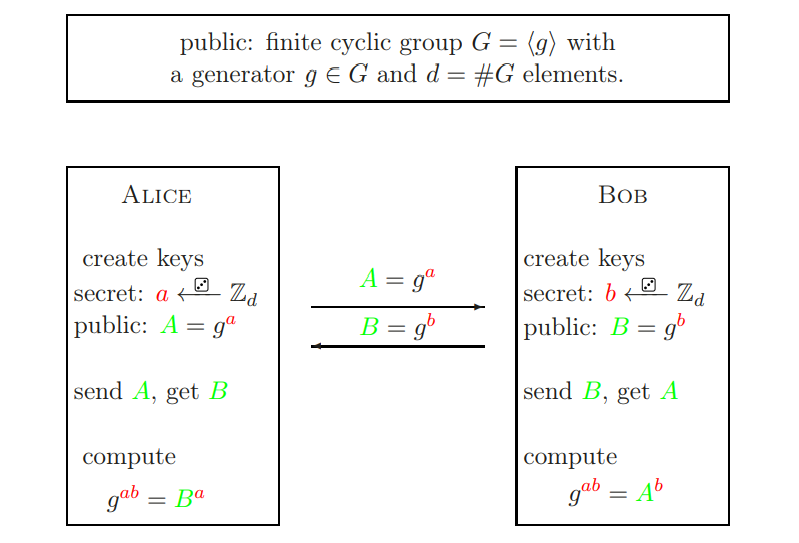
\includegraphics[width=0.8\textwidth, height=0.8\textheight, keepaspectratio]{RepresentacionDH}
        \caption{Esquema del intercambio de claves Diffie-Hellman \cite{cryptoSchool}.}
    \end{figure}

    En primer lugar, Alice y Bob deben elegir de forma independiente una clave secreta aleatoria $a$ y $b \in \mathbb{Z}_{d}$. A continuación, ambos publican sus claves públicas $A = g^{a}$ y $B = g^{b}$, respectivamente. Ahora, ambos pueden calcular, tal vez para su uso en un criptosistema de clave simétrica, la clave secreta compartida $g^{ab}$:
    \begin{equation}
        g^{ab} = B^{a} = A^{b}
    \end{equation}
    ya que
    \begin{equation}
        B^{a} = (g^{b})^{a} = g^{ba} = g^{ab} = (g^{a})^{b} = A^{b}
    \end{equation}
    
    El algoritmo es el siguiente:
 
    \begin{algorithm}[H]
        \caption{Intercambio de claves Diffie-Hellman}
        \textbf{Input:} Parámetro de seguridad $n$.\\
        \textbf{Output:} $G, g, d$ explicadas y clave secreta compartida $k_{B} = k_{A} = g^{ab}$.
        \bigskip
        \begin{algorithmic}[1]
            \State Describir un grupo cíclico finito $G = \langle g \rangle$, siendo $g$ su generador y con $d = \#G$ elementos, donde $d$ es un entero de $n$ bits.
            \State Alice elige su clave secreta $sk = a \in \mathbb{Z}_{d}$, y publica su clave pública $pk = A = g^{a} \in G$.
            \State Bob elige su clave secreta $sk = b \in \mathbb{Z}_{d}$, y publica su clave pública $pk = B = g^{b} \in G$.
            \State Alice y Bob intercambian sus claves públicas $A$ y $B$.
            \State Alice obtiene su clave secreta compartida $k_{A} = B^{a}$ en $G$.
            \State Bob obtiene su clave secreta compartida $k_{B} = A^{b}$ en $G$.
            \State Alice y Bob tienen ahora sus claves secretas compartidas $k_{B} = k_{A}$.
        \end{algorithmic}
    \end{algorithm}

    \begin{ejemplo} \cite{cryptoSchool}
        Continuamos con el ejemplo tratado anteriormente. Podemos así seguir con exactitud los pasos vistos en el algoritmo de intercambio de claves:
        \begin{algorithmic}[1]
            \State Recordemos que estábamos trabajando con $G = \mathbb{Z}_{2579}^{x}$ y cuyo generador es $g = 2 \in G$.
            \State Alice elige su clave secreta $sk = a = 765 \in \mathbb{Z}_{d}$, y publica su clave pública $pk = A = g^{a} = 2^{765} = 949 \in G$.
            \State Bob elige su clave secreta $sk = b = 853 \in \mathbb{Z}_{d}$, y publica su clave pública $pk = B = g^{b} = 2^{853} = 435 \in G$.
            \State Alice y Bob intercambian sus claves públicas $A = 949$ y $B = 435$.
            \State Alice obtiene su clave secreta compartida $k_{A} = B^{a} = 435^{765} = 2424 \in G$.
            \State Bob obtiene su clave secreta compartida $k_{B} = A^{b} = 949^{853} = 2424 \in G$.
            \State Alice y Bob tienen ahora sus claves secretas compartidas $k_{B} = k_{A} = 2424 \in G$.
        \end{algorithmic}
    \end{ejemplo}

    \begin{observacion}
        Como ya hemos mencionado, el método es correcto, en cuanto a que tanto Bob como Alice obtienen la misma clave secreta compartida que les permite generar un cifrado simétrico para comunicarse, entre otras cosas. Por otro lado, en cuanto a eficiencia, la operación más costosa es la exponenciación en $G$, pero justo en el apartado anterior de RSA explicamos una forma de realizar esta operación de manera mucho más eficiente, específicamente en el ejemplo \ref{ej: 1.11}. Por último, el principal problema que tiene este método en cuanto a seguridad, es el ataque conocido como \textit{man-in-the-middle} (MITM). En nuestro caso, este ataque consiste en que Eva se hace pasar por Alice cuando habla con Bob y por Bob cuando intercambia datos con Alice. Ambas partes creen que al otro lado tienen a la pareja legítima, pero Eva puede actuar de forma maliciosa generando su propia parte de la clave compartida utilizada. Para solucionar esto, pueden simplemente comparar si las claves secretas compartidas son idénticas. Si no lo son, pueden estar seguros de que alguien ha estado interfiriendo en su comunicación.
    \end{observacion}

    Para finalizar, debemos destacar que en la actualidad, el protocolo Diffie-Hellman se emplea en situaciones prácticas ampliamente reconocidas. Un ejemplo de su uso es el protocolo de mensajería instantánea conocido como \textit{Off-the-Record Messaging} (OTR). Además, se utiliza en la red de anonimato denominada \textit{Tor}, donde el protocolo Diffie-Hellman se implementa sobre una conexión TLS previamente establecida en una capa inferior. Esta implementación se utiliza para generar claves de sesión entre el cliente y los nodos de enrutamiento de la red, y estas claves se emplean para cifrar las capas de cebolla de los paquetes que circulan a través de la red.
    
\endinput
\chapter{Problema de la mochila} \label{ch:segundo-capitulo}

    En este capítulo vamos a explicar todos los conceptos necesarios para entender el problema de la mochila, pilar de este trabajo y cuestión que trataremos en capítulos posteriores, ya que será la base del criptosistema en el que nos centraremos. Las principales fuentes bibliográficas han sido \cite{probMil}, \cite{defPM}, \cite{theoryComp} y \cite{MTformal}.

    \section{Los siete problemas del milenio}

    Los problemas del milenio son un conjunto de siete enigmas matemáticos que desafían a los científicos desde su formulación en el año $2000$ por el Clay Mathematics Institute. Se hizo como un llamado a resolver siete de los problemas matemáticos más complejos de toda la historia. Para motivar más esta búsqueda, se anunció además que la resolución de cada uno de estos problemas sería premiada con una suma de un millón de dólares. Hasta el día de hoy, sólo uno de estos problemas ha sido resuelto, la Conjetura de Poincaré. 

    A continuación se enumeran los problemas del milenio acompañados de una breve descripción de cada uno \cite{probMil}:

    \begin{enumerate}
        \item \textbf{La conjetura de Hodge}:  Es un problema relacionado con la geometría y la topología algebraica. Se centra en entender la estructura de ciertos espacios matemáticos que surgen al estudiar variedades algebraicas y sus propiedades geométricas. Resolver esta conjetura permitiría un mayor entendimiento de la relación entre el álgebra y la geometría.
        
        \item \textbf{La conjetura de Poincaré}: Plantea que la esfera cuatridimensional ($3$-esfera) es la única variedad compacta cuatridimensional en la que todo lazo ($1$-esfera) se puede deformar en un punto. Este es el único problema que ha sido resuelto hasta el momento.
        
        \item \textbf{La hipótesis de Riemann}: Propone que todos los ceros no triviales de la función zeta de Riemann tienen parte real $\frac{1}{2}$. Resolverla implicaría grandes avances en la estimación de errores en matemática aplicada y distribución de primos en el campo del análisis matemático.

        \item \textbf{Las ecuaciones de Navier-Stokes}: El enunciado del problema es demostrar si a partir de unas condiciones iniciales de fluido laminar, la solución del flujo para todos los instantes de tiempo es también un flujo laminar. Estas ecuaciones en derivadas parciales describen el comportamiento de los fluidos. Su resolución permitiría entender mejor la mecánica de fluidos necesaria para el diseño de aeronaves y embarcaciones, entre otras cosas.
        
        \item \textbf{Existencia de Yang-Mills y del salto de masa}: En teoría cuántica de campos, la teoría de Yang-Mills, que generaliza la teoría de Maxwell del campo electromagnético, ha sido utilizada para describir la cromodinámica cuántica, que explica la estructura de los bariones (como son los protones o neutrones) y el grado de estabilidad del núcleo atómico. Aplicando la teoría clásica de campos, aparecen soluciones que describen partículas sin masa. Sin embargo, el fenómeno denominado \textit{confinamiento de carga de color}, unicamente permite estados formados por partículas muy masivas.
        
        \item \textbf{La conjetura de Birch y Swinnerton-Dyer}:  Esta conjetura está relacionada con las curvas elípticas. Plantea que existe una forma sencilla de saber al caso si esas ecuaciones tienen un número finito o infinito de soluciones racionales. Resolver esta conjetura tendría implicaciones significativas en la teoría de números y la aritmética algebraica.
    \end{enumerate}

    El séptimo problema de la lista es el problema \textbf{P vs NP}. Sin duda, este es el problema que más nos incumbe y, por lo tanto, le daremos más atención que a los demás. No obstante, antes de enunciarlo, es necesario realizar algunas definiciones importantes para comprenderlo adecuadamente.
    
    \section{Problemas NP-completos}

    La \textit{teoría de la complejidad} \cite{theoryComp} es un subcampo de la informática teórica cuyo objetivo principal es clasificar y comparar la dificultad práctica de resolver problemas sobre objetos combinatorios finitos. En otras palabras, estudia el crecimiento computacional (principalmente en memoria y tiempo) de resolver un determinado problema, en relación a lo que crece el tamaño de dicho problema.

    Imaginemos que queremos ordenar un vector formado por $n$ elementos. Es evidente que a nuestro ordenador le llevará más tiempo ordenar $1000$ números que ordenar $100$. Pero, ¿cuánto tiempo más necesitará? Esta relación es lo que se estudia en teoría de la complejidad. Un punto importante es que el tiempo necesario para ejecutar un programa, dependerá del algoritmo que utilicemos, por lo que debemos definir algún término que permita medir la eficiencia de dicho algoritmo. 

   La \textit{complejidad de un algoritmo} es la relación computacional que describe la cantidad de tiempo necesario para ejecutar dicho algoritmo. Diremos que la \textit{complejidad de un algoritmo} es lineal, o que el \textit{algoritmo se resuelve} en tiempo lineal, cuando la función del tiempo en ejecutar el algoritmo respecto al tamaño del problema sea una función lineal. Puede ocurrir que esta función sea logarítmica, polinómica, o incluso exponencial. Aplicando este concepto, definimos la \textit{complejidad de un problema} como la complejidad del mejor algoritmo que lo resuelve.

    La teoría de la complejidad intenta hacer distinciones entre problemas proponiendo un criterio formal de lo que significa que un problema matemático sea ``NP-completo''. Para entender este concepto de manera precisa, es necesario dar un modelo formal de ordenador.

    Una \textit{máquina de Turing} \cite{MT} es una máquina informática teórica inventada por Alan Turing para servir como un modelo idealizado para el cálculo matemático. Consta de una línea de celdas conocida como \textit{cinta} que se puede mover hacia adelante y hacia atrás, un elemento activo conocido como \textit{cabeza} que posee una propiedad conocida como \textit{estado} y que puede cambiar la propiedad conocida como \textit{color} de la celda activa debajo de ella, y un conjunto de instrucciones sobre cómo la cabeza debe modificar la celda activa y mover la cinta. Tras conocer este nuevo concepto, veamos su definición formal.

    \begin{definicion} \cite{MTformal}
        Una \textit{máquina de Turing} es un modelo computacional que de manera automática realiza operaciones de lectura y escritura sobre una entrada llamada cinta, generando una salida en esta misma. Definimos una maquina de Turing con una sola cinta como la siguiente $7$-tupla:
        \begin{equation}
            M = (\text{Q}, \Sigma, \text{s}, \text{b}, \text{F}, \Gamma, \partial)
        \end{equation}
        \begin{itemize}
            \item Q es un conjunto finito de estados.
            \item $\Sigma$ es un conjunto finito de símbolos, denominado alfabeto de máquina o de entrada.
            \item s $\in$ Q es el estado inicial.
            \item b $\in \Gamma$ es el único símbolo que se puede repetir un número infinito de veces. Se denomina símbolo blanco.
            \item F $\subseteq$ Q es el conjunto de estados finales de aceptación.
            \item $\Gamma$ es un estado finito de símbolos de cinta, denominado alfabeto de cinta ($\Sigma \subseteq \Gamma$).
            \item $\partial$ : Q x $\Gamma$ $\rightarrow$ Q x $\Gamma$ x \{L, R\} es una función parcial denominada función de transición, donde L es el movimiento a la izquierda y R es el movimiento a la derecha.
        \end{itemize}
    \end{definicion}

    Inicialmente esta máquina fue definida por Alan Turing como ``máquina automática'' en $1936$. Fue tras su muerte cuando adopto el término usado a día de hoy. La importancia de las máquinas de Turing a lo largo de la historia es doble. En primer lugar, fue uno de los primeros modelos teóricos de las computadoras, ya que puede ser adaptada para simular la lógica de cualquier algoritmo de computación y es particularmente útil en la explicación de las funciones de una CPU dentro de un ordenador. Por otro lado, ha servido de base para un gran desarrollo teórico en ciencas de la computación y teoría de la complejidad. Una vez explicado todo esto, procedemos a dar la definición de un tipo particular de máquina de Turing.
    
    \begin{definicion} \cite{MTND}
        Diremos que una máquina de Turing es \textit{no determinista} si tiene la capacidad de seguir múltiples rutas computacionales de manera simultánea, con la limitación de que estas rutas no pueden comunicarse entre sí.
    \end{definicion}

    Tras todas estas definiciones, ya tenemos los recursos necesarios para afrontar el problema P vs NP.
    
    \begin{definicion} \cite{probNP}
        Denominamos \textit{NP} al conjunto de problemas que podemos resolver mediante una máquina de Turing no determinista en tiempo polinómico, equivalentemente, son los problemas en los que podemos comprobar en tiempo polinomial si una respuesta es correcta o no.
    \end{definicion}

    \begin{definicion} \cite{probP}
        Denominamos \textit{P} al conjunto de problemas de los que se conoce al menos un algoritmo que permite resolver el problema en tiempo polinómico.
    \end{definicion}

    Está claro que si de un problema conocemos un algoritmo que permite resolverlo en tiempo polinomial, entonces también podemos verificar si una solución es correcta o no en tiempo polinomial, es decir, se puede resolver mediante una máquina de Turing no determinista. Por tanto, sabemos que P~$\subseteq$~NP. Lo que no es tan claro es la inclusión contraria. Esta nos dice que, si podemos comprobar una solución en tiempo polinomial, podemos entonces encontrar una solución en tiempo polinomial. El siguiente ejemplo ilustra cómo, desde una perspectiva intuitiva, parece que P $\neq$ NP. Sin embargo, hasta que alguien resuelva este importante problema, no podremos saber con certeza la respuesta a esta pregunta: ¿Es el conjunto P~=~NP?

    \begin{ejemplo}
        Supongamos que nos dan un conjunto de números positivos y negativos $A = \{+1, -3, +7, -4, -2, -7, +9, -3, -5, -1. -8\}$, y nos preguntan si podemos obtener el conjunto $X \subseteq A$ tal que la suma de sus valores sea cero. Si nos dan la respuesta $X = \{-3, -4, +7\}$, podemos comprobar facilmente si es solución o no, simplemente sumando los valores de $X$ y viendo si su resultado es igual a cero. Así, $-3-4+7 = 0$, por lo que sí que es solución. No obstante, encontrar ese conjunto de entre todos los posibles no parece una tarea tan sencilla.
    \end{ejemplo}

    Como definición principal de este apartado, explicamos a continuación el concepto de problema ``NP-completo'', aunque para ello necesitamos una última definición.

    \begin{definicion}
        Llamamos \textit{reducción} a una transformación en tiempo polinomial, de un problema de decisión en otro equivalente. Esto es, sea $A$ el conjunto de instancias del primer problema, y $B$ el conjunto de instancias del segundo, definimos una reducción $r$ como $r : A \rightarrow B$ tal que $a \in A$ es sí $\iff r(a) \in B$ es sí, y además se realiza en tiempo polinomial.
    \end{definicion}

    \begin{definicion} \label{def:2.7}
        Diremos que un problema es \textit{NP-completo} si es un problema de decisión perteneciente a $NP$, que además verifica que existe una reducción de cada problema de $NP$ a él.
    \end{definicion}

    Los ejemplos de problemas NP-completos incluyen el ``ciclo hamiltoniano'', ``el problema del viajante de comercio'' y ``el problema de la mochila''.
    
    \section{Enunciado del problema}

    El problema de la mochila, también conocido como ``Knapsack problem'' en inglés, es un problema del campo de la teoría de algoritmos cuyo problema de decisión asociado es NP-completo. Se trata de un desafío donde se busca la mejor manera de almacenar objetos en una mochila, maximizando el valor total de los elementos llevados, sin exceder la capacidad de carga máxima de la mochila.

    Imaginemos que tenemos una mochila con una capacidad máxima para cargar un cierto peso determinado. Además, disponemos de un conjunto de elementos, cada uno con un peso y un valor asociado. El objetivo es seleccionar qué elementos incluir en la mochila de manera que la suma de los valores sea lo más alta posible, pero sin sobrepasar la capacidad máxima de carga.

    \begin{definicion} \cite{artMH, defPM}  
        Sean $a = \{ a_{1}, ... , a_{n}\} \subseteq \mathbb{N}^{*}$ un \textit{conjunto de pesos} y S $\in \mathbb{N}^{*}$ la \textit{capacidad total}, el \textit{problema de la mochila} busca encontrar el \textit{vector de soluciones} $x = \{ x_{1}, ... , x_{n} \} \subseteq \mathbb{N}^{*}$ que maximice el valor de la mochila y verifique:
        \begin{equation} 
            \sum_{i=1}^{n} a_{i} \cdot x_{i} \leq S 
        \end{equation}
    \end{definicion}

    \begin{observacion}
        En realidad, nosotros nos centraremos calcular la solución del caso específico del problema de la mochila en el que se cumple la condición de igualdad:
        \begin{equation}
            \sum_{i=1}^{n} a_{i} \cdot x_{i} = S
        \end{equation}
    \end{observacion}

    Veamos un ejemplo que aclare las ideas.

    \begin{ejemplo}
        Sea $a = (6, 4, 9, 5)$ y la capacidad máxima de la mochila $S = 17$, entonces existe una solución al problema de la mochila dada por $x = (2, 0, 0, 1)$, ya que verifica:
        \begin{equation} 
            6 \cdot 2 + 4 \cdot 0 + 9 \cdot 0 + 5 \cdot 1 = 17
        \end{equation}
        Pero además, esta solución no es única, porque podemos encontrar otra solución de la forma $x = (0, 2, 1, 0)$, pues:
        \begin{equation}
            6 \cdot 0 + 4 \cdot 2 + 9 \cdot 1 + 5 \cdot 0 = 17
        \end{equation}
    \end{ejemplo}

    Dado que se cree que P $\neq$ NP, podemos asumir que es un problema computacionalmente difícil de resolver en general, a menos que se tenga acceso a la ``información trampilla'' utilizada en su diseño. Dado que sólo el diseñador puede resolver fácilmente este problema, la idea es que otros usuarios puedan enviarle información oculta en la solución sin temor a que un atacante sea capaz de extraerla.

    Existen diferentes variantes del problema de la mochila, tales como el ejemplo de la mochila de capacidad fraccionaria (donde se pueden tomar porciones de elementos) o la mochila de $0/1$ (donde se pueden o no tomar los elementos completos). Será este último caso, también llamado \textit{problema de la suma de subconjuntos}, el que trataremos más adelante gracias al hecho de que su vector solución está formado por valores binarios. Es decir, el problema de la mochila de $0/1$ es igual al definido previamente, salvo que su solución $x = \{ x_{1}, ... , x_{n} \} \in \{ 0, 1 \}$. Veamos un ejemplo de esta variante:

    \begin{ejemplo} \cite{artMS}
        Sea $a = (4, 3, 9, 1, 12, 17, 19, 23)$ y la capacidad máxima de la mochila $S = 35$, entonces existe una solución al problema de la mochila y está dada por $x = (0, 1, 0, 1, 1, 0, 1, 0)$, pues se verifica que:
        \begin{equation} 
            4 \cdot 0 + 3 \cdot 1 + 9 \cdot 0 + 1 \cdot 1 + 12 \cdot 1 + 17 \cdot 0 + 19 \cdot 1 + 23 \cdot 0 = 35
        \end{equation}
        Por el contrario, si la capacidad máxima fuese $S = 6$, el problema no tendría solución.
    \end{ejemplo}

    A lo largo de los años, se han desarrollado varios algoritmos y enfoques para abordar el problema de la mochila, cada uno con sus ventajas y desventajas. Algunos de estos algoritmos proporcionan soluciones exactas, mientras que otros se enfocan en obtener soluciones aproximadas que puedan ser computadas de manera más eficiente.

    Este problema tiene diversas aplicaciones en la vida real, como la optimización de recursos en logística, el manejo de recursos limitados en la planificación de proyectos o la asignación de tareas con restricciones de recursos, entre otros.

\endinput
\chapter{Criptosistema de Merkle-Hellman} \label{ch:tercer-capitulo}

    El propósito de este capítulo es abordar de manera clara las diversas variantes del criptosistema de Merkle-Hellman, desde sus fundamentos teóricos hasta sus aplicaciones prácticas. Para lograrlo, haremos uso de los conceptos presentados en los capítulos previos, además de consultar las siguientes fuentes de referencia: \cite{artMH}, \cite{artOd} y \cite{artTiwari}.
    
    \section{Introducción}
    
    El criptosistema de Merkle-Hellman es uno de los primeros criptosistemas de clave pública y fue desarrollado en la década de $1970$ por Ralph C. Merkle y Martin E. Hellman. Este sistema de clave pública basado en el problema de la mochila, ha cautivado el interés de investigadores y entusiastas de la seguridad durante décadas debido a su simplicidad y elegancia. En este capítulo, describiremos el criptosistema de Merkle-Hellman, desvelando sus principios fundamentales y descubriendo cómo su ingenioso diseño permite el cifrado y descifrado de mensajes.
    
    Nuestra explicación comienza con una clara y concisa descripción de los conceptos clave que sustentan el criptosistema. Posteriormente, explicaremos distintos algoritmos de construcción de claves, donde veremos cómo se forja el candado y la llave que garantizará la confidencialidad de nuestros mensajes. Además, durante el proceso de cifrado, apreciaremos cómo una secuencia aparentemente aleatoria de números, transforma nuestros mensajes en datos ilegibles ante los ojos no autorizados.

    A medida que desentrañemos los misterios del criptosistema de Merkle-Hellman, su relevancia en el panorama actual de la ciberseguridad se volverá evidente. Aunque más adelante, destacaremos las debilidades que tiene e introduciremos los ataques más relevantes que ha recibido, tales como el ataque de Adi Shamir, entre otros.

    \section{Preludio al criptosistema} \label{sec:3.2}

    El criptosistema de Merkle-Hellman es uno de los primeros criptosistemas de clave pública que se crearon y el primero que se publicó basado en el problema de la mochila. Sus autores, Ralph C. Merkle y Martin E. Hellman, como ya hemos comentado, lo desarrollaron en la década de los $1970$, publicando su artículo concretamente en el año $1978$.

    En este artículo nos explican que dada una supuesta solución al problema $x$ se puede comprobar fácilmente si es solución o no, en un máximo de $n$ iteraciones, pero se sospecha que encontrar una solución requiere un número de operaciones que crece exponencialmente en $n$. Esto nos estaría confirmando que se trata de un problema NP-completo y por tanto uno de los problemas computacionales más difíciles de naturaleza criptográfica. Es más, aplicando la fuerza bruta o la búsqueda exhaustiva por ensayo y error de todas las $2^n$ posibles soluciones $x$, es computacionalmente inviable su cálculo cuando $n$ es mayor a $100$ ó $200$.

    Los autores explican en su artículo, que en $1978$ ya se conocía un método para resolver problemas de mochilas que requería una complejidad de $2^{n/2}$, tanto en tiempo de computación como en memoria de almacenamiento. Asimismo, también explican que R. Schroeppel ideó un algoritmo que requiere una complejidad de $2^{n/2}$ en tiempo y $2^{n/4}$ de espacio. Sin embargo, esto depende en gran medida de la elección de los valores iniciales de $a$. Procedemos así a realizar la primera definición del capítulo.

    \begin{definicion} \cite{artOd}
        Diremos que una sucesión $\{a_i\}_{i=1}^{n}$ es \textit{supercreciente} si verifica que:
        \begin{equation} \label{eq:supercreciente}
            a_{i} > \sum_{j=1}^{i-1} a_{j} \text{ , para } i = 2, ... , n
        \end{equation}
    \end{definicion}

    \begin{ejemplo}
        La sucesión $\{a_{n}\} = 1, 3, 8, 16, 30, 64, 143, 270, ...$ forma una sucesión supercreciente puesto que:
        \begin{align}
            a_{2} = 3  &> a_{1} = 1 \\ 
            a_{3} = 8  &> \sum_{i=1}^{2} a_{i} = 3 + 1 = 4 \\
            a_{4} = 16 &> \sum_{i=1}^{3} a_{i} = 4 + 8 = 12 \\
            &\hspace{0.2cm}\vdots
        \end{align}
    \end{ejemplo}
    
    Diremos que una \textit{mochila con trampilla} es un problema de la mochila en la que una cuidadosa elección de los valores $a$, permite al diseñador del problema resolver fácilmente cualquier solución $x$, pero impide que cualquier otro usuario la encuentre.

    \newpage
    
    Distinguimos entonces varios casos según la elección que hagamos de $a$:
    \begin{enumerate}
        \item Si $a = (1, 2, 4, ... , 2^{n-1})$, entonces resolver $x$ equivale a buscar la representación binaria de $S$.
        \item Si $a$ es un sucesión supercreciente con $n$ elementos, también es fácil hallar $x$ ya que cumple el siguiente algoritmo:
            \begin{align}
                x_{n} = 1 &\iff S \geq a_{n} \\
                x_{i} = 1 &\iff S \geq a_{i} + \sum_{j=i+1}^{n} a_{j}x_{j} \text{ ,~para } i = n-1, ... , 1
            \end{align}
        \item Si $a$ es una sucesión de $n$ elementos formada eventualmente por números primos, también es fácil hallar $x$, ya que los valores de la sucesión $a$ puede que dividan a la capacidad total de la mochila $S$.
    \end{enumerate}
    
    A continuación, vamos a proceder a explicar varios métodos para construir mochilas con trampilla y explicaremos como se utilizan para el envío de información. 
    
    Por un lado, el primero de ellos será la búsqueda de \textit{mochilas con trampillas aditivas}. En este primer método, la capacidad total de la mochila $S$ debe expresarse como suma de los valores de la clave pública $a$. La idea de este tipo de mochilas con trampilla es usar la propiedad que tienen las sucesiones supercrecientes para obtener el mensaje $x$.
    
    Por otro lado, describiremos también el método de construcción de \textit{mochilas con trampillas multiplicativas}. En este caso, la capacidad total de la mochila $S$ se expresa como producto de valores del vector $a'$, que está formado eventualmente por números primos. Un punto importante de este apartado, es que una mochila multiplicativa se transforma en una mochila aditiva tomando logaritmos. Para que ambos vectores tengan valores razonables, tal y como se explica en \cite{artPohligHellman}, los logaritmos se toman sobre $GF(m)$, donde $m$ es el número primo tomado como clave privada. La idea es obtener $S'$ y utilizar los valores primos del vector $a'$ para obtener el mensaje $x$.

    Finalmente, describiremos el \textit{método iterativo} que consiste en una combinación de los métodos vistos. En este caso, la idea es aplicar reiteradas veces uno o ambos de los métodos explicados, conseguiendo de esta forma aumentar la seguridad del mensaje $x$.

    \section{Descripción del criptosistema}

    En primer lugar dejemos claro nuestro objetivo: buscamos un método para establecer una comunicación segura y confidencial entre dos partes, en la que se garantice que los mensajes transmitidos no puedan ser leídos ni interpretados por terceros no autorizados.

    Con esto en la cabeza, comencemos la explicación de \cite{artMH}. La idea es que un usuario $I$ genere un vector mochila con trampilla $a(I)$. Esto no es más que una clave que él puede utilizar para encontrar fácilmente la solución, que usará como clave pública. Cuando otro usuario $J$ quiera mandarle un mensaje $x$ al usuario $I$, deberá enviarle el mensaje $S$ encriptado, usando la clave pública de $I$. Por tanto, $J$ debe enviar el mensaje cifrado $S = x \cdot a(I)$. De esta forma, el destinatario $I$ puede recuperar $x$ a partir de $S$, gracias a $a(I)$, pero nadie más podrá. Recordemos que habíamos escogido un vector mochila con trampilla $a(I)$ justamente para que el usuario $I$ sí que pueda encontrar la solución $x$ a partir de $S$. Procedemos por tanto, a explicar el método para construir mochilas con trampilla aditivas, multiplicativas y mediante iteración. 
    
    \subsection{Método de construcción de mochilas con trampilla aditivas} \label{sec:3.3.1}
    
    En primer lugar, el diseñador debe elegir dos números, $m$ y $w$ tal que $w$ sea invertible módulo $m$, o lo que es lo mismo, que $gcd(w,m) = 1$; o que $m$ y $w$ sean coprimos. Es crucial que estos dos números sean secretos y sólo los conozca el propio diseñador.

    Los datos iniciales estan formados por los dos valores previos $m$ y $w$, y una sucesión supercreciente $a'$ generada por el diseñador, también secreta y conocida únicamente por él. El propósito a continuación, es descifrar el mensaje $x$ a partir de la información recibida $S = a \cdot x$. Sin embargo, la idea es aplicar una transformación al mensaje recibido para obtener $S' = a' \cdot x`$. De esta forma, una vez conozcamos $S'$, podremos hayar el mensaje $x$. La ventaja de esta transformación es que al ser $a'$ una sucesión supercreciente, permitirá al diseñador resolver el problema de manera más sencilla y eficiente.

    Mostramos este pequeño esquema a modo de resumen:
    \begin{align}
        &\text{Datos generados: } m, w \text{ (valores coprimos) y } a' \text{ (sucesión supercreciente)}\\
        &\text{Datos recibidos: } S \text{ (mensaje cifrado)}\\
        &\text{Datos objetivo: } a \text{ (clave pública) y } S' \text{ (mensaje transformado)}
    \end{align}
    
    Para ello, el diseñador usará los valores $m$, $w$ y $a'$ para obtener la clave pública $a$, que será revelada para que cualquier persona que desee enviarnos mensajes pueda utilizarla para cifrarlos; y usará $m$, $w$ y $S$ para obtener $S'$, que representa la alteración del mensaje recibido.
    
    Vamos a explicar como obtener la clave pública $a$. Para ello, el diseñador debe elegir un vector $a'$, de tamaño $n$, que sea una sucesión supercreciente. Ahora, debe transformar el vector $a'$ en un vector mochila con trampilla $a$ de la siguiente forma:
    \begin{equation}
        a_{i} \equiv w \cdot a'_{i} \text{ mod } m \text{ , con } i = 1, ... , n
    \end{equation}
    Como los $a_{i}$ están distribuidos pseudoaleatoriamente, cualquiera que conozca $a$ pero no conozca ni $w$ ni $m$, tendrá grandes dificultades para resolver un problema de mochila que incluya $a$. En cambio, el diseñador sí que podrá calcular $S'$ de manera sencilla:
    
    \begin{align}    
        S' &= w^{-1} \cdot S \text{ mod } m \\
           &= w^{-1} \sum_{i=1}^{n} x_{i} \cdot a_{i}  \text{ mod } m \\
           &= w^{-1} \sum_{i=1}^{n} x_{i} \cdot w \cdot a'_{i}  \text{ mod } m \\
           &= \sum_{i=1}^{n} x_{i} \cdot a'_{i}  \text{ mod } m
    \end{align}
    Así, si $m$ verifica que $m > \sum_{i=1}^{n} a'_{i}$, entonces se verifica que $S' = \sum_{i=1}^{n} x_{i} \cdot a'_{i}$.
    
    Finalmente, hemos logrado la transformación del problema en la forma $S' = a' \cdot x$, lo que nos facilita enormemente la resolución de $x$ debido a que $a'$ es una sucesión supercreciente y podemos aplicar sus propiedades vistas en el apartado \ref{sec:3.2}. Esto es exactamente lo que estábamos buscando desde el principio y, por supuesto, coincide con el mensaje original. 

    Mostramos ahora un ejemplo con un tamaño muy pequeño con el objetivo de aclarar las ideas aquí explicadas.

    \begin{ejemplo} \label{ej:3.3}
        Sea $n = 5$. Tomemos $m = 2113$, $w = 988$ y $a' = (3, 42, 105, 249, 495)$. Entonces, podemos calcular $w^{-1} = 802$, con la operación inverso modular y gracias a la operación vista antes, obtenemos $a = (851, 1349, 203, 904, 957)$.
        
        Ahora, supongamos que un usuario quisiera mandarnos el mensaje $x = (0, 0, 0, 1, 1)$. Para ello, ese usuario emisor debe realizar el producto escalar de $x$, con nuestra clave pública $a$, obteniendo $S = 1861$. Así, una vez que el emisor nos envíe el valor de $S$, el diseñador ya podrá calcular $S'$ de la siguiente forma:
        \begin{align}
            S' &= w^{-1} \cdot S \text{ mod } m \\
               &= 802 \cdot 1861 \text{ mod } 2113 \\
               &= 744 
        \end{align}
        Por tanto, como $S' = a' \cdot x$ y $a'$ es una sucesión supercreciente, aplicamos lo visto a este tipo de suceciones:
        \begin{align}
            S' = 744 &\geq a'_{5} = 495 \Rightarrow x_{5} = 1 \\
            S' = 744 &\geq a'_{5} + a'_{4} = 744 \Rightarrow x_{4} = 1 \\
            S' = 744 &\not\geq a'_{5} + a'_{4} + a'_{3} = 849 \Rightarrow x_{3} = 0 \\
            &\hspace{0.2cm}\vdots
        \end{align}

        \newpage
        
        Tras realizar esto sucesivamente, obtenemos como solución $x = (0, 0, 0, 1, 1)$, que era justamente el mensaje original. Podemos comprobarlo viendo que se verifica:
        \begin{equation}
            S = a \cdot x = 851 \cdot 0 + 1349 \cdot 0 + 203 \cdot 0 + 904 \cdot 1 + 957 \cdot 1 = 1861
        \end{equation}
    \end{ejemplo}

    En este ejemplo se puede ver como cualquiera que no conozca los valores de $m$, $w$ y $a'$ tiene grandes problemas para obtener el mensaje $x$, aunque el vector $a$ sea público para todo el mundo.

    \begin{observacion}
        Merkle y Hellman indican en su artículo \cite{artMH} los valores que ellos recomiendan y consideran seguros para este criptosistema. Son los siguientes: 
        \begin{itemize}
            \item $n = 100$
            \item $m \in [2^{201} + 1, 2^{202} - 1]$
            \item $a'_{i} \in [(2^{i-1} - 1) \cdot 2^{100} + 1, 2^{i-1} \cdot 2^{100}]$, con $i = 1, ... , 100$
            \item $w' \in [2, m-2]$.
        \end{itemize}
        Luego $w'$ debe dividirse por el máximo común divisor de $w'$ y $m$ para para obtener $w$.
    \end{observacion}
    
    Además, explican en su publicación que estas elecciones garantizan que se cumpla la siguiente condición: $m>\sum_{i=1}^{n} a'_{i}$, y que en caso de que alguien intente descifrarlo, tenga al menos $2^{100}$ posibilidades por cada parámetro, lo que hace que sea muy difícil descrifrarlo o incluso intentar encontrar uno solo de estos parámetros.
        
    \subsection{Método de construcción de mochilas con trampilla multiplicativas}

    Al igual que en el método anterior de las mochilas con trampilla aditiva, el diseñador en primer lugar debe elegir dos números coprimos $m$ y $b$. Vuelve a ser crucial que estos dos números sean secretos y sólo los conozca el propio diseñador.
    
    De manera muy similar al método anterior, el propósito es descubrir el mensaje $x$. Por tanto, se debe transformar el sistema $S = a \cdot x$ en otro donde $a'$ actúe como una sucesión con valores eventualmente primos de la siguiente forma: $S' = a' \cdot x'$. Esta transformación permitirá resolver el problema de manera más sencilla y eficiente.

    Mostramos este pequeño esquema a modo de resumen:
    \begin{align}
        &\text{Datos generados: } m, b \text{ (valores coprimos) y } a' \text{ (sucesión de primos eventuales)}\\
        &\text{Datos recibidos: } S \text{ (mensaje cifrado)}\\
        &\text{Datos objetivo: } a \text{ (clave pública) y } S' \text{ (mensaje transformado)}
    \end{align}
    
    Para ello, el diseñador usará los valores $m$, $b$ y $a'$ para obtener la clave pública $a$, y podrá además, obtener $S'$ a partir de $m$, $b$ y $S$. Expliquemos primero cómo obtener la clave pública. Para ello, se debe elegir un vector $a'$, de tamaño $n$, que esté formado eventualmente por números primos. Posteriormente, se debe
    transformar este vector $a'$ en un vector mochila con trampilla $a$, tal que cada $a_{i}$ verifique lo siguiente:
    \begin{gather*}
        b^{a_{i}} \text{ mod } m = a'_{i}
        \\ \Updownarrow \\ 
        b^{a_{i}} = y \cdot m + a'_{i}
        \\ \Updownarrow \\ 
        a_{i} \cdot ln(b) = ln(y \cdot m + a'_{i})
        \\ \Updownarrow \\ 
        a_{i} = \frac{ln(y \cdot m + a'_{i})}{ln(b)}
    \end{gather*}
    $\text{ con } y \in \mathbb{N} \text{, } i = 1, ... , n$ y $ln(b) \neq 0$, es decir, $b \neq 1$. 
    
    Encontrar logaritmos sobre $GF(m)$ es relativamente fácil si $m - 1$ sólo tiene factores primos pequeños. A continuación, para calcular $S'$, debemos aplicar: 
    \begin{align}
        S' &= b^{S} \text{ mod } m \\
           &= b^{\sum a_{i} \cdot x_{i}} \text{ mod } m \\
           &= \prod_{i=1}^{n} b^{a_{i} \cdot x_{i}} \text{ mod } m \\
           &= \prod_{i=1}^{n} a_{i}^{'x_{i}} \text{ mod } m  
    \end{align}
    Así, es necesario que se verifique $m > \prod a'_{i}$, para asegurar que $\prod a'_{i} \cdot x_{i} \text{ mod } m = \prod a'_{i} \cdot x_{i}$.

    Finalmente, hemos logrado la transformación del problema en la forma $S' = a' \cdot x$, lo que nos facilita enormemente la resolución de $x$ debido a que $a'$ es una sucesión con valores eventualmente primos y podemos descomponer $S'$ en los valores de esta sucesión. Esto es exactamente lo que estábamos buscando desde el principio y de nuevo, coincide con el mensaje original.
    
    Mostramos a continuación un pequeño ejemplo que nos ayude a aclarar las ideas explicadas.

    \newpage
    
    \begin{ejemplo}
        Sea $n = 5$. Tomamos $m = 257$, $b = 131$ y $a' = (2, 3, 5, 7, 11)$. Entonces, calculamos la clave pública $a$, de la forma ya explicada: 
        \begin{align}
            &131^{80} \text{ mod } 257 = 2 \Rightarrow a_{1} = 80 \\
            &131^{183} \text{ mod } 257 = 3 \Rightarrow a_{2} = 183 \\
            &131^{81} \text{ mod } 257 = 5 \Rightarrow a_{3} = 81 \\
            &131^{195} \text{ mod } 257 = 7 \Rightarrow a_{4} = 195 \\
            &131^{28} \text{ mod } 257 = 11 \Rightarrow a_{5} = 28
        \end{align}
        Obtenemos entonces $a = (80, 183, 81, 195, 28)$. Ahora, supongamos que un usuario quisiera mandarnos el mensaje $x = (0, 1, 1, 0, 1)$. Para ello, ese usuario emisor debe realizar el producto escalar de $x$, con nuestra clave pública $a$, obteniendo $S = 292$. De esta forma, una vez que el emisor nos envíe el valor de $S$, el diseñador ya podrá calcular $S'$ gracias a la información de trampilla $m$ y $b$ de la siguiente forma:
        \begin{align}
            S' &= b^{S} \text{ mod } m \\
               &= 131^{292} \text{ mod } 257 \\
               &= 165 \\
               &= 2^{0} \cdot 3^{1} \cdot 5^{1} \cdot 7^{0} \cdot 11^{1} 
        \end{align}
        Esto implica que $x = (0, 1, 1, 0, 1)$, que era justamente el mensaje original. Podemos comprobarlo viendo que se verifica:
        \begin{equation}
            S = a \cdot x = 80 \cdot 0 + 183 \cdot 1 + 81 \cdot 1 + 195 \cdot 0 + 28 \cdot 1 = 292      
        \end{equation}
    \end{ejemplo}

    En este ejemplo se puede ver como cualquiera que no conozca los valores de $m$, $b$ y $a'$ tiene grandes problemas para obtener el mensaje $x$, aunque el vector $a$ sea público para todo el mundo.

    \begin{observacion}
        Merkle y Hellman indican en su artículo \cite{artMH} los valores que ellos recomiendan y consideran seguros para este criptosistema. Tomando $n = 100$, cada $a'_{i}$ es un número primo de $100$ bits de tamaño, por lo que $m$ debe tener tamaño de $10000$ bits aproximados para que se verifique $m > \prod a'_{i}$. En realidad, se puede verificar la condición incluso si $m$ tiene un tamaño de $730$ bits, pero recomiendan el valor de $10000$ bits.
    \end{observacion}

    \subsection{Método iterativo}

    Recordemos que en el primer método de mochilas con trampilla explicado, transformábamos un problema de la mochila aparentemente sencillo $a'$ en uno más complicado $a$. En este caso, para generar un nuevo  vector, usaremos la siguiente expresión:
    \begin{equation}
        a'_{i} \equiv w^{-1} \cdot a_{i} \text{ mod } m
    \end{equation}
    La idea, como explicábamos en el apartado \ref{sec:3.3.1}, es que podemos resolver el problema que envuelve a $a$ porque podemos resolver el problema que envuelve a $a'$. Sin embargo, en vez de exigir que $a'$ sea una sucesión supercreciente, como imponíamos en el primer apartado, basta con exigir que $a'$ sea transformable en una sucesión supercreciente $a''$ según la transformación:
    \begin{equation}
        a''_{i} \equiv w'^{-1} \cdot a'_{i} \text{ mod } m'
    \end{equation}
    donde el nuevo problema de la mochila obtenido $a''$, es una sucesión supercreciente igualmente fácil de resolver. Habiendo aplicado esta transformación dos veces, no hay problema en aplicarla una tercera, una cuarta o una quinta vez. Así, es claro que podemos repetir este proceso tanto como queramos. A cada transformación que aplicamos, la estructura del vector $a$ conocido públicamente se vuelve más ``oscura''. 
    
    En esencia, estamos encriptando el vector simple de la mochila mediante la aplicación repetida de una transformación que preserva la estructura básica del problema. Finalmente, el último resultado obtenido es aparentemente una colección de números aleatorios que enmascara totalmente el hecho de que el problema puede resolverse de manera sencilla. Veamos un ejemplo de este método para entenderlo.

    \begin{ejemplo}
        Para que resulte más sencillo, escogeremos los mismos valores que en el ejemplo \ref{ej:3.3}, solo que aplicaremos dos iteraciones. Por tanto, tomamos $n = 5$, $m'' = 2113$, $w'' = 988$ y $a''' = (3, 42, 105, 249, 495)$. Por organización, mostramos la clave privada a cada iteración. En este caso, está formada por:
        \begin{align}
            &m'' = 2113 \\
            &w'' = 988 \\
            &a''' = (3, 42, 105, 249, 495)
        \end{align}
        A continuación, obtenemos el inverso multiplicativo $w''^{-1} = u'' = 802$. Este valor es necesario para obtener el siguiente vector $a''$, que se calcula según la fórmula:
        \begin{equation} \label{eq:3.1}
            a''_{i} \equiv u'' \cdot a'''_{i} \text{ mod } m''
        \end{equation}
        Aplicandola, obtenemos $a'' = (293, 1989, 1803, 1076, 1859)$. Con esto, hemos concluido la primera iteración. Generamos a continuación los nuevos valores $m$ y $w$, que son: $m' = 9889$, $w' = 9662$. La clave privada de esta iteración es por tanto:
        \begin{align}
            &m' = 9889 \\
            &w' = 9662 \\
            &a'' = (293, 1989, 1803, 1076, 1859)
        \end{align}
        Tras calcular el inverso modular $u' = 4095$, volvemos a aplicar la expresión \eqref{eq:3.1}, obteniendo $a' = (3266, 6308, 6091, 5615, 7964)$. Finalmente debemos obtener la clave pública, por lo que debemos generar nuevos $m$ y $w$. Así, $m = 33418$ y $w = 1025$. La nueva clave privada es:
        \begin{align}
            &m = 33418 \\
            &w = 1025 \\
            &a' = (3266, 6308, 6091, 5615, 7964)
        \end{align}
        Por último, tras calcular $u = 2217$, obtenemos que la clave pública es:
        \begin{equation}
            a = (22434, 16112, 2875, 16959, 11484)
        \end{equation}
        Tras este proceso de generación de claves, supongamos que nos quieren enviar el mensaje $(0, 0, 0, 1, 1)$. Como ya sabemos, el emisor debe cifrarlo con la clave pública $a$, por lo que obtendrá $S = 28443$. Para descifrarlo, debemos aplicar las claves privadas de manera inversa hasta obtener el mensaje original. Así, comenzamos aplicando la última clave privada al valor $S$ recibido:
        \begin{align}
            S' &= S \cdot w \text{ mod } m \\
            &= 28443 \cdot 1025 \text{ mod } 33418 = 13579
        \end{align}
        Reiterando este proceso por cada clave privada, obtenemos:
        \begin{align}
            S'' &= S' \cdot w' \text{ mod } m' \\
            &= 13579 \cdot 9662 \text{ mod } 9889 = 2935 \\
            S''' &= S'' \cdot w'' \text{ mod } m'' \\
            &= 2935 \cdot 988 \text{ mod } 2113 = 744
        \end{align}
        Por último, debemos aplicar el proceso de desencriptado explicado en el ejemplo de mochilas aditivas al valor $S'''$ obtenido. El resultado final es $(0, 0, 0, 1, 1)$, que coincide con el mensaje original enviado.
    \end{ejemplo}

    Tras este ejemplo, llegamos a una importante definición, con la que debemos familiarizarnos ya que trataremos con ella durante todo el resto del trabajo.
    
    \begin{definicion} \cite{artLagOdl} \label{def:3.8}
        Sea $a = (a_{1}, ... , a_{n})$ un vector de pesos, definimos la \textit{densidad del vector} $a$ como:
        \begin{equation}
            d(a) = \frac{n}{log_{2}(max_{i} a_{i})} \text{ , con } i = 1, ... , n
        \end{equation}
        En términos de criptosistemas de mochila con clave pública, este valor es una medida aproximada de la tasa de información a la que se transmiten los bits, es decir:
        \begin{equation}
            d(a) \cong \frac{\text{Número de bits en el mensaje original}}{\text{Media de número de bits en el mensaje cifrado}}
        \end{equation}
        Así, definimos la \textit{densidad de un problema} como la densidad de su vector solución.
    \end{definicion}

    Más adelante (en el capítulo \ref{ch:quinto-capitulo}), veremos los ataques por baja densidad basados en el algoritmo L$^{3}$. Por ahora, debemos centrarnos en que por cada iteración que se realiza con este método, la densidad del problema de la mochila disminuye. Esto permite realizar ataques por baja densidad como el de Lagarías o Coster. En este punto, es interesante realizar la siguiente definición para entender el concepto de composición de cifrados por sustitución simple y sus diferencias con respecto al método iterativo.
    
    \begin{definicion} \cite{libHelen}
        Un \textit{cifrado por sustitución simple} es un método de cifrado en el que un simple caracter de un texto es sustituido por otro caracter determinado del alfabeto de sustitución. Esto es, se establecen parejas en la que el segundo elemento de la pareja es el caracter que sustituye al primero. Los alfabetos usados para el texto original y el texto cifrado pueden ser los mismos, aunque no tiene por qué.
    \end{definicion}

    El efecto de repetir el proceso iterativo varias veces es muy distinto al obtenido por métodos como el cifrado por sustitución simple. La diferencia es que la repetición de este tipo de cifrados no oculta ni enmascara el mensaje, ya que la composición de cifrados por sustitución es otro cifrado por sustitución. En cambio, la transformación $(w,m)$ no tiene esta propiedad de cierre. Veamos a continuación un contraejemplo que nos mostrará que la repetición de dos transformaciones $(w, m)$ y $(w', m')$, no es necesariamente equivalente a otra transformación $(\widetilde{w}, \widetilde{m})$.

    \begin{proof}
        Sea $n = 3$, $m' = 47$, $w' = 17$, $m = 89$, $w = 3$ y $a'' = (1, 5, 10)$, entonces, utilizando el método visto en el apartado \ref{sec:3.3.1} con el vector $a''$ y los valores $w'$ y $m'$, obtenemos $a' = (17, 38, 29)$. Aplicando de nuevo el mismo método pero con el vector $a'$ obtenido, y los valores $w$ y $m$, terminamos obteniendo $a = (51, 25, 87)$.

        Suponemos ahora que existen valores $\widetilde{w}$ y $\widetilde{m}$ que verifican:
        \begin{equation}
            a_{i} = \widetilde{w} \cdot a''_{i} \text{ mod } \widetilde{m}
        \end{equation}
        Tomando los primeros valores $a_{1} = 51$ y $a''_{1} = 1$, sustituimos obteniendo:
        \begin{align} \label{eq:3.2}
            51 &= \widetilde{w} \text{ mod } \widetilde{m} \\
            51 \cdot 5 &= \widetilde{w} \cdot 5 \text{ mod } \widetilde{m} \\
            255 &= \widetilde{w} \cdot 5 \text{ mod } \widetilde{m}
        \end{align}
        Pero ahora, teniendo en cuenta la relación entre los segundos valores $a_{2} = 25$ y $a''_{2} = 5$,
        \begin{equation}
            25 = \widetilde{w} \cdot 5 \text{ mod } \widetilde{m}
        \end{equation}
        Por tanto, $255 = 25 \text{ mod } \widetilde{m} \Rightarrow 230 = 0 \text{ mod } \widetilde{m} \Rightarrow \widetilde{m} = 230$. Sustituimos este nuevo valor en la ecuación \eqref{eq:3.2} anterior:
        \begin{equation}
            51 = \widetilde{w} \text{ mod } 230
        \end{equation}
        Por lo que obtenemos que $\widetilde{w} = 51$. Aunque, si $\widetilde{m} = 230$ y $\widetilde{w} = 51$, entonces usando la relación entre los últimos valores, $a_{3} = 87$ y $a''_{3} = 10$, llegamos a que:
        \begin{align}
            87 &= 51 \cdot 10 \text{ mod } 230 \\
            &= 510 \text{ mod } 230 \\
            &= 50
        \end{align}
        lo cual es una contradicción. Finalmente concluimos que tales valores $\widetilde{w}$ y $\widetilde{m}$ no pueden existir.
    \end{proof}

    Podrían utilizarse otro tipo de vectores mochilas con trampilla fáciles de resolver, como la mochila con trampilla multiplicativa que hemos visto anteriormente. De esta forma, se pueden combinar ambos métodos en uno solo, presumiblemente más difícil de romper.
    
    \section{Fichero Público}

    Como hemos descrito anteriormente, todo este proceso explicado tiene el objetivo de permitir la comunicación segura entre dos usuarios. Así, un usuario $I$ debe situar su clave pública $a(I)$ en una carpeta pública o algún sitio donde el resto de usuarios que quieran enviarle un mensaje tengan acceso. De esta forma, el usuario $J$ puede encontrar $a(I)$ y mandar su mensaje $x$ escondido como $S = a(I) \cdot  x$. 

    Para eliminar el problema de almacenamiento de la clave $a(I)$, $J$ podría preguntarle al usuario $I$ por su clave pública. El problema es que a no ser que $J$ tenga un método para comprobar $a(I)$, otro usuario $K$ puede engañar a $J$ enviandole $a(K)$ y diciendo que ese valor es $a(I)$, por lo que $K$ obtendría el mensaje $x$. En consecuencia, se requiere un procedimiento que le asegure a $J$ que ha recibido el verdadero valor de $a(I)$.

    Dado que se trata de un archivo de acceso público, la solución sería permitir que cada usuario pueda incorporar su propio vector personal al archivo. Luego, una vez autenticados en el sistema, deberían distinguirse de otros usuarios demostrando su capacidad para descifrar mensajes ocultos utilizando ese vector personal. Para finalizar, en cuanto a seguridad del archivo, es evidente que el archivo en sí debe contar con protección contra escritura. Veamos a continuación unos conceptos clave relacionados con este tema.

    \begin{definicion} \cite{artTiwari, RSALab} 
        Una \textit{función hash} es una función computable mediante un algoritmo que tiene la siguiente forma:
        \begin{align}
            H: U \rightarrow M \\
            x \rightarrow h(x)
        \end{align}
        donde la entrada $x$ suele ser una cadena de texto, mientras que la salida $h(x)$ suele ser una cadena de longitud finita, denominada \textit{valor hash}. La característica principal de estas funciones es que el \textit{valor hash} tiene siempre un tamaño fijo independientemenete de la entrada recibida.
    \end{definicion}
 
    Las propiedades principales de la función hash dependen de la aplicación en particular, pero las más importantes en la práctica son la unidireccionalidad y la resistencia a las colisiones. La primera propiedad indica que es computacionalmente inviable encontrar cualquier entrada tal que al aplicarle una función hash, dé como resultado una salida predefinida (resistencia a la preimagen). Por otro lado, la segunda propiedad nos dice que es computacionalmente inviable encontrar dos valores distintos que produzcan la misma salida (resistencia a la colisión de segunda preimagen), es decir, que no puede haber dos cadenas que tengan el mismo valor hash. Además, una pequeña modificación en la entrada genera un valor hash completamente distinto. Esta definición y sus propiedades mencionadas son necesarias para entender la idea que nos proponen lo autores.

    Con el objetivo de preservar la autenticación disminuyendo el tamaño de almacenamiento (aproximadamente se reduce unos $20$KB por usuario), Merkle y Hellman recomiendan el uso en la carpeta pública de un hash unidireccional de $100$ bits $h[a(I)]$, en lugar de la clave $a(I)$ completa. De esta nueva forma, cuando $J$ recibe $a(I)$ del usuario $I$, calcula $h[a(I)]$ y comprueba este valor con el almacenado en la carpeta pública. Esta nueva función hash sabemos que  debe ser unidireccional y resistente a colisiones, para que el usuario $K$ no pueda generar un vector $a(K)$ que verifique $h[a(K)] = h[a(I)]$.

    Al permitir $100$ bits para almacenar el nombre del usuario y la dirección, el archivo público contiene ahora $200$ bits, en lugar de más de $20$ Kbit/usuario. Un sistema con un millón de usuarios requiere un archivo público de $200$ millones de bits, en lugar de $20.000$ millones de bits que necesitaría de la otra forma. Además un número de $100$ bits puede codificarse con $20$ caracteres alfanuméricos, lo cual lo hace lo suficientemente pequeño como para caber en una guía telefónica. 
    
    Una entrada de la carpeta pública tendría la siguiente forma:
    \begin{align}
        &\text{Joe Smith......497-1573} \\
        &\text{KSDJR E6K65 3GFVM OMK4K}
    \end{align}
    La segunda linea de la carpeta pública es el hash $h[a(Smith)]$, del vector mochila con trampilla de Smith $a(Smith)$.
    
\endinput 
\chapter{Ataque de Shamir al criptosistema de Merkle-Hellman} \label{ch:cuarto-capitulo}

    En este capítulo vamos a estudiar el método explicado por Shamir para romper el criptosistema recién explicado de Merkle-Hellman. En realidad, este ataque solo funciona para la ruptura del método básico, pero aun así, supuso el fin para este criptosistema. Nos adentraremos en la idea intuitiva para luego explicar el proceso de manera más formal. La fuente bibliográfica más importante es \cite{artSha}.
    
    \section{Introducción}

    El criptosistema de Merkle-Hellman era muy prometedor cuando apareció debido a su bajo coste computacional y su resistencia a la computación cuántica, por lo que era incluso preferido ante su principal competidor, RSA. Así fue hasta que Adi Shamir, en el año $1983$, rompió el criptosistema de Merkle-Hellman, dando fin a esta disyuntiva.

    Shamir comienza su artículo \cite{artSha} de la siguiente forma: ``El criptosistema Merkle-Hellman es uno de los dos principales criptosistemas de clave pública propuestos hasta ahora. Se demuestra que la variante básica de este criptosistema, en la que los elementos de la clave pública son múltiplos modulares de una secuencia supercreciente, se puede romper en tiempo polinómico''. A continuación, procedemos a explicar todo lo necesario para entender la idea que Shamir desarrolló en este documento.

    En primer lugar, debemos tener claro que la criptografía es una lucha interminable entre los creadores y los descifradores de código, y este trabajo no pretende dar ninguna respuesta definitiva en este sentido. Es más, el ataque criptoanalítico de Shamir sólo es efectivo para el criptosistema de una iteración propuesto por Merkle y Hellman, que es presumiblemente el menos seguro. Es decir, que este ataque no es aplicable a otros criptosistemas de clave pública propuestos en su artículo, como es el caso del método iterativo.

    Destacamos también alguna característica del algoritmo de Shamir, como es su eficiencia incluso en microcomputadores. No obstante, el propio Shamir explica que este algoritmo puede fallar en una clave concreta, aunque las heurísticas indican que estos fallos son extremadamente raros y que están respaldados por cientos de pruebas realizadas con claves de tamaño completo, en las que no se ha cometido ni un solo fallo.

    Recordemos primeramente que en el algoritmo básico de una iteración de Merkle-Hellman, lo que hacíamos era esconder la estructura de la sucesión supercreciente eligiendo dos valores, $M_{0}$ (el módulo) y $W_{0}$ (el multiplicador), tal que $M_{0} > \sum_{i=1}^{n} a'_{i}$, y que $W_{0}$ es primo relativo con $M_{0}$, es decir, gcd($M_{0}, W_{0}$) = $1$. Así, cada $a'_{i}$ se transforma en un nuevo valor entre $0$ y $M_{0} - 1$ según la multipliación modular siguiente:
    \begin{equation}
        a_{i} \equiv W_{0} \cdot a'_{i} \text{ mod } M_{0}
    \end{equation}
    La nueva sucesión $a = (a_{1}, ... , a_{n})$ se publica como la clave pública.
    
    Para demostrar que la complejidad asintótica del método criptoanalítico es polinómica, tenemos que considerar una familia de criptosistemas cuyo tamaño se incrementa indefinidamente. Hay dos parámetros básicos que tenemos que considerar: el número de elementos de la clave pública y su tamaño. Si estos se mantienen constantes, existe un algoritmo polinómico trivial para resolver los problemas de la mochila asociados. Por tanto, asumimos que el tamaño del módulo $M_{0}$ (y en consecuencia, también el tamaño de los elementos $a_{i}$) crece linealmente con $n$.

    Si denominados $d$ a la \textit{constante de proporcionalidad} ($1 < d < \infty$), debemos escoger el valor $a'_{1}$ con $dn - n$ bits, $a'_{i}$ con $dn - n + i - 1$ bits y $M_{0}$ con $dn$ bits de tamaño. El parámetro $d$ mide la redundancia introducida al criptosistema, es decir, la proporción entre los tamaños del texto cifrado y del texto plano. La complejidad de nuestro algoritmo es una función de $d$, que crece rápidamente, pero para cada valor fijo de $d$, es una función polinómica de $n$.

    \section{Descripción informal del algoritmo}

    El algoritmo propuesto por Shamir analiza los elementos de la clave pública $a = (a_{1}, ... , a_{n})$ y trata de encontrar una pareja de naturales $M$ y $W$ que funcionen como valores trampilla, tal que $W \cdot a_{i} \text{ mod } M$ sea una sucesión supercreciente y $M > \sum_{i=1}^{n} a_{i}$. Esto es, porque si se conoce cualquier par de números que cumplan con estas propiedades, entonces se pueden resolver eficientemente todos los problemas de la mochila relacionados con $a = (a_{1}, ... , a_{n})$ en tiempo lineal.

    Dado que los valores de $a$ se obtienen a partir de una secuencia supercreciente mediante multiplicación modular, sabemos que al menos existe una pareja, que es la escogida por el diseñador. Ciertamente, el algoritmo encuentra una pareja de valores trampilla, pero no garantiza que se encuentre ni el módulo original, ni el multiplicador que se utilizó en la construcción de la clave pública.

    Este algoritmo se divide en dos partes fundamentales. En la primera parte se utiliza el algoritmo de programación entera de Lenstra, para encontrar intervalos pequeños en $[0, 1]$ tal que siendo $M$ y $W$ una pareja de valores trampilla, entonces el ratio $W/M$ quede dentro de dicho intervalo.
    
    En la segunda parte del algoritmo, se usa el hecho de que conocemos el valor aproximado de $W/M$, para realizar un análisis más exhaustivo dividiendo cada intervalo en subintervalos más pequeños, de manera que si el ratio $W/M$ queda dentro de un subintervalo, entonces $M$ y $W$ componen una pareja de valores trampilla. Como ya hemos mencionado, al menos un subintervalo debe ser no vacío, ya que sabemos que existe una solución. Además, si utilizamos un algoritmo rápido de aproximación diofántica, encontraremos los valores más pequeños de $M$ y $W$ que verifican las condiciones.

    \begin{figure}[H]
        \centering
        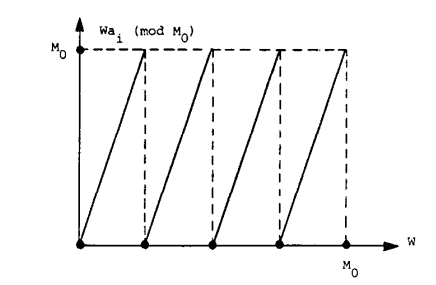
\includegraphics[width=0.6\textwidth, height=0.6\textheight, keepaspectratio]{Dientes_Shamir_1}
        \caption{Gráfica de la función $W \cdot a_{i} \text{ mod } M_{0}$, \cite{artSha}.}
        \label{fig:4.1}
    \end{figure}

    La figura \ref{fig:4.1} representa el gráfico de la función:
    \begin{equation}
        W \cdot a_{i} \text{ mod } M_{0} \text{ , con } 0 \leq W < M_{0}
    \end{equation}
    Esta imagen tiene forma de dientes de sierra. En ella, estamos representando $W$ en el eje horizontal y $M_{0}$ como el valor máximo del eje vertical, ya que es el módulo. La pendiente corresponde con el valor $a_{i}$, al igual que el número de mínimos; y la distancia entre dos mínimos sucesivos es igual a $M_{0}/a_{i}$, que es ligeramente superior a $1$.

    A continuación, vamos a resumir la idea principal para entender cómo se obtienen los valores $M_{0}$ y $W_{0}$. El valor $W_{0}$ verifica que $a'_{1} = W_{0} \cdot a_{1} \text{ mod } M_{0}$, es como máximo de tamaño $2^{dn - n}$. Como la pendiente es $a_{1}$, entonces la distancia horizontal entre $W_{0}$ y el mínimo más cercano de la curva $a_{1}$, no puede ser mayor a $2^{dn - n} / a_{1} \approx 2^{-n}$. Por tanto, la incógnita $W_{0}$ debe estar muy cerca de un mínimo de la curva $a_{1}$. Desafortunadamente, hay demasiados valores de $W_{0}$ y no podemos comprobar todos ellos.

    Sin embargo, podemos aplicar un análisis análogo a la curva $a_{2}$, por lo que $W_{0}$ también debe estar a una distancia de $2^{dn - n + 1} / a_{2} \approx 2^{-n + 1}$ del mínimo de $a_{2}$ más cercano. Consecutivamente, los mínimos de $a_{1}$ y $a_{2}$ deben estar muy cerca entre ellos. Esta condición de proximidad reduce el número de lugares en los que $W_{0}$ puede estar, aunque en la mayoría de casos sigue sin caracterizarlo de forma única.

    De igual manera, si superponemos más de estas funciones sierra en un gráfico, todas las posibles ubicaciones de $W_{0}$ deben estar cerca de un mínimo en cada curva. Así que, en lugar de encontrar un valor específico para $W_{0}$, debemos encontrar los puntos donde estos mínimos se agrupan, denominados \textit{puntos de acumulación}.

    Existe una sencilla regla empírica que podemos usar para tener una idea de cuántas de estas curvas debemos analizar al mismo tiempo, antes de que el conjunto de puntos de acumulación se reduzca a un tamaño manejable. Aunque esta estimación se ha probado en muchos experimentos y parece razonable, no siempre es totalmente precisa.

    Supongamos que $l$ representa la cantidad de curvas en forma de diente de sierra que superponemos en nuestro gráfico. Consideremos el $p$-ésimo mínimo de la curva $a_{1}$, que está situado en $W = pM_{0}/a_{1}$. Así, el mínimo más cercano de la curva $a_{i}$, se encuentra en algún lugar del intervalo:
    \begin{equation}
        [\frac{pM_{0}}{a_{1}} - \frac{M_{0}}{2a_{i}}, \frac{pM_{0}}{a_{1}} + \frac{M_{0}}{2a_{i}}]
    \end{equation}
    cuya longitud es de $\frac{M_{0}}{a_{i}} \approx 1$. A continuación, hacemos una suposición bastante razonable, aunque nada rigurosa, de que la localización real de los distintos mínimos de $a_{i}$ son variables aleatorias que siguen una distribución de probabilidad uniforme. Podemos así, estimar la probabilidad de que los mínimos de las curvas $a_{2}, ... , a_{l}$, estén lo suficientemente cerca del $p$-ésimo mínimo de la curva $a_{1}$, con la siguiente operación:
    \begin{equation}
        2^{-n + 1} \cdot 2^{-n + 2} \cdot \cdot \cdot 2^{-n + l - 1} \approx 2^{-ln + n + l^{2}/2}
    \end{equation}
    Puesto que debemos tener en cuenta también los $a_{1}$ posibles valores de $p$,
    \begin{equation}
        a_{1} \cdot 2^{(-ln + n + l^{2})/2} \approx 2^{dn - ln + n + l^{2}/2}
    \end{equation}
    Este valor es menor que $1$, cuando se verifica la siguiente desigualdad:
    \begin{equation}
        (l - d - 1)n > \frac{l^{2}}{2}
    \end{equation}
    Por último, tomando $n$ suficientemente grande, se verifica:
    \begin{equation}
        l > d + 1
    \end{equation}
    De esta manera, $l$ es una constante que depende de $d$, pero no de $n$. 
    
    La afirmación de que el número esperado de puntos de acumulación es menor que $1$ no es literal, ya que siempre hay al menos un punto de acumulación ``por construcción''. No obstante, es razonable suponer que en situaciones prácticas, cuando $l$ es mayor que $d + 1$, el punto ``construido'' no estará acompañado por otros puntos cercanos cuando se verifique la condición.

    \begin{ejemplo} \cite{artSha}
        Por ejemplo, tomando $n = 100$ y $|M| = 200$, $l = 4$ puede ser un candidato razonable para indicar el número de curvas en forma de diente de sierra.
    \end{ejemplo}

    Sin embargo, todavía tenemos dos problemas: cómo deshacerse de $M_{0}$, cuyo valor aún es desconocido; y cómo encontrar los puntos de acumulación de los mínimos de las $l$ curvas. Un punto a tener en cuenta es que los puntos de acumulación dependen de las pendientes de las curvas, pero no de su tamaño. Por tanto, si dividimos entre $M_{0}$ los dos ejes en la curva $i$-ésima, obtenemos la curva de la siguiente función:
    \begin{equation}
        V \cdot a_{i} \text{ mod } 1 \text{ , con } 0 \leq V < 1
    \end{equation}
    Siendo $V = W/M_{0}$. Además, esta curva es independiente de $M_{0}$, como se aprecia en la imagen:

    \begin{figure}[H]
        \centering
        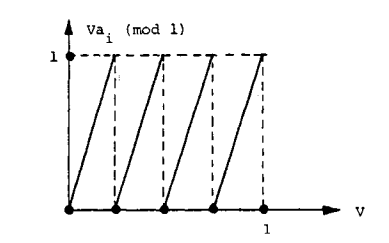
\includegraphics[width=0.6\textwidth, height=0.6\textheight, keepaspectratio]{Dientes_Shamir_2}
        \caption{Gráfica de la función $V \cdot a_{i} \text{ mod } 1$, \cite{artSha}.}
    \end{figure}

    En el nuevo sistemas de coordenadas, la pendiente de la curva sigue siendo $a_{i}$, al igual que el número de mínimos; pero la distancia entre mínimos sucesivos se reduce a $1/a_{i}$. Así, el parámetro $W_{0}$ queda reemplazado por el parámetro $V_{0} = W_{0}/M_{0}$, y la distancia entre este parámetro y el mínimo de la curva $a_{i}$ más cercano, se reduce aproximadamente en $2^{dn}$. El problema de localización de los puntos de acumulación de $l$ mínimos en el nuevo sistema de coordenadas, puede describirse mediante desigualdades lineales con $l$ incógnitas integrales. Las condiciones para que el $p$-ésimo mínimo de $a_{1}$, $q$-ésimo mínimo de $a_{2}$, $r$-ésimo mínimo de $a_{3}$, ..., estén suficientemente próximos entre sí, son las siguientes:
    \begin{align}
        \text{Sean } p,q,r, ... , \text{ enteros, } &&1 \leq p \leq a_{1} - 1 \\
        -\epsilon_{2} \leq \frac{p}{a_{1}}-\frac{q}{a_{2}} \leq \epsilon'_{2} &&1 \leq q \leq a_{2} - 1 \\
        -\epsilon_{3} \leq \frac{p}{a_{1}}-\frac{r}{a_{3}} \leq \epsilon'_{3} &&1 \leq r \leq a_{3} - 1
    \end{align}
    \hspace{5cm}\vdots\hspace{5cm}\vdots
    
    donde $\epsilon_{i}$ y $\epsilon'_{i}$ representan las desviaciones hacia a la derecha y hacia la izquierda de $p/a_{1}$. multiplicando las inecuaciones dobles de la columna izquierda por sus denominadores, obtenemos:
    \begin{align}
        -\delta_{2} \leq pa_{2} &- qa_{1} \leq \delta'_{2} \\
        -\delta_{3} \leq pa_{3} &- ra_{1} \leq \delta'_{3} \\
        &\vdots
    \end{align}
    Aquí se muestra que los valores de $a_{2}, a_{3}, ... ,$ se reducen simultáneamente a valores absolutos pequeños cuando se multiplica por $p$ y se reduce mod $a_{1}$.

    El problema de minimizar simultáneamente dos números mediante multiplicación modulo un tercer número, puede resolverse utilizando un sencillo algoritmo de fracciones continuas. En el caso general, debemos utilizar el algoritmo de programación entera de Lenstra, que aunque es más lento, es polinomial respecto al tamaño de los coeficientes para un número fijo de incógnitas. Este algoritmo es esencialmente un procedimiento de decisión que nos dice si un cierto sistema de desigualdades lineales tiene soluciones enteras. Al utilizar búsqueda binaria en los bits sucesivos de $p$, podemos encontrar todos los puntos de acumulación de las $l$ curvas.

    \begin{figure}[H]
        \centering
        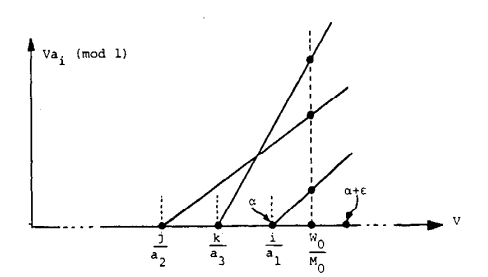
\includegraphics[width=0.6\textwidth, height=0.6\textheight, keepaspectratio]{Dientes_Shamir_3}
        \caption{Sección ampliada del diagrama superpuesto cerca de $V_{0} = \frac{W_{0}}{M_{0}}$, \cite{artSha}.}
    \end{figure}

    Para controlar el tiempo de ejecución del algoritmo y que sea polinomial, debemos añadir un parámetro $k$, el cual se encarga de abortar el programa si se supera cierto número $k$ de puntos de acumulación (tomaremos $k = 100$ por defecto). Un ejemplo extremo de no utilizar este parámetro, sería que todos los $a_{i}$ fueran iguales, por lo que todos los mínimos serían puntos de acumulación. Otra idea que podemos usar es cambiar el valor de $l$ y de $k$, ya que así es posible controlar la fracción de claves para las que el algoritmo no consigue calcular una pareja de valores trampilla.
    
    \begin{observacion}
        Cabe mencionar que no resolver todas las instancias de un problema no es una desventaja grave en el contexto de la criptografía, ya que un criptosistema se vuelve inútil cuando la mayoría de sus claves pueden ser criptoanalizados eficientemente, por lo que no hace falta que se resuelvan todas.
    \end{observacion}

    Podría suceder que un usuario, futuro receptor de un mensaje, permutase los elementos de su clave pública antes de mostrarla. Entonces, $a_{i}$ ya no correspondería al $i$-ésimo elemento más pequeño de la sucesión supercreciente. Aún así, esta variante de Merkle-Hellman puede romperse en tiempo polinómico con esta técnica. Como sólo debemos buscar los $l$ elementos más pequeños, estos se pueden encontrar en $O(n')$ maneras. Dado que $l$ es una constante que no depende de la complejidad de $n$, nuestro método aumenta su complejidad en un factor polinomial. 

    Alternativamente, el criptoanalista puede relajar los valores de $\epsilon$, que representan las desviaciones entre los distintos mínimos de la curva, de modo que el problema de programación entera pueda satisfacerse no sólo cuando se adivinen correctamente los $l$ valores incrementales más pequeños, sino para cualquier elección de $l$ valores lo suficientemente pequeños. Además, si se eligen adecuadamente los nuevos valores de los $\epsilon$, es posible sustituir el factor $O(n')$ por una constante, lo que en aplicaciones prácticas ahorra tiempo.

    El análisis de las primeras $l$ curvas en diente de sierra, nos permite concentrarnos en unas pocas regiones pequeñas en las que debe localizarse el valor real de $V_{0} = W_{0}/M_{0}$. Dentro de estas regiones, las curvas son lineales a trozos con sólo unos pocos puntos de discontinuidad, por lo que sus valores pueden expresarse y compararse sin un análisis excesivo de casos.

    La segunda parte del algoritmo se encarga de descartar en estas regiones, todas aquellas subregiones en las que la sucesión de valores de la curva no sea supercreciente, o su suma sea menor que $1$. Cada punto racional del resto de subregiones corresponde a una pareja de valores trampilla. Además como $V_{0} = W_{0}/M_{0}$ no ha sido descartado, algún subconjunto es no vacío.

    Sea ahora $p$ uno de los valores obtenido por la primera parte del algoritmo. Consideramos el intervalo $[p/a_{1}, (p+1)/a_{1})$ entre $a_{1}$ mínimos sucesivos. El número de puntos de discontinuidad esperados de otras curvas superpuestas en él, es $O(n)$. Sea $V_{1}, ... , V_{s}$ una lista de coordenadas de estos puntos discontinuos ordenadas de manera creciente. Entre cada $V_{t}$ y $V_{t+1}$, todas las curvas $a_{i}$ parecen segmentos lineales simples. El $i$-ésimo segmento lineal puede expresarse así:
    \begin{equation}
        Va_{i} - \tau^{t}_{i} \text{ , con } V_{t} \leq V < V_{t+1}
    \end{equation}
    donde $\tau^{t}_{i}$ es el número de mínimos de $a_{i}$ en $(0, V_{t}]$. Esto es, $\tau^{t}_{i}/a_{i}$ es el punto donde se corta la línea con el eje $V$. A continuación, podemos escribir el rango, tamaño y las condiciones de sucesión supercreciente de la siguiente forma:
    \begin{align}
        &V_{t} \leq V < V_{t+1} \\
        \sum_{i=1}^{n} &(Va_{i} - \tau^{t}_{i}) < 1 \\
        Va_{i} - \tau^{t}_{i} > &\sum_{j=1}^{i-1} (Va_{j} - \tau^{t}_{j}) \text{ , con } i = 2, ... , n
    \end{align}
    La solución de este sistema de inecuaciones lineales en $V$ es un subintervalo de la forma $[V_{t}, V_{t+1})$, posiblemente vacío. Además, se verifica que $W/M$ pertenece a ese subintervalo para algún $p$ y $t$, si y solo si, $M$ y $W$ forman una pareja de valores trampilla.

    Solo falta mencionar que, en caso de que se realice una permutación de elementos de la sucesión supercreciente, es necesario usar también la condición de permutación supercreciente. Como no se puede averiguar la permutación aplicada en tiempo polinomial, debemos usar que toda sucesión supercreciente es una sucesión creciente, para reducir el número de permutaciones posibles a considerar. 

    Para ello, debemos ampliar la definición de la secuencia $V_{1}, ... , V_{s}$, incluyendo no solo los puntos de acumulación, sino también las $V$ coordenadas de las intersecciones entre pares de curvas. Esto puede hacer que aumente el valor de $s$, pasando de $O(n)$ a $O(n^2)$. 
    
    Dentro de cada nuevo rango de valores $[V_{t}, V_{t+1})$, existe una forma clara de ordenar las diferentes curvas verticalmente. Por lo tanto, solo hay una forma posible de organizar sus nombres de manera que la secuencia sea creciente. En particular, de las $n!$ permutaciones posibles, sólo debemos considerar $O(n^2)$ en cada punto de acumulación.
    
    \section{Descripción formal del algoritmo}

    Como ya mencionamos anteriormente, el algoritmo abortará si las $l$ curvas tienen al menos $k$ puntos de acumulación. En esta sección vamos a analizar cómo la fracción de los parámetros $l$ y $k$, influye en la cantidad de fallos del algoritmo y demostraremos que en un modelo probabilístico simplificado, esta fracción pueden hacerse arbitrariamente pequeña.
    
    Por simplificar, asumimos que $a_{1}$ es un valor primo fijo y que $a_{2}, ... , a_{l}$ son variables aleatorias independientes que siguen una distribución de probabilidad uniforme en $[1, a_{1} - 1]$. La condición de que $a_{1}$ sea primo es básicamente para que los inversos modulares estén bien definidos, pero no es esencial y por tanto, se puede reemplazar por otra condición o un análisis más cuidadoso. Por último, asumiremos por simplicidad que las variables del algoritmo de programación entera $\delta_{i}$ y $\delta'_{i}$ coinciden, y denotaremos ambas variables como $\delta$, aunque esto sea un abuso de notación. 

    \begin{definicion} \cite{artSha}
    Para cada $2 \leq i \leq l$, se define $S_{i}$ como el conjunto de indices de mínimos de $a_{1}$ suficientemente cercanos a algún mínimo de $a_{i}$:
        \begin{equation}
            S_{i} = \{1 \leq p \leq a_{1} - 1 \text{ | }\exists \text{ } q_{i} \text{, } 1 \leq q_{i} \leq a_{i} - 1, \text{ tq } -\delta \leq pa_{i} - qa_{1} \leq \delta\}    
        \end{equation}
    \end{definicion}

    Como todos los $S_{i}$ son conjuntos de mínimos de $a_{1}$, su intersección $S_{2} \cap ... \cap S_{l}$, es exactamente el conjunto de puntos de acumulación en los que un mínimo de $a_{1}$, está simultáneamente cerca de los mínimos de todas las demás curvas.

    \begin{lema} \cite{artSha}
        Mostramos ahora una caracterización alternativa al conjunto $S_{i}$ definido previamente, más fácil de manipular:
        \begin{equation}
            S_{i} = \{j_{i}a_{i}^{-1} \text{ mod } a_{1} \text{ | } -\delta \leq j_{i} \leq \delta \text{, } j_{i} \neq 0\}    
        \end{equation}
    \end{lema}

    \begin{proof}
        \begin{equation}
            p \equiv j_{i}a_{i}^{-1} \text{ mod } a_{1}
        \end{equation}
        equivale a
        \begin{equation}
            pa_{i} \equiv j_{i}a_{i}^{-1}a_{i} \text{ mod } a_{1} \equiv j_{i} \text{ mod } a_{1}
        \end{equation}
        y por tanto, existe $q_{i}$ tal que:
        \begin{equation}
            pa_{i} = j_{i} + q_{i}a_{1}
        \end{equation}
        Como $-\delta \leq j_{i} \leq \delta$, $pa_{i}-q_{i}a_{1}$ cumple las condiciones. Finalmente, el valor $j_{i} = 0$ no está permitido en la definición de $S_{i}$, por lo que se restringe ese valor.
    \end{proof}

    La equivalencia $p \equiv j_{i}a_{i}^{-1} \text{ mod } a_{1}$, establece para cada $p$, una relación uno a uno entre la secuencia $a_{2}, ... , a_{l}$ y la secuencia $j_{2}, ... , j_{l}$. El valor $p$ es un punto de acumulación de $a_{2}, ... , a_{l}$, sí y solo si todos los correspondientes $j_{i}$ son enteros no nulos pertenecientes a $[-\delta, \delta]$. De manera alternativa, cuando $p$ y una secuencia de $j_{i}$ son dados, existe una única secuencia de $a_{i}$ para la cual $p$ es un punto de acumulación con estos $j_{i}$ índices.

    \begin{lema} \cite{artSha} \label{lem:4.5}
        Sean $p'$ y $p''$ dos puntos de acumulación de $a_{2}, ... , a_{l}$, y sean $j'_{2}, ... , j'_{l}$ y $j''_{2}, ... , j''_{l}$ las secuencias de sus índices $j$ asociados. Si $\delta < \sqrt{a_{1}/2}$, entonces ambas secuencias son múltiplos de una secuencia común $j_{2}, ... , j_{l}$ donde se verifica que gcd($j_{2}, ... , j_{l}$) = $1$.
    \end{lema}

    \begin{proof}
        Partiendo de $p' \equiv j'_{i}a_{i}^{-1} \text{ mod } a_{1}$, y $p'' \equiv j''_{i}a_{i}^{-1} \text{ mod } a_{1}$, podemos obtener:
        \begin{equation}
            a_{i} \equiv j'_{i}p'^{-1} \equiv j''_{i}p''^{-1} \text{ mod } a_{1}
        \end{equation}
        que, tras simplificación:
        \begin{equation}
            j'_{i}j_{i}^{''-1} \equiv p'p^{''-1} \text{ mod } a_{1}
        \end{equation}
        Como la parte derecha de la equivalencia no depende de $i$, para cualquier $s$ y $t$ se verifica:
        \begin{align}
            j'_{s}j_{s}^{''-1} &\equiv j'_{t}j_{t}^{''-1} \text{ mod } a_{1} \\
            j'_{s}j''_{t} &\equiv j'_{t}j''_{s} \text{ mod } a_{1}
        \end{align}
        Por la suposición de $\delta$, cada producto $j'j"$ sólo puede estar en $[\frac{-a_{1}}{2}, \frac{a_{1}}{2}]$, por lo que se cumple (incluso sin módulo):
        \begin{equation}
            j'_{s}j''_{t} = j'_{t}j''_{s}
        \end{equation}
        Esta igualdad se verifica para todo $s$ y $t$ sólo si las secuencias $j'$ y $j"$ son múltiplos racionales entre sí. Como contienen sólo números enteros, deben ser múltiplos de alguna secuencia común $j_{2}, ... , j_{l}$ de enteros, cuyo gcd sea $1$.
    \end{proof}

    \begin{corolario}
        Cuando $\delta < \sqrt{a_{1}/2}$ y la intersección $S_{2} \cap ... \cap S_{l}$ es no vacía, hay un punto de acumulación cuya secuencia de índices es $j_{2}, ... , j_{l}$ y su gcd es $1$, y además todos los puntos de acumulación restantes se obtienen multiplicando la secuencia de $j_{i}$ por $1, -1, 2, -2, 3, -3, ...$ etc. hasta que un elemento supere el valor de $\delta$.

        Cuando $\delta \geq \sqrt{a_{1}/2}$, la intersección $S_{2} \cap ... \cap S_{l}$ es más complicada de analizar y no tenemos ninguna caracterización sencilla.
    \end{corolario}

    \begin{definicion} \cite{artSha}
        Denotaremos como $N(l, k, \delta)$ al número de secuencias $a_{2}, ... , a_{l}$ en $[1, a_{1} - 1]$, para las que la intersección $S_{2} \cap ... \cap S_{l}$ contiene al menos $k$ puntos cuando la distancia tolerable es $\delta$.
    \end{definicion}

    Nos interesa la probabilidad condicional de que las $l$ curvas tengan al menos $k$ puntos de acumulación, cuando se sabe que tienen al menos uno. Dado que lo primero implica lo segundo, esta probabilidad condicional es simplemente:
    \begin{equation}
        \frac{N(l, k, \delta)}{N(l, 1, \delta)} 
    \end{equation}

    \begin{lema} \cite{artSha}
        Para cada $\delta < \sqrt{a_{1}/2}$ y $l \geq 3$, hay una constante $\tau$ en $[3/\pi^{2}, 1/2]$ que depende solo de $l$, tal que:
        \begin{equation}
            N(l, 1, \delta) \approx \tau(a_{1} - 1)(2\delta)^{l - 1}
        \end{equation}
    \end{lema}
    
    \begin{proof}
        Podemos calcular el número de secuencias $a_{2}, ... , a_{l}$ que tienen al menos un punto de acumulación, contando el número de secuencias $p, a_{2}, ... , a_{l}$, donde $p$ es un punto de acumulación de $a_{i}$. Este número es igual al número de secuencias $p, j_{2}, ... , j_{l}$, donde $p$ es arbitrario y los $j_{i}$ son enteros no nulos pertenecientes a $[-\delta, \delta]$, equivalentamente, $(a_{1} - 1)(2\delta)^{l - 1}$. Para corregir el cálculo, tomamos solamente secuencias de $j_{i}$ cuyo gcd sea $1$. Por el lema \ref{lem:4.5}, para cada $a_{i}$, hay exactamente dos secuencias $j_{i}$ con puntos de acumulación y con gcd = $1$ (cada secuencia es la negación de la otra). 
        
        Para $l = 3$, la fracción de secuencias enteras de longitud $l - 1$ cuyo gcd = $1$, converge a $6/\pi^{2}$ y para valores superiores de $l$ esta fracción se aproxima a $1$. Dado que cada secuencia $a_{i}$ con puntos de acumulación se cuenta exactamente dos veces, tenemos que dividir esta constante por $2$ para obtener la constante correcta $\tau$.
    \end{proof}

    \begin{lema} \cite{artSha}
        Si $\delta < \sqrt{a_{1}/2}$, entonces $N(l, k, \delta) \leq N(l, 1, \frac{\delta}{k/2})$.
    \end{lema}
    
    \begin{proof}
        Sea $j_{2}, ... , j_{l}$ la secuencia de índices con gcd = $1$, cuya existencia está garantizada por el lema \ref{lem:4.5}. Como $a_{2}, ... , a_{l}$ tiene al menos $k$ puntos de acumulación, esta secuencia de $j_{i}$ puede ser multiplicada por $k/2$ y todos sus elementos seguirán perteneciendo a $[-\delta, \delta]$. Como consecuencia, todos los $j_{i}$ originales están en $[\frac{-\delta}{k/2}, \frac{\delta}{k/2}]$, y por tanto, la sucesión $a_{i}$ tiene al menos un punto de acumulación incluso cuando el límite $\delta$ se sustituye por otro límite más estricto $\frac{\delta}{k/2}$.
    \end{proof}

    Llegamos a continuación al teorema principal de este capítulo.

    \begin{teorema} \cite{artSha} \label{theo:4.10}
        Cuando $\delta < \sqrt{a_{1}/2}$ y $l \geq 3$, el valor de la probabilidad condicionada $\frac{N(l, k, \delta)}{N(l, 1, \delta)}$ es como máximo $(\frac{1}{k/2})^{l - 1}$. 
    \end{teorema}

    \begin{proof}
        \begin{align}
           \frac{N(l, k, \delta)}{N(l, 1, \delta)} &\leq \frac{N(l, 1, \delta/(k/2))}{N(l, 1, \delta)} \\
            &= \frac{\tau(a_{1} - 1)(2\delta/(k/2))^{l - 1}}{\tau(a_{1} - 1)(2\delta)^{l - 1}} \\
            &= (\frac{1}{k/2})^{l - 1}
        \end{align}
    \end{proof}

    \begin{ejemplo} \cite{artSha}
        Tomando $l = 4$, $k = 100$ y $\delta < \sqrt{a_{1}/2}$, la probabilidad de que $4$ curvas de dientes en sierra tengan al menos $100$ puntos de acumulación cuando se sabe que tienen al menos uno, es de $(1/50)^{3} = 1/125000$. Por tanto, si utilizamos el algoritmo de Lenstra (algoritmo L$^{3}$) para encontrar los puntos de acumulación y se aborta tras encontrar $100$ puntos, la probabilidad de fallo es insignificante.
    \end{ejemplo}

    En nuestro análisis aplicado, $\delta$ es aproximadamente $2^{dn - n}$ y $a_{1}$ es aproximadamente $2^{dn}$. Así, la condición $\delta < \sqrt{a_{1}/2}$ es equivalente a la condición $d < 2$. Shamir no pudo probar el limite superior del Teorema \ref{theo:4.10} para criptosistemas en los que la relación $d$, del tamaño del módulo entre el número de elementos, es mayor que $2$. Sin embargo, Jeff Lagarias anunció posteriormente un límite superior diferente aplicable a todo el rango $1 < d < \infty$.

    \section{Análisis del algoritmo}

    En el apartado anterior se ha mostrado que todos los criptosistemas de una iteración de Merkle-Hellman pueden ser rotos en tiempo polinomial con probabilidad de fallo arbitrariamente pequeña. La parte que más tiempo necesita es la aplicación del algoritmo de programación entera de Lenstra, ya que en el peor caso su complejidad es polinomial en $n$, pero exponencial en $l$.

    Una característica muy importante del ataque propuesto, es que se dirige a la clave pública y no a los textos cifrados individuales. De este modo, el criptoanalista puede abordar claves de reserva o de bajo volumen, incluso antes de que se utilicen por primera vez. Además, podría dedicar meses de tiempo computacional a cada clave, con el fin de facilitar posteriormente la decodificación del mensaje en microsegundos.

    El problema más importante que queda abierto en este capítulo, es la seguridad criptográfica sobre los criptosistemas de Merkle-Hellman de varias iteraciones. En cada iteración, el módulo elegido aleatoriamente debe ser mayor que la suma de los elementos, por lo que las multiplicaciones modulares inversas reducen simultáneamente el tamaño de los elementos al menos en $log(n)$. En principio, esta condición permite hallar el único intervalo en el que se encuentra $W/M$, pero no $W$ ni $M$. 

    En el caso de la mochila de iteración simple, cualquier pareja trampilla era útil, ya que generaba una secuencia supercreciente fácilmente resoluble. En el caso de las mochilas de iteración múltiple, sólo los valores $W$ y $M$ correctos permiten al criptoanalista hacer la multiplicación inversa correctamente y atacar las iteraciones internas una a una.

\endinput
\chapter{Ataques por baja densidad} \label{ch:quinto-capitulo}

     El objetivo de este capítulo consiste en abordar otros ataques a criptosistemas distintos al que se examinó en el capítulo \ref{ch:cuarto-capitulo}. En esta sección, nos enfocaremos en la vulnerabilidad de criptosistemas de baja densidad, como Merkle-Hellman iterado, cuya ruptura no fue tratada en el capítulo anterior. Las principales referencias bibliográficas de este capítulo son: \cite{artLagOdl}, \cite{artLLL}, \cite{artCoster} y \cite{tfgLag}.
    
    \section{Algoritmo L\texorpdfstring{$^3$}{3}}

    Durante el transcurso de este capítulo, exploraremos diversos ataques criptográficos caracterizados por su preferencia a operar con criptosistemas de poca densidad. Ambos utilizan el algoritmo L$^{3}$, por lo que iniciaremos el capítulo proporcionando una explicación detallada de dicho algoritmo, para posteriormente adentrarnos en el análisis de cada uno de estos ataques.

    El algoritmo L$^{3}$ o LLL, toma su nombre de sus diseñadores A. K. Lenstra, H. W. Lenstra, Jr. y L. Lovász. Es un algoritmo de simplificación de retículos publicado en $1982$, que parte de una base con coordenadas n-dimensionales de un retículo y devuelve una base reducida del mismo retículo, en tiempo polinomial.

    Aunque nos adentraremos en cada uno de los pasos de este algoritmo, primeramente debemos definir ciertos conceptos que nos serán necesarios.

    \begin{definicion} \cite{artLagOdl}
        Sea el vector $v = (v_{1}, ... , v_{n}) \in \mathbb{R}^{n}$, definimos su \textit{norma euclídea} o \textit{longitud}, de la siguiente forma:
        \begin{equation}
            \|v\|^{2} = \sum_{i=1}^{n} v_{i}^{2}
        \end{equation}
    \end{definicion}
    
    Llamaremos \textit{vector corto} a un vector cuya longitud sea ``pequeña''. Buscamos encontrar el vector más corto, es decir, dada una base $B$ hallar el $v \in \mathbb{B}$ tal que $\| v \| \leq \| x \| \text{, } \forall x\in B$.  

    \begin{definicion} \cite{artLagOdl}
        Un \textit{retículo de enteros} $L$ es un subgrupo aditivo de $\mathbb{Z}^{n}$, que contiene $n$ vectores linealmente independientes sobre $\mathbb{R}^{n}$.
    \end{definicion}

    \begin{definicion} \cite{artLagOdl}
        Una \textit{base} $(v_{1}, ... , v_{n})$ de un retículo de enteros $L$ es un conjunto de elementos de $L$ que verifica:
        \begin{equation}
            L = \sum_{i=1}^{n} \mathbb{Z}v_{i} = \mathbb{Z}v_{1} \oplus \cdot \cdot \cdot \oplus \mathbb{Z}v_{n}
        \end{equation}
    \end{definicion}

    Representamos una base del retículo $L$ mediante la matriz de base $n$ x $n$:
    \begin{equation}
        V = 
        \begin{bmatrix}
            v_{1}  \\
            \vdots \\
            v_{n}  \\
        \end{bmatrix}
    \end{equation}
    formada por los vectores de la base puestos por filas. Además, se verifica que si $V_{1}$ y $V_{2}$ son dos matrices de bases del mismo retículo $L$, existe una matriz unimodular $U \in GL(n, \mathbb{Z})$, que verifica que:
    \begin{equation}
        U \cdot V_{1} = V_{2}
    \end{equation}
    De igual forma, si $V$ es una matriz de base del retículo $L$, y $U \in GL(n, \mathbb{Z})$, entonces $U \cdot V$ es una matriz de base de $L$.

    \begin{definicion} \cite{artLLL}
        El \textit{determinane} $d(L)$ de un retículo $L \subset \mathbb{R}^{n}$ se define por:
        \begin{equation}
            det(L) = \left| det(v_{1}, ... , v_{n}) \right|
        \end{equation}
        donde los elementos $v_{i}$ son los vectores de una base puestos por columnas. Este valor positivo no depende de la base escogida.
    \end{definicion}

    Ahora, sea $(v_{1}, ... , v_{n})$ una base del retículo $L \subset \mathbb{R}^{n}$, y sea $(v'_{1}, ... , v'_{n})$ su ortogonalización de Gram-Schmidt. Denotamos como $(\mu_{ij})$ a los elementos de la matriz $M$ de Gram-Schmidt que verifica $V = M \cdot V'$, donde $V$ es la matriz con vector $v_{i}$ en la fila $i$-ésima (respectivamente con $V'$).
    
    \begin{definicion} \cite{artLagOdl} \label{def:5.5}
        Una base de un retículo $(v_{1}, ... , v_{n})$ diremos que es \textit{$\alpha$-reducida} o \textit{LLL-reducida con parámetro $\alpha$}, si satisface ambas propiedades:
        \begin{enumerate}
            \item $\left| \mu_{ij} \right| \leq \frac{1}{2}$, para $1 \leq j < i \leq n$
            \item $\| v'_{i} + \mu_{i,i-1} v'_{i-1} \|^{2} \geq \alpha\| v'_{i-1} \|^{2}$, para $2 \leq i \leq n$ 
        \end{enumerate}
        Esta última condición se conoce como \textit{condición de intercambio}.
    \end{definicion}

    La idea intuitiva de la primera condición, nos dice que cada vector $v_{i}$ de la base es ``casi ortogonal'' al generador de los vectores anteriores, ya que por Gram-Smith:
    \begin{equation}
        \langle v_{1}, ... , v_{i-1} \rangle = \langle v'_{1}, ... , v'_{i-1} \rangle
    \end{equation}
    Por otro lado, la segunda condición nos indica que al intercambiar $v_{i-1}$ y $v_{i}$, y aplicar de nuevo el método de ortogonalización de Gram-Schmidt, se puede generar un vector ``un poco más corto''. 

    Teniendo en cuenta que $\frac{1}{4} < \alpha < 1$, tomaremos el valor estándar del parámetro como $\alpha = \frac{3}{4}$. Nuestro objetivo es demostrar que para cualquier retículo $L \subset \mathbb{R}^{n}$ y cualquier base $\alpha$-reducida de $L$, el algoritmo L$^{3}$ genera una base $\alpha$-reducida de $L$ en un número de pasos acotados por un polinomio dependiente de $n$.

    \begin{definicion} \cite{tfgLag}
        Definimos el parámetro secundario $\beta$ como:
        \begin{equation}
            \beta = \frac{4}{4\alpha - 1} \text{ , con } \frac{1}{4} < \alpha < 1
        \end{equation}
        Las dos condiciones de $\alpha$ son para que se verifique $\beta > \frac{4}{3}$. Asimismo, para el valor estándar $\alpha = \frac{3}{4}$, se obtiene $\beta = 2$. 
    \end{definicion}
    
    \begin{proposicion} \cite{artLLL}
        Sea $(v_{1}, ... , v_{n})$ una base $\alpha$-reducida de un retículo $L \subset \mathbb{R}^{n}$, y sea $(v'_{1}, ... , v'_{n})$ su ortogonalización de Gram-Schmidt. Entonces:
        \begin{enumerate}
            \item $\left| v_{j} \right|^{2} \leq \beta^{i-j} \left| v'_{i} \right|^{2}$, para $1 \leq j \leq i \leq n$
            \item $det(L) \leq \left| v_{1} \right| \left| v_{2} \right| \hdots \left| v_{n} \right| \leq \beta^{n(n-1)/4} \cdot det(L)$
            \item $\left| v_{1} \right| \leq \beta^{(n-1)/4} \cdot det(L)^{1/n}$
        \end{enumerate}
        donde $\beta$ es el parámetro definido previamente.
    \end{proposicion}

    \begin{proof}
        Partiendo de la definición \ref{def:5.5}, podemos ver que:
        \begin{equation}
            \left| v'_{i} \right|^{2} \geq (\alpha - \mu_{i,i-1}^{2}) \left| v'_{i-1} \right|^{2} \geq (\alpha - \frac{1}{4})\left| v'_{i-1} \right|^{2} = \frac{1}{\beta} \left| v'_{i-1} \right|^{2}
        \end{equation}
        Por tanto, $\left| v'_{i-1} \right|^{2} \leq \beta \left| v'_{i} \right|^{2}$, y por inducción obtenemos:
        \begin{equation} \label{eq:5.1}
            \left| \smash[b]{v'_{j}} \right|^{2} \leq \beta^{i-j} \left| v'_{i} \right|^{2} \text{, para } 1 \leq j \leq i \leq n
        \end{equation}
        La definición de $v'_{i}$ en la ortogonalización de Gram-Schmidt se puede reescribir como $v_{i} = v'_{i} + \sum_{j=1}^{i-1} \mu_{ij}v'_{j}$. Asimismo, como $v'_{1}, ... , v'_{n}$ son ortogonales, $v_{i}^{2} = v_{i}^{'2} + \sum_{j=1}^{i-1} \mu_{ij}^{2} \left| \smash[b]{v'_{j}} \right|^{2}$. Con esto y a partir de la definición \ref{def:5.5}, llegamos a:
        \begin{equation}
            \left| v_{i} \right|^{2} = \left| v'_{i} \right|^{2} + \sum_{j=1}^{i-1} \frac{1}{4}\beta^{i-j} \left| v'_{i} \right|^{2} = (1 + \frac{1}{4} \sum_{j=1}^{i-1} \beta^{i-j}) \left| v'_{i} \right|^{2}
        \end{equation}
        Aplicando la fórmula de la suma de una progresión geométrica, obtenemos:
        \begin{equation}
            \left| v_{i} \right|^{2} \leq (1 + \frac{1}{4} \cdot \frac{\beta^{i} - \beta}{\beta - 1}) \left| v'_{i} \right|^{2}
        \end{equation}
        Ahora, vamos a aplicar inducción sobre $i$ para demostrar lo siguiente:
        \begin{equation}
            1 + \frac{1}{4} \cdot \frac{\beta^{i} - \beta}{\beta - 1} \leq \beta^{i-1}
        \end{equation}
        Para el primer caso, tomando $i=1$ es trivial. Para el paso de inducción es suficiente probar que:
        \begin{equation}
            1 + \frac{1}{4} \cdot \frac{\beta^{i+1} - \beta}{\beta - 1} \leq \beta (1 + \frac{\beta^{i} - \beta}{4(\beta - 1)})
        \end{equation}
        Como $\beta > \frac{4}{3}$, podemos multiplicar por $4(\beta-1)$ y simplificar, obteniendo:
        \begin{equation}
            3\beta^{2} - 7\beta + 4 = (\beta -1)(3\beta-4) \geq 0
        \end{equation}
        Por tanto, ahora tenemos:
        \begin{equation} \label{eq:5.2}
            \left| v_{i} \right|^{2} \leq \beta^{i-1} \left| v'_{i} \right|^{2}
        \end{equation}
        Usando la fórmula \eqref{eq:5.1}:
        \begin{equation}
            \left| v_{j} \right|^{2} \leq \beta^{j-1} \left| \smash[b]{v'_{j}} \right|^{2} \leq \beta^{i-1} \left| v'_{i} \right|^{2} \text{, para } 1 \leq j \leq i \leq n
        \end{equation}
        Por lo que queda demostrado el apartado $(1)$. Por el teorema de Gram-Schmidt, sabemos que:
        \begin{equation}
            det(L) = \left| v'_{1} \right| \left| v'_{2} \right| \hdots \left| v'_{n} \right| \leq \left| v_{1} \right| \left| v_{2} \right| \hdots \left| v_{n} \right|
        \end{equation}
        A partir de la ecuación \eqref{eq:5.2},
        \begin{equation}
            \left| v_{1} \right|^{2} \left| v_{2} \right|^{2} \hdots \left| v_{n} \right|^{2} \leq \beta^{0 + 1 + \hdots + (n-1)} \left| v'_{1} \right|^{2} \left| v'_{2} \right|^{2} \hdots \left| v'_{n} \right|^{2}
        \end{equation}
        y por tanto,
        \begin{equation}
            \left| v_{1} \right| \left| v_{2} \right| \hdots \left| v_{n} \right| \leq \beta^{n(n-1)/4} \left| v'_{1} \right| \left| v'_{2} \right| \hdots \left| v'_{n} \right| = \beta^{n(n-1)/4} \cdot det(L)
        \end{equation}
        Por lo que queda demostrado el apartado $(2)$. Por último, fijando $j = 1$ en el apartado $(1)$, se tiene:
        \begin{equation}
            \left| v_{1} \right|^{2} \leq \beta^{i-1} \left| v'_{i} \right|^{2} \text{, con } 1 \leq i \leq n
        \end{equation}
        Tomando el producto $i = 1, ... , n$:
        \begin{equation}
            \left| v_{1} \right|^{2n} \leq \beta^{0 + 1 + \hdots + (n-1)} \left| v'_{1} \right|^{2} \left| v'_{2} \right|^{2} \hdots \left| v'_{n} \right|^{2} = \beta^{n(n-1)/2} \cdot det(L)^{2}
        \end{equation}
        Finalmente, tras tomar la raiz de $2n$, queda demostrado el apartado $(3)$.
    \end{proof}

    \begin{teorema} \cite{artLLL}
        Sea $(v_{1}, ... , v_{n})$ una base $\alpha$-reducida del retículo $L \subset \mathbb{R}^{n}$, e $y \in L$ un vector no nulo del retículo, entonces:
        \begin{equation}
            \left| v_{1} \right|^{2} \leq \beta^{n-1} \left| y \right|^{2}
        \end{equation}
    \end{teorema}

    \begin{proof}
        Sea $(v'_{1}, ... , v'_{n})$ la ortogonalización de Gram-Schmidt de $(v_{1}, ... , v_{n})$. Por la definición de base $\alpha$-reducida, para $2 \leq i \leq n$, tenemos:
        \begin{equation}
            \left| v'_{i} \right|^{2} \geq (\alpha - \mu_{i,i-1}^{2}) \left| v'_{i-1} \right|^{2} \geq (\alpha - \frac{1}{4})\left| v'_{i-1} \right|^{2} = \frac{1}{\beta} \left| v'_{i-1} \right|^{2}
        \end{equation}
        Como $v_{1} = v'_{1}$, 
        \begin{equation}
            \left| v_{1} \right|^{2} = \left| v'_{1} \right|^{2} \leq \beta \left| v'_{2} \right|^{2} \leq \beta^{2} \left| v'_{3} \right|^{2} \leq \cdot \cdot \cdot \leq \beta^{n-1} \left| v'_{n} \right|^{2} 
        \end{equation}
        por lo que tenemos:
        \begin{equation}
            \left| v'_{i} \right|^{2} \geq \beta^{-(i-1)} \left| v_{1} \right|^{2} \text{, para } 1 \leq i \leq n
        \end{equation}
        Como consecuencia de Gram-Schmidt, se sabe que para cualquier $y \in L$ no nulo:
        \begin{equation}
            \left| y \right| \geq min\{\left| v'_{1} \right|, ... , \left| v'_{n} \right|\}
        \end{equation}
        por tanto,
        \begin{equation}
            \left| y \right|^{2} \geq min\{\left| v'_{1} \right|^{2}, ... , \left| v'_{n} \right|^{2}\} \geq \beta^{-(n-1)} \left| v_{1} \right|^{2}
        \end{equation}
        Finalmente, despejando llegamos al resultado deseado:
        \begin{equation}
            \left| v_{1} \right|^{2} \leq \beta^{n-1} \left| y \right|^{2}
        \end{equation}
    \end{proof}

    Cabe destacar que el resultado anterior es el caso un particular, con $m = 1$, del siguiente resultado más general, cuya demostración obviaremos.

    \begin{teorema} \cite{artLLL}
        Sea $(v_{1}, ... , v_{n})$ una base $\alpha$-reducida del retículo $L \subset \mathbb{R}^{n}$, e $(y_{1}, ... , y_{m}) \in L$, $m$ vectores linealmente independientes del retículo, entonces, para $1 \leq j \leq m$ se verifica:
        \begin{equation}
            \left| v_{j} \right|^{2} \leq \beta^{n-1} max\{\left| y_{1} \right|^{2}, ... , \left| y_{m} \right|^{2}\}
        \end{equation}
    \end{teorema}

    Tras todo lo explicado, llegamos al objetivo principal de este primer apartado: el Algoritmo L$^{3}$. Para ello, incluimos el código \cite{tfgLag} tanto del algoritmo principal, como de dos funciones utilizadas en él:
    
    \begin{algorithm}[H]
        \caption{Función reduce($k, l$)}
        \textbf{Input:} Índices de los valores que se van a ``ortogonalizar''. \\
        \textbf{Output:} Base y coeficientes de la ortogonalización de Gram-Schmidt tras la modificación.
        \bigskip
        \begin{algorithmic}[1]
            \If{$\left| \mu_{kl} \right| > 1/2$}
            \State $y_{k} = y_{k} - [\mu_{kl}] y_{l}$
            \For{$j$ from $1$ to $l-1$}
            \State $\mu_{kj} = \mu_{kj} - [\mu_{kl}] \mu_{lj}$
            \EndFor
            \State $\mu_{kl} = \mu_{kl} - [\mu_{kl}]$
            \EndIf
        \end{algorithmic}
    \end{algorithm}

    Esta primera función, hace que $y_{k}$ sea ``casi ortogonal'' a $y_{l}$. Como $[\mu_{kl}]$ es el entero más cercano al coeficiente de Gram-Schmidt, es la mejor reducción posible. Después, actualiza la base y los coeficientes de la ortogonalización de Gram-Schmidt.
    
    \begin{algorithm}[H]
        \caption{Función exchange($k$)}
        \textbf{Input:} Índice del valor que se va a intercambiar con su anterior. \\
        \textbf{Output:} Base y coeficientes de la ortogonalización de Gram-Schmidt tras el intercambio. 
        \bigskip
        \begin{algorithmic}[1]
            \State $z = y_{k-1}$; $y_{k-1} = y_{k}$; $y_{k} = z$
            \State $v = \mu_{k, k+1}$; $\delta = \gamma'_{k} + v^{2} \cdot \gamma'_{k-1}$ 
            \State $\mu_{k, k-1} = v \cdot \gamma'_{k-1} / \delta$; $\gamma'_{k} = \gamma'_{k}\gamma'_{k-1}/\delta$; $\gamma'_{k-1} = \delta$
            \For{$j$ from $1$ to $k-2$}
            \State $t = \mu_{k-1, j}$; $\mu_{k-1, j} = \mu_{kj}$; $\mu_{kj} = t$
            \EndFor
            \For{$i$ from $k+1$ to $n$}
            \State $\psi = \mu_{ik}$; $\mu_{ik} = \mu_{i, k-1} - v \cdot \mu_{ik}$; $\mu_{i,k-1} = \mu_{k, k-1}\mu_{ik} + \psi$
            \EndFor
        \end{algorithmic}
    \end{algorithm}

    Esta otra función, intercambia los vectores $y_{k-1}$ e $y_{k}$. Luego, actualiza la base y los coeficientes de la ortogonalización de Gram-Schmidt, y los devuelve.

    \begin{algorithm}[H]
        \caption{Algoritmo L$^{3}$}
        \textbf{Input:} Una base $(x_{1}, ... , x_{n})$ del retículo $L \subset \mathbb{R}^{n}$ y el parámetro $\alpha \in \mathbb{R}$ verificando $\frac{1}{4} < \alpha < 1$. \\
        \textbf{Output:} Una base $\alpha$-reducida $(y_{1}, ... , y_{n})$ del retículo $L \subset \mathbb{R}^{n}$.
        \bigskip
        \begin{algorithmic}[1]
            \For{$i$ from $1$ to $n$}
            \State $y_{i} = x_{i}$
            \EndFor
            \For{$i$ from $1$ to $n$}
            \State $y'_{i} = y_{i}$
            \For{$j$ from $1$ to $i-1$}
            \State $\mu_{ij} = (y_{i} \cdot y'_{j}) / \gamma'_{j}$ 
            \State $y'_{i} = y'_{i} - \mu_{ij} \cdot y'_{j}$
            \EndFor
            \State $\gamma'_{i} = y'_{i} \cdot y'_{i}$
            \EndFor
            \State $k = 2$
            \While{$k \leq n$}
            \State \textbf{reduce}($k, k-1$)
            \If{$\gamma'_{k} \geq (\alpha - \mu_{k, k-1}^{2}) \gamma'_{k-1}$}
            \For{$l$ from $k-2$ to $1$}
            \State \textbf{reduce}($k, l$)
            \EndFor
            \State $k = k+1$
            \Else
            \State \textbf{exchange}($k$)
            \If{$k > 2$}
            \State $k = k-1$
            \EndIf
            \EndIf
            \EndWhile
        \end{algorithmic}
    \end{algorithm}

    Por último, el algoritmo LLL realiza una copia de los vectores de entrada, aplica el proceso de ortogonalización de Gram-Schmidt y finalmente llama a las dos funciones previas para que reduzcan e intercambien los vectores obtenidos. Estos vectores se modifican continuamente a lo largo del algoritmo, de tal manera que siempre forman parte de una base del retículo $L$.

    \newpage

    \section{Ataque de Lagarias-Odlyzko}

    En esta sección se presenta el algoritmo diseñado por J. C. Lagarias y A. M. Odlyzko \cite{artLagOdl}, para resolver instancias del problema de la mochila. Su método implica transformar la instancia original del problema y luego aplicar el algoritmo de reducción de bases de retículos, para así determinar la solución. El rendimiento del algoritmo propuesto se analiza detenidamente, y aunque este algoritmo siempre se detiene en tiempo polinómico, no siempre encuentra una solución cuando existe.

    Para caracterizar el algoritmo, usaremos el concepto de densidad, visto en la definición \ref{def:3.8}, donde $n$ representa la cantidad de elementos del conjunto. Así, para ``casi todos'' los casos con densidad $d < 0.645$, el vector que estamos tratando de encontrar resulta ser el vector más corto no nulo del retículo. Asimismo, tras realizar exhaustivas pruebas computacionales, se observa que este algoritmo es efectivo para densidades $d < d_{c}(n)$, donde $d_{c}(n)$ es un umbral. Como consecuencia, este enfoque proporciona una solución de tiempo polinómico a los sistemas de cifrado del problema de la mochila, lo que implica que puede comprometerlos si la velocidad de transmisión de información es menor que de $d_{c}(n)$, cuando $n \rightarrow \infty$.

    \subsection{Preludio al método}

    Tras la publicación del criptoanálisis de Shamir en $1983$, que como ya sabemos, anunciaba un método para romper el criptosistema de clave pública más simple de Merkle-Hellman, se propusieron otros ataques para criptosistemas más complicados. Esos ataques estaban todos basados en la idea de recuperar la información trampilla oculta en los valores de los pesos. Sin embargo, aquí se propone un método denominado ``Algorithm SV'' (Short Vector), que localiza la solución del problema de la mochila directamente, sin intentar buscar la información trampilla.

    Este nuevo método consiste en transformar el problema inicial, en el problema de encontrar el vector más corto $e$ en un retículo de enteros $L$. Tras esto, se aplica el algoritmo previo de reducción de bases de retículos para obtener una base reducida. El método se considera exitoso cuando el vector $e$ se encuentra en la base reducida, y en tal caso, podemos derivar una solución a partir del vector obtenido.

    Recordemos que al explicar el problema de la mochila por primera vez, definíamos $a = \{a_{1}, ... , a_{n}\} \subseteq \mathbb{N}^{*}$ como el conjunto de pesos del problema, y $S \in \mathbb{N}^{*}$ la capacidad total de la mochila. Este recordatorio de la notación es importante para lo que explicaremos a continuación.

    El principal resultado de esta sección se centra en el análisis del rendimiento del Algoritmo SV, dado que se muestra exitoso en la resolución de problemas de suma de subconjuntos de baja densidad de la siguiente forma:

    \newpage
    
    \begin{enumerate}
        \item Para ``casi todos'' los problemas de la mochila cuya $d(a) < 0.645$, el vector $e$ es el vector no nulo más corto del retículo $L$.
        \item  Para ``casi todos'' los problemas de la mochila resolubles con $n$ pesos que tienen $d(a) < (2 - \epsilon)(log_{2} (\frac{4}{3}))^{-1}n^{-1}$, para cualquier $\epsilon > 0$ fijo, el algoritmo encuentra una solución.
    \end{enumerate}
    
    Lagarias y Odlyzko explican en su artículo que el primer resultado es el más exacto posible, en el sentido de que ya no se cumple si se reemplaza por $0.646$, según las heurísticas utilizadas. Por otro lado, el segundo resultado es más débil de lo que parece a simple vista, ya que no se garantiza que el algoritmo L$^{3}$ produzca el vector más corto no nulo $v_{min}$ del retículo $L \subset \mathbb{Z}^{n}$, simplemente produce uno de ellos. 

    El método que presentamos utiliza el algoritmo L$^{3}$, ya que es el algoritmo original del artículo \cite{artLagOdl}. Además, funciona de manera satisfactoria para encontrar vectores razonablemente cortos de un retículo en tiempo de ejecución polinómico. Sin embargo, en lugar de usar el Algoritmo SV, se podrían realizar modificaciones sustituyendo el algoritmo L$^{3}$ por otro que encuentre vectores cortos de un retículo, o incluso, utilizar otro para encontrar buenas aproximaciones diofánticas multidimensionales, que podría funcionar bien en la práctica.

    Para finalizar esta sección, debemos remarcar que este método complementa los ataques existentes a los criptosistemas de mochila que se basan en la recuperación de información trampilla. De este modo, cuando la densidad es baja, el método descrito aquí debería tener éxito. En cambio, cuando la densidad es alta, la información trampilla es más difícil de ocultar, y los ataques basados en esta búsqueda tienen más posibilidades de éxito.

    \subsection{Descripción del método}

    Procedemos en este apartado a explicar el método propuesto por Lagarias y Odlyzko para romper criptosistemas con poca densidad basados en el problema de la mochila. Tal y como ya hemos explicado, el objetivo es aplicar una reducción del problema de la mochila al problema de la búsqueda del vector más corto de un retículo, para así poder aplicar el algoritmo L$^{3}$, obteniendo la solución deseada. 
    
    Si el Algoritmo SV produce una solución, decimos que tiene éxito; si no, que falla. A continuación, se muestran los pasos del algoritmo a seguir:

    \begin{algorithm}[H]
        \caption{Algoritmo Short Vector (SV)}
        \textbf{Input:} Clave pública $a = (a_{1}, ... , a_{n})$ y capacidad máxima de la mochila $M$.\\
        \textbf{Output:} Una solución $b'_{i} = (b'_{i,1}, ... , b'_{i,n+1})$ al problema de la mochila.
        \bigskip
        \begin{algorithmic}[1]
            \State Considerar los siguientes vectores que forman una base $(b_{1}, ... , b_{n+1})$ de un retículo de enteros $L$ con dimensión $n+1$:
            \begin{align}
                b_{1} =& (1, 0, ... , 0, -a_{1}) \\
                b_{2} =& (0, 1, ... , 0, -a_{2}) \\
                \vdots&                          \\
                b_{n} =& (0, 0, ... , 1, -a_{n}) \\
                b_{n+1} =& (0, 0, ... , 0, M)
            \end{align}
            \State Aplicar el algoritmo L$^{3}$ para encontrar una base reducida $(b'_{1}, ... , b'_{n+1})$.
            \State Comprobar si algún $b'_{i} = (b'_{i,1}, ... , b'_{i,n+1})$ tiene todos sus elementos $b'_{ij} = 0$ o $b'_{ij} = \lambda$, para algún $\lambda$ fijo, con $1 \leq j \leq n$. Para cada $b'_{i}$ que verifique lo anterior, comprobar si $x_{j} = \lambda^{-1} b'_{i,j}$ para $1 \leq j \leq n$, es solución. En caso afirmativo, finalizar el algoritmo. De lo contrario, continuar.
            \State Repetir los pasos $(1)-(3)$ reemplazando $M$ por $M' = \sum_{i=1}^{n} a_{i} - M$. Después, finalizar el algoritmo.
        \end{algorithmic}
    \end{algorithm}

    Como este algoritmo consiste esencialmente en aplicar dos veces el algoritmo L$^{3}$, obtenemos el siguiente lema acerca del límite en tiempo de ejecución. Obviaremos su demostración.

    \begin{lema} \cite{artLagOdl}
        Sea $a = (a_{1}, ... , a_{n})$ y $M < \sum_{i=1}^{n} a_{i}$ las entrada del algoritmo SV, y supongamos que max($a_{i}$) $\leq B$. Entonces el Algoritmo SV se detiene tras, como mucho, $O(n^{6}(log (nB))^{3})$ operaciones de bits.
    \end{lema}
    
    \section{Ataque de Coster et al}

    De manera análoga al apartado anterior, vamos a explicar el algoritmo propuesto por Coster \cite{artCoster}, que resuelve el problema de la mochila mejorando la solución de Lagarias recién vista. Realmente, el artículo original está escrito por los siguientes seis autores: Matthijs J. Coster, Antoine Joux, Brian A. Lamacchia, Andrew M. Odlyzko, Claus-Peter Schnorr y Jacques Stern. Aún así, usaremos el apellido de Coster para referirnos a todos los autores involucrados en este trabajo.

    El resultado principal de este artículo es la obtención de una mejora al ``Algoritmo SV'' de Lagarias y Odlyzko, utilizando la misma idea de reducción del problema de la mochila al problema de búsqueda del vector más corto en un retículo. Hasta ese momento, el mejor algoritmo para solventar este problema era el algoritmo L$^{3}$.

    Sabemos que para poder encontrar una solución al problema de la mochila utilizando el Algoritmo SV de Lagarias-Odlyzko, la densidad de la clave pública debe ser menor a $0.645$. Sin embargo, según la explicación de Coster, es posible hallar soluciones en tiempo polinomial para casi todos los problemas de suma de subconjuntos con densidad menor a $0.9408...$ mediante unas pequeñas modificaciones. A continuación, explicamos esta idea.

    \subsection{Preludio al método}

    En primer lugar, Coster divide su artículo en cinco secciones en las que trata diversos temas. La primera sección se centra en presentar el problema de la mochila, introducir los criptosistemas basados en este problema y resumir el artículo de Lagarias. En contraste, la última sección se encarga de analizar los resultados obtenidos. 
    
    Es en las secciones intermedias, donde se propone una modificación del Algoritmo SV, que irá mejorando con el avance del artículo. Detallamos ahora estas secciones, con el fin de comprender el proceso de perfeccionamiento que lleva a la obtención de los algoritmos finales.

    \subsubsection{Segunda sección}

    Comencemos definiendo la clave pública como $(a_{1}, ... , a_{n})$ y el vector solución del problema de la mochila como $e = (e_{1}, ... , e_{n}) \in \{0, 1\}^{n}$. Así, $s = \sum_{i=1}^{n} e_{i}a_{i}$, es la capacidad máxima de la mochila, es decir, el mensaje cifrado; y $t = \sum_{i=1}^{n} a_{i}$, es la suma de la clave pública.
    
    Vamos a asumir que $s \geq t/n$, ya que de lo contrario si $s < t/n$, nigún $a_{i} \geq t/n$ puede estar en el subconjunto. De forma similar, $s \leq (1 - (1/n)) t$ ya que sino cualquier $a_{i} > t/n$ debe estar en el subconjunto. Obtenemos por tanto:
    \begin{equation}
        \frac{1}{n}t \leq s \leq \frac{n-1}{n}t
    \end{equation}
    Seguidamente, vamos a redefinir el ataque de Lagarias-Odlyzko a criptosistemas de baja densidad basados en el problema de la suma de subconjuntos. Definimos así $b_{1}, ... , b_{n+1}$, como los siguientes vectores:
    \begin{align}
        b_{1} =& (1, 0, ... , 0, Na_{1}) \\
        b_{2} =& (0, 1, ... , 0, Na_{2}) \\
        \vdots&                          \\
        b_{n} =& (0, 0, ... , 1, Na_{n}) \\
        b_{n+1} =& (0, 0, ... , 0, Ns)
    \end{align}
    donde $N$ es un entero positivo que verifica $N > \sqrt{n}$. 
    
    Para saber de donde sale este valor, definamos $L$ como el retículo generado por los vectores anteriores $b_{1}, ... , b_{n+1}$:
    \begin{equation}
        L = \{\sum_{i=1}^{n+1} z_{i}b_{i} \text{, tq } z_{i} \in \mathbb{Z} \text{ para } 1 \leq i \leq n+1\}
    \end{equation}
    Podemos ver que el vector $\hat{e} = (e_{1}, ... , e_{n}, 0) \in L$. Por temas de demostración, estamos interesados en los vectores $\hat{x} = (x_{1}, ... , x_{n+1})$ que verifican:
    \begin{align} \label{eq:5.3}
        \| \hat{x} \| &\leq \| \hat{e} \|, \\
        \hat{x} &\in L, \\
        \hat{x} &\notin \{0, \hat{e}, -\hat{e}\}
    \end{align}
    Además, supongamos que:
    \begin{equation}
        \sum_{i=1}^{n} e_{i} \leq \frac{1}{2}n
    \end{equation}
    Esto nos dice que el subconjunto contiene como máximo la mitad de los $a_{i}$ totales. Si contrariamente $\sum_{i=1}^{n} e_{i} > \frac{1}{2}n$, debemos reemplazar $s$ por $t-s$, $b_{n+1}$ por $b'_{n+1} = (0, ... , 0, N(t-s))$ y $\hat{e}$ por $\hat{e}' = (1 - e_{1}, ... , 1 - e_{n}, 0)$. Resolver este nuevo problema es equivalente a resolver el problema $\sum_{i=1}^{n} (1-e_{i}) \leq \frac{1}{2}n$ y $s' = t - s \geq t/n$.

    Por último, tomando $N > \sqrt{n}$, es claro que $\hat{x}$ verifica la ecuación \eqref{eq:5.3} solo si $x_{n+1} = 0$, ya que de otro modo contradice a la ecuación:
    \begin{equation}
        \| \hat{x} \| \geq \left| x_{n+1} \right| \geq N > \sqrt{n} \geq \| \hat{e} \|
    \end{equation}
   El resto de la sección se ocupa de demostrar que todos los problemas de suma de subconjuntos con densidad menor a $0.6463...$ podrían resolverse en tiempo polinómico, dada la existencia de un oráculo.

    \begin{definicion}
        Definimos un \textit{oráculo de retículo}, o simplemente \textit{oráculo}, a una caja negra o algoritmo teórico que es capaz de obtener el vector más corto de un retículo en tiempo polinomial.
    \end{definicion}

    \subsubsection{Tercera sección}

    La tercera sección del artículo introduce una nueva mejora de la densidad máxima de los problemas de suma de subconjuntos que pueden resolverse ``casi siempre'':
    
    \begin{teorema} \cite{artCoster}
        Sea $A$ un número entero positivo, y sean $a_{1}, ... , a_{n}$ enteros aleatorios con $0 < a_{i} \leq A$ para $1 \leq i \leq n$. Sea $e = (e_{1},..., e_{n}) \in \{0, 1\}^{n}$ arbitrario, y $s = \sum_{i=1}^{n} e_{i}a_{i}$. Si la densidad $d < 0.9408...$, entonces el problema de la suma de subconjuntos definido por $a_{1}, ... , a_{n}$ y $s$, puede resolverse ``casi siempre'' en tiempo polinómico con una sola llamada a un oráculo.
    \end{teorema}

    Para obtener este resultado, debemos reemplazar el vector anterior $b_{n+1}$, por:
    \begin{equation}
        b'_{n+1} = (\frac{1}{2}, ..., \frac{1}{2}, Ns)
    \end{equation}
    donde ahora, $N$ es un entero positivo que verifica $N > \frac{1}{2}\sqrt{n}$. 

    Para explicar este nuevo valor, definamos el retículo $L'$ como el generado por los vectores $b_{1}, ... , b'_{n+1}$. Nos damos cuenta de que el vector $\hat{e} \notin L'$. No obstante, si que se verifica que $\hat{e}' = (e'_{1}, ... , e'_{n}, 0) \in L'$, con $e'_{i} = e_{i} - \frac{1}{2}$. Como $e_{i} \in \{0, 1\}$ para $1 \leq i \leq n$, sabemos que $e'_{i} \in \{-\frac{1}{2}, \frac{1}{2}\}$ para $1 \leq i \leq n$. Notemos también que $\| \hat{e}' \|^{2} \leq \frac{1}{4}n$. 
    
    Finalmente, aplicando el mismo argumento previo y tomando $N > \frac{1}{2} \sqrt{n}$, es claro que $\hat{x}$ verifica la ecuación \eqref{eq:5.3} solo si $x_{n+1} = 0$, de ahí su valor. El resto de la tercera sección se enfoca en demostrar que gracias a esta modificación, cualquier problema de suma de subconjuntos con densidad $d < 0.9408...$, puede ser resuelto en tiempo polinómico, dada la existencia de un oráculo.

    \subsubsection{Cuarta sección}
    
    En la tercera sección, hemos presentado una manera de mejorar la densidad, por debajo de la cual un oráculo permite resolver la mayoría de los problemas de suma de subconjuntos. Esto lo hemos hecho reemplazando el retículo $L$, por el retículo $L'$. Aquí esbozamos cómo se puede lograr un aumento en la densidad crítica comparable a este último apartado, mediante el uso del retículo $L''$, que es muy diferente. 
    
    Este nuevo retículo $L''$ se genera mediante los siguientes vectores en $\mathbb{R}^{n+2}$:
    \begin{align}
        b_{1} =& (n+1, -1, -1, ... , -1, Na_{1}) \\
        b_{2} =& (-1, n+1, -1, ... , -1, Na_{2}) \\
        \vdots&                          \\
        b_{n} =& (-1, ... , -1, n+1, -1, Na_{n}) \\
        b_{n+1} =& (-1, ... , -1, -1, n+1, -Ns)
    \end{align}
    donde $N$ es un entero positivo que verifica $N \geq n^{2}$.

    Durante el resto de esta sección, se prueba que la densidad crítica de este método es exactamente la misma que la del método de la sección $3$, ya que ambos dependen del número de puntos del retículo en cualquier esfera (en $\mathbb{R}^{n}$, para el método de la sección $3$; o $\mathbb{R}^{n+1}$, para el método de esta sección) que tenga un radio aproximado de $\frac{1}{2}\sqrt{n}$ menor que $A$. Sin embargo, el retículo $L''$ utilizado en esta sección es muy diferente del retículo $L'$ de la sección anterior.

    La razón principal por la cual el retículo $L$ tiene peor rendimiento que los retículos $L'$ y $L''$, es que contiene muchos vectores cortos en los cuales algunas de las primeras $n$ coordenadas son $-1$. Concluimos de esta forma con la explicación progresiva del artículo de Coster, y procedemos a la descripción del método basado en el retículo $L'$.

    \subsection{Descripción del método}

    En este apartado vamos a describir el método de Coster para romper criptosistemas basados en el problema de la mochila. Como ya sabemos, al igual que en el método de Lagarias-Odlyzko, el objetivo es aplicar una reducción del problema de la mochila al problema de la búsqueda del vector más corto de un retículo, para así poder aplicar el algoritmo L$^{3}$, obteniendo la solución deseada. La diferencia con el método anterior radica en la matriz inicial escogida. A continuación, se muestran los pasos a seguir en este algoritmo mejorado, explicado en la tercera sección del artículo de Coster.
    
    \begin{algorithm}[H]
        \caption{Algoritmo Coster}
        \textbf{Input:} Clave pública $a = (a_{1}, ... , a_{n})$ y capacidad máxima de la mochila $s$.\\
        \textbf{Output:} Una solución $b'_{i} = (b'_{i,1}, ... , b'_{i,n+1})$ al problema de la mochila.
        \bigskip
        \begin{algorithmic}[1]
            \State Considerar los siguientes vectores que forman una base $(b_{1}, ... , b_{n+1})$ de un retículo de enteros $L'$ con dimensión $n+1$:
            \begin{align}
                b_{1} =& (1, 0, ... , 0, Na_{1}) \\
                b_{2} =& (0, 1, ... , 0, Na_{2}) \\
                \vdots&                          \\
                b_{n} =& (0, 0, ... , 1, Na_{n}) \\
                b_{n+1} =& (\frac{1}{2}, ..., \frac{1}{2}, Ns)
            \end{align}
            donde $N$ es un valor verificando $N > \frac{1}{2}\sqrt{n}$.
            \State Aplicar el algoritmo L$^{3}$ para encontrar una base reducida $(b'_{1}, ... , b'_{n+1})$.
            \State Comprobar si algún $b'_{i} = (b'_{i,1}, ... , b'_{i,n+1})$ es solución. En caso afirmativo, finalizar el algoritmo. De lo contrario, continuar.
            \State Intercambiar los valores $\frac{1}{2}$ por $-\frac{1}{2}$ y viceversa, de la matriz obtenida tras el apartado $(2)$, y volver a aplicar el paso $(3)$. Tras esto, finalizar el algoritmo.
        \end{algorithmic}
    \end{algorithm}

    Tras todo el análisis realizado, sabemos que es posible mejorar el límite de densidad de $0.6463...$ a $0.9408...$, modificando un vector de la base del retículo. Consideremos ahora las posibilidad de superar este límite.

    Realmente, resolver problemas de suma de subconjuntos con reducción de base está estrechamente relacionado con problemas de cobertura de retículos. En particular, queremos cubrir los vértices del $n$-cubo (que representa los posibles vectores solución) con un número polinómico de $n$-esferas de radio $\sqrt{\alpha n}$. 
    
    Lagarias y Odlyzko demostraron que era posible cubrir el $n$-cubo con dos $n$-esferas de radio $\sqrt{\frac{1}{2}n}$, centradas en $(0, 0, ... , 0)$ y $(1, 1, ... , 1)$. Estas dos $n$-esferas corresponden a los dos problemas de reducción de base que deben resolverse para cualquier problema dado de suma de subconjuntos. Así, el análisis de Coster, utiliza una $n$-esfera de radio $\frac{1}{2} \sqrt{n}$ centrada en $(\frac{1}{2}, \frac{1}{2}, ... , \frac{1}{2})$, para cubrir todos los puntos.

    Una forma de mejorar el límite presentado anteriormente, sería demostrar que es posible cubrir los vértices del $n$-cubo con un número polinómico de $n$-esferas de radio $\sqrt{\alpha n}$, con $\alpha < \frac{1}{4}$. Mostramos a continuación que esto no es posible y que el límite asintótico de $0.9408...$ no puede ser mejorado de esta manera. 
    
    La siguiente proposición (cuya demostración obviaremos) muestra que cualquier $n$-esfera de radio $\sqrt{\alpha n}$ con $\alpha < \frac{1}{4}$, puede solamente cubrir una fracción exponencialmente pequeña de los vértices del $n$-cubo. Por lo tanto, ninguna colección polinómica de dichas esferas puede satisfacer nuestros requisitos.

    \begin{proposicion} \cite{artCoster}
        Cualquier esfera de radio $\sqrt{\alpha n}$ con $\alpha < \frac{1}{4}$ en $\mathbb{R}^{n}$, contiene como máximo $(2-\delta)^{n}$ puntos en $\{0, 1\}^{n}$, para $\delta = \delta(\alpha) > 0$.
    \end{proposicion}

    A medida que $n$ tiende a infinito, cualquier $n$-esfera de radio $\sqrt{\alpha n}$ con $\alpha < \frac{1}{4}$, contendrá como máximo $(2-\delta(\alpha))^{n}$ puntos en $\{0, 1\}^{n}$. Por tanto, cualquier colección de esferas de tamaño polinómico no puede contener todos los puntos en $\{0, 1\}^{n}$. Como consecuencia, no podemos mejorar el límite asintótico de $0.9408...$ al reducir un número polinómico de bases con $b_{n+1}$ vectores distintos. Sin embargo, para dimensiones pequeñas, podría ser posible mejorar el límite, aunque cualquier ventaja de este tipo desaparecerá a medida que $n$ aumente.

    \section{Resultados Experimentales}
    
    A continuación, vamos a analizar los datos obtenidos en un experimento llevado a cabo con el fin de evaluar la relación existente entre el tamaño del mensaje y el resultado del ataque de Coster. Para ello, creamos una función (medirErrores) en la implementación del método de Coster (Coster.ipynb), que obtiene $n$ valores de densidad en el intervalo $(0, 1)$ y genera $10$ criptosistemas de Merkle-Hellman para cada valor.

    De esta forma, si el método de Coster consigue obtener el resultado de Merkle-Hellman para alguno de esos $10$ criptosistemas, marcamos ese punto de la gráfica en color verde. Si por el contrario no lo consigue para ninguno de los $10$ criptosistemas, marcamos ese punto de color rojo. Así obtenemos la siguiente gráfica, donde el eje de abcisas muestra el tamaño de mensaje y el eje de ordenadas muestra la densidad de la clave pública.
    
    \begin{filecontents*}{data.csv}
tamaño densidad resultado
10	0.956012456963897	 0
10	0.878808509670984	 0
10	0.799990246373769	 0
10	0.739527697253208	 0
10	0.695117119629917	 0
10	0.646736652261023	 0
10	0.610528985220887	 0
10	0.576876340447160	 0
10	0.545799594978135	 0
10	0.516196018326944	 0
10	0.490364560658160	 0
10	0.470330710265079	 0
10	0.442155898407489	 0
10	0.427678478787848	 0
10	0.405810319957896	 0
10	0.407598830763335	 0
10	0.381128079367984	 0
10	0.364622559361134	 0
10	0.364345144140846	 0
10	0.353153316327603	 0
10	0.338922619778733	 0
10	0.330801471415660	 0
10	0.315347718399656	 0
10	0.307565086332750	 0
10	0.305173360356821	 0
10	0.294372385279162	 0
10	0.281696744903510	 0
10	0.274216245188406	 0
10	0.273982612350827	 0
10	0.261483646138635	 0
10	0.258091223521449	 0
10	0.253932144811850	 0
10	0.246323336079417	 0
10	0.244112206737329	 0
10	0.238349416140870	 0
10	0.229266494054929	 0
10	0.224671267698708	 0
10	0.221242291083361	 0
10	0.215946465538097	 0
10	0.215651175308490	 0
10	0.208251302284523	 0
10	0.205281047977599	 0
10	0.199691674172416	 0
10	0.196021203647029	 0
10	0.194755979462218	 0
10	0.191356060785882	 0
10	0.187093523532659	 0
10	0.183563557948070	 0
10	0.180560605124976	 0
10	0.180961227893479	 0
10	0.174558966181498	 0
10	0.173180992758670	 0
10	0.169420323592975	 0
10	0.169262243352194	 0
10	0.166421055783689	 0
10	0.162988068832432	 0
10	0.161060811223339	 0
10	0.158355463574962	 0
10	0.156356382993471	 0
10	0.152397278592952	 0
10	0.150967024111265	 0
10	0.149496995446794	 0
10	0.146939213413737	 0
10	0.146293447344195	 0
10	0.144110033336503	 0
10	0.141809984849119	 0
10	0.140587919545298	 0
10	0.138052406099116	 0
10	0.136118173399271	 0
10	0.134945104342435	 0
10	0.132571216953154	 0
10	0.132090318690020	 0
10	0.130780866813771	 0
10	0.128146878018716	 0
10	0.126361106863164	 0
10	0.125282951589721	 0
10	0.123736059034118	 0
10	0.121983932607323	 0
10	0.122101047905342	 0
10	0.119774462414570	 0
10	0.119553480337315	 0
10	0.117125970257583	 0
10	0.115780948172241	 0
10	0.114932018023600	 0
10	0.114649228679686	 0
10	0.112179722319836	 0
10	0.111633809600185	 0
10	0.110879867671710	 0
10	0.109720626374915	 0
10	0.107922572772025	 0
10	0.107057143250684	 0
10	0.106740384204612	 0
10	0.104825640904616	 0
10	0.104523418154171	 0
10	0.103142016110704	 0
10	0.102257773262121	 0
10	0.101745962582545	 0
10	0.100081091132085	 0
10	0.0999863401724109	 0
10	0.0984001305727298	 0
20	0.962984151319759	 0
20	0.882730636297926	 0
20	0.807201182172541	 0
20	0.748307152060981	 0
20	0.701876223085633	 0
20	0.657851542447596	 0
20	0.621559421733527	 0
20	0.587888774212699	 0
20	0.556431476138394	 0
20	0.524677997577090	 0
20	0.497848984194883	 0
20	0.481052224074609	 0
20	0.463117490127861	 0
20	0.442887801215649	 0
20	0.427351633364591	 0
20	0.407092408449270	 0
20	0.398721816241447	 0
20	0.381590483169010	 0
20	0.366469163446935	 0
20	0.357188834611422	 0
20	0.344003889676786	 0
20	0.334130097722598	 0
20	0.325433542356208	 0
20	0.316490034552170	 0
20	0.306517562531955	 0
20	0.296540017530595	 0
20	0.289053536020762	 0
20	0.283523213930531	 0
20	0.275720240512738	 0
20	0.269218289186878	 0
20	0.262038640500631	 0
20	0.257030954685692	 0
20	0.250737578366741	 0
20	0.245151866722332	 0
20	0.240153222433301	 0
20	0.233720258195790	 0
20	0.230898844641467	 0
20	0.226057739657489	 0
20	0.221846669593393	 0
20	0.215914772870770	 0
20	0.213368029800651	 0
20	0.207264090314454	 0
20	0.203875782862152	 0
20	0.200866350643633	 0
20	0.197414718952694	 0
20	0.193452201624789	 0
20	0.189605170953338	 0
20	0.186954633693207	 0
20	0.184258897427165	 0
20	0.180325254091301	 0
20	0.177601959327073	 0
20	0.174816527585680	 0
20	0.172838129021884	 0
20	0.169181158241723	 0
20	0.166901340922546	 0
20	0.165150662843403	 0
20	0.162530627555563	 0
20	0.160091916276114	 0
20	0.157807608053735	 0
20	0.155039506155409	 0
20	0.153050932503655	 0
20	0.150959393271330	 0
20	0.148965489452220	 0
20	0.147206051476093	 0
20	0.145627471286530	 0
20	0.143348602583518	 0
20	0.141668150571768	 0
20	0.139496673965158	 0
20	0.137625575230762	 0
20	0.136325722460069	 0
20	0.134527007123314	 0
20	0.132942667618564	 0
20	0.131441360756190	 0
20	0.129545945809154	 0
20	0.127898237516200	 0
20	0.126555306465711	 0
20	0.125078908538444	 0
20	0.123598191585394	 0
20	0.122595185083806	 0
20	0.121102196590403	 0
20	0.120074123399172	 0
20	0.118421219722979	 0
20	0.117161269261945	 0
20	0.116366994591701	 0
20	0.114532738035746	 0
20	0.113682306035783	 0
20	0.112314169194147	 0
20	0.111116032247900	 0
20	0.109978968960693	 0
20	0.109335996572900	 0
20	0.108132699845555	 0
20	0.107196255532832	 0
20	0.105960462337328	 0
20	0.104988676511546	 0
20	0.104207329962621	 0
20	0.103001988926758	 0
20	0.102083317665142	 0
20	0.100899833284539	 0
20	0.100359229577598	 0
20	0.0991165121238096	 0
30	0.968083187592076	 0
30	0.886903413800981	 0
30	0.810833936979540	 0
30	0.751418573072613	 0
30	0.712430463258431	 0
30	0.669252480520918	 0
30	0.629744003971803	 0
30	0.592159445690611	 0
30	0.562117065090073	 0
30	0.533310467077518	 0
30	0.510275193842874	 0
30	0.486034357506027	 0
30	0.465449479992891	 0
30	0.448152579700970	 0
30	0.429590216784347	 0
30	0.415478017861705	 0
30	0.398645106755466	 0
30	0.387687889939823	 0
30	0.371375980976746	 0
30	0.359995377784811	 0
30	0.349534902071610	 0
30	0.337114587347932	 0
30	0.327082132470491	 0
30	0.317762116617108	 0
30	0.310896912558634	 0
30	0.300984166628946	 0
30	0.292863157866770	 0
30	0.286555621717118	 0
30	0.278061017489558	 0
30	0.271572839388527	 0
30	0.265188853594056	 0
30	0.257695066483992	 0
30	0.253215260579621	 0
30	0.246913697418979	 0
30	0.240758884215531	 0
30	0.235544963935641	 0
30	0.231567273657329	 0
30	0.227290437100437	 0
30	0.222822354836925	 0
30	0.217992374228092	 0
30	0.213720584528757	 0
30	0.208638718086378	 0
30	0.205866353093257	 0
30	0.201492424213723	 0
30	0.198035011453849	 0
30	0.194087113602031	 0
30	0.191289160871994	 0
30	0.187756420903021	 0
30	0.184758922165254	 0
30	0.181607892452143	 0
30	0.179120664663171	 0
30	0.176146808794318	 0
30	0.173320590481686	 0
30	0.170800738811983	 0
30	0.168158512619253	 0
30	0.165554198908818	 0
30	0.162546148404968	 0
30	0.160104967241860	 0
30	0.157966216204683	 0
30	0.155708940656843	 0
30	0.153439656304867	 0
30	0.151853534944797	 0
30	0.149399992225603	 0
30	0.147374143572282	 0
30	0.145573036873248	 0
30	0.143481056894698	 0
30	0.141589245513188	 0
30	0.140084616764479	 0
30	0.138077949455818	 0
30	0.136852792677884	 0
30	0.134679207784844	 0
30	0.133412603929223	 0
30	0.131502852640667	 0
30	0.129936817286552	 0
30	0.128479810995953	 0
30	0.127242467803424	 0
30	0.125808638383000	 0
30	0.124453697574824	 0
30	0.122696912243531	 0
30	0.121524019042835	 0
30	0.119962388139272	 0
30	0.118831598062186	 0
30	0.117754017458066	 0
30	0.116396587152399	 0
30	0.114999498985511	 0
30	0.113846285504365	 0
30	0.112603529685112	 0
30	0.111670552485162	 0
30	0.110352768191736	 0
30	0.109235587377588	 0
30	0.108371339609916	 0
30	0.107204058476036	 0
30	0.106258233038249	 0
30	0.105072763349749	 0
30	0.104262300377719	 0
30	0.103195457369413	 0
30	0.102156736511258	 0
30	0.101434123111861	 0
30	0.100504222054325	 0
30	0.0993726744926759	 0
40	0.973248890213948	 1
40	0.893833004866575	 1
40	0.817297894419634	 0
40	0.758948308203866	 0
40	0.714797108318501	 0
40	0.675791399607631	 0
40	0.634805984829135	 0
40	0.593530749708515	 0
40	0.563007444022173	 0
40	0.538285277439426	 0
40	0.513280623916910	 0
40	0.490652951199629	 0
40	0.469303118643398	 0
40	0.448273290633511	 0
40	0.432171878481846	 0
40	0.417706638662440	 0
40	0.403226503411101	 0
40	0.387937469441851	 0
40	0.372582745371578	 0
40	0.363040068717910	 0
40	0.350739209163927	 0
40	0.338540140795463	 0
40	0.330511910374468	 0
40	0.320548443185768	 0
40	0.310017809515028	 0
40	0.301851407153479	 0
40	0.293171748369678	 0
40	0.285883481027671	 0
40	0.279597267215682	 0
40	0.272800035303129	 0
40	0.264789919904153	 0
40	0.258945766662481	 0
40	0.252749335644017	 0
40	0.247263017749179	 0
40	0.242879831857262	 0
40	0.237342757676771	 0
40	0.231456721683761	 0
40	0.226622654782890	 0
40	0.222612796195967	 0
40	0.218735336684599	 0
40	0.213537084603494	 0
40	0.209925792933142	 0
40	0.206240376578081	 0
40	0.201821280965511	 0
40	0.199021014592826	 0
40	0.194570686621171	 0
40	0.191698723225473	 0
40	0.188462639670669	 0
40	0.184788130386598	 0
40	0.182453409716697	 0
40	0.179186468364296	 0
40	0.176128204154871	 0
40	0.173362563482116	 0
40	0.170609431027403	 0
40	0.168221620826313	 0
40	0.165433208263447	 0
40	0.163324513103886	 0
40	0.160996772425403	 0
40	0.158549875639224	 0
40	0.156152149422118	 0
40	0.153873396589017	 0
40	0.151780656113545	 0
40	0.149842098592914	 0
40	0.147823098572173	 0
40	0.146072711036767	 0
40	0.143872243620751	 0
40	0.141895942658514	 0
40	0.140276515231602	 0
40	0.138758478239902	 0
40	0.136683730014670	 0
40	0.135177448024192	 0
40	0.133501414519642	 0
40	0.131790530655242	 0
40	0.130442618538788	 0
40	0.128619097580725	 0
40	0.127207784926771	 0
40	0.125660890600434	 0
40	0.124487210911543	 0
40	0.122938510267024	 0
40	0.121689740443989	 0
40	0.120474647539400	 0
40	0.118978857151545	 0
40	0.117640497609213	 0
40	0.116627112330907	 0
40	0.115391110182302	 0
40	0.113996572514660	 0
40	0.112902143980732	 0
40	0.111871327916071	 0
40	0.110542273432044	 0
40	0.109494366706340	 0
40	0.108543847354873	 0
40	0.107301890985482	 0
40	0.106319354063568	 0
40	0.105292162205787	 0
40	0.104319686375018	 0
40	0.103367013643556	 0
40	0.102334240664140	 0
40	0.101579581483926	 0
40	0.100504881119183	 0
40	0.0995312576479241	 0
50	0.970787378772471	 1
50	0.900689619972100	 1
50	0.823625333777860	 1
50	0.763016646209717	 1
50	0.719002338860668	 0
50	0.673312844070165	 0
50	0.632621192347486	 0
50	0.597476663033938	 0
50	0.571459174745024	 0
50	0.540553356389820	 0
50	0.517099712274559	 0
50	0.491119474244699	 0
50	0.471819276917114	 0
50	0.452898245085651	 0
50	0.433120608394627	 0
50	0.418675862443967	 0
50	0.401000842613215	 0
50	0.387773406778016	 0
50	0.375044630119225	 0
50	0.361943271029058	 0
50	0.349954541567576	 0
50	0.340737249752578	 0
50	0.329674545588442	 0
50	0.319621749209982	 0
50	0.311160019059915	 0
50	0.302978827262618	 0
50	0.294887452942376	 0
50	0.286373925834681	 0
50	0.279170249349321	 0
50	0.272602378737258	 0
50	0.266182442090546	 0
50	0.259595570663488	 0
50	0.253301680692728	 0
50	0.248253903287285	 0
50	0.243152993215458	 0
50	0.236979991004411	 0
50	0.231902477611558	 0
50	0.227495395330343	 0
50	0.222923797694019	 0
50	0.218750686124209	 0
50	0.214413716566983	 0
50	0.209954765315737	 0
50	0.206405650316393	 0
50	0.202361711448769	 0
50	0.198860217543499	 0
50	0.195010903540686	 0
50	0.191680320685138	 0
50	0.188468396751722	 0
50	0.185067157838190	 0
50	0.182286159969720	 0
50	0.179518027721078	 0
50	0.176223446855828	 0
50	0.173496735538598	 0
50	0.170766028351191	 0
50	0.168470606231755	 0
50	0.165898382016498	 0
50	0.163614772949970	 0
50	0.160878845482980	 0
50	0.158887966038317	 0
50	0.156275742273362	 0
50	0.154013900924214	 0
50	0.152063832390421	 0
50	0.150094899482987	 0
50	0.147862992077961	 0
50	0.145885542182211	 0
50	0.144091794993910	 0
50	0.142097615745793	 0
50	0.140279859537325	 0
50	0.138787575137606	 0
50	0.136835390338915	 0
50	0.135281965040301	 0
50	0.133489003413401	 0
50	0.131881437984041	 0
50	0.130546704793453	 0
50	0.128799085532554	 0
50	0.127359147170960	 0
50	0.125873996042343	 0
50	0.124672036580072	 0
50	0.123202304228873	 0
50	0.121852199030971	 0
50	0.120329792869491	 0
50	0.119166664780421	 0
50	0.117759491611027	 0
50	0.116508334541410	 0
50	0.115529606028783	 0
50	0.114125496631502	 0
50	0.113108682017800	 0
50	0.111875398688911	 0
50	0.110802726258888	 0
50	0.109567611148319	 0
50	0.108661912581507	 0
50	0.107535105371929	 0
50	0.106478690516168	 0
50	0.105417659192325	 0
50	0.104508619755416	 0
50	0.103466308775915	 0
50	0.102458630903140	 0
50	0.101525732467598	 0
50	0.100698071990549	 0
50	0.0996172482931796	 0
60	0.972508772384227	 1
60	0.899852449150825	 1
60	0.826870961014648	 1
60	0.769194636737613	 1
60	0.719061977665634	 1
60	0.674036831260023	 1
60	0.637757904730923	 0
60	0.599807989787027	 0
60	0.569163978177888	 0
60	0.540506589069760	 0
60	0.515917460943065	 0
60	0.492411970051662	 0
60	0.472118834238905	 0
60	0.451904333623265	 0
60	0.436002322848433	 0
60	0.418640155918753	 0
60	0.402872437066023	 0
60	0.389343592411857	 0
60	0.376880826110646	 0
60	0.362591923996815	 0
60	0.350856615958784	 0
60	0.341136810668734	 0
60	0.330055455099759	 0
60	0.320173217375949	 0
60	0.311815161160773	 0
60	0.302627803773525	 0
60	0.295409745973672	 0
60	0.287226279439595	 0
60	0.280303932451193	 0
60	0.273063859237151	 0
60	0.266047364626918	 0
60	0.260238728527646	 0
60	0.254055290225051	 0
60	0.248236070285843	 0
60	0.242621272717789	 0
60	0.237798328245197	 0
60	0.232698964330568	 0
60	0.228012884422009	 0
60	0.223309567158762	 0
60	0.219176748687966	 0
60	0.214510102784112	 0
60	0.210083577256236	 0
60	0.206736316400407	 0
60	0.202709286325278	 0
60	0.199227984625718	 0
60	0.195161652773296	 0
60	0.192174814640743	 0
60	0.188796571915702	 0
60	0.185392704977973	 0
60	0.182498665326646	 0
60	0.179693726302302	 0
60	0.176789335557545	 0
60	0.174101222964605	 0
60	0.170934157361832	 0
60	0.168364782110778	 0
60	0.166067126812389	 0
60	0.163669337681066	 0
60	0.160980924944955	 0
60	0.158750334006255	 0
60	0.156417300040705	 0
60	0.154424903643756	 0
60	0.152152633345344	 0
60	0.150043505088048	 0
60	0.148202917775835	 0
60	0.146008986937094	 0
60	0.144119145900577	 0
60	0.142271813619768	 0
60	0.140542689261171	 0
60	0.138727635738168	 0
60	0.137093693400574	 0
60	0.135381613603675	 0
60	0.133581020612381	 0
60	0.132055530819126	 0
60	0.130405709730525	 0
60	0.128962111737829	 0
60	0.127381931079285	 0
60	0.125980521242317	 0
60	0.124633924665571	 0
60	0.123123484698362	 0
60	0.121911325441860	 0
60	0.120399486875336	 0
60	0.119201713195011	 0
60	0.117882400012044	 0
60	0.116698769966327	 0
60	0.115571798925702	 0
60	0.114159532754910	 0
60	0.113186555671860	 0
60	0.111998257727325	 0
60	0.110739769333267	 0
60	0.109653476017226	 0
60	0.108568786559672	 0
60	0.107469107229665	 0
60	0.106492232487212	 0
60	0.105482945969616	 0
60	0.104498492922517	 0
60	0.103435283969433	 0
60	0.102486345696047	 0
60	0.101640268592037	 0
60	0.100668302021404	 0
60	0.0998005729539457	 0
70	0.978325857172299	 1
70	0.899868893294967	 1
70	0.834336282330793	 1
70	0.771981437984393	 1
70	0.719602628181711	 1
70	0.677943282860501	 1
70	0.636377075594779	 1
70	0.600839663946423	 1
70	0.572197510688558	 1
70	0.545400635390539	 1
70	0.518842455709588	 0
70	0.493098522787740	 0
70	0.472003118267946	 0
70	0.454726587558604	 0
70	0.434908499905900	 0
70	0.418717302322933	 0
70	0.403395892388600	 0
70	0.389232344072156	 0
70	0.376850418275061	 0
70	0.363278212639047	 0
70	0.352061757837947	 0
70	0.341163979973471	 0
70	0.330694154964853	 0
70	0.320717209311893	 0
70	0.312180049969377	 0
70	0.303936302659262	 0
70	0.295099614272324	 0
70	0.287130133315628	 0
70	0.280841864540796	 0
70	0.273363662026225	 0
70	0.267063532932163	 0
70	0.260418983634754	 0
70	0.254895967769715	 0
70	0.248394507444144	 0
70	0.243346297394813	 0
70	0.237762671205084	 0
70	0.233057044771085	 0
70	0.227963231369725	 0
70	0.223165425766566	 0
70	0.218780934756472	 0
70	0.214761740444985	 0
70	0.210598503571689	 0
70	0.206608213278853	 0
70	0.203031584120397	 0
70	0.198942421217905	 0
70	0.195342776679475	 0
70	0.192361080999622	 0
70	0.189033486949978	 0
70	0.185479894101971	 0
70	0.182770773620345	 0
70	0.179578989274606	 0
70	0.176605136965148	 0
70	0.173838518675570	 0
70	0.171359284330989	 0
70	0.168535810147295	 0
70	0.165892126545351	 0
70	0.163706705767621	 0
70	0.161139390894233	 0
70	0.158932485660885	 0
70	0.156509914761606	 0
70	0.154445826930069	 0
70	0.152152143786419	 0
70	0.150092300962024	 0
70	0.148128378745742	 0
70	0.146237232319268	 0
70	0.144148412297099	 0
70	0.142529315983206	 0
70	0.140599270821906	 0
70	0.138743584894492	 0
70	0.137092682485930	 0
70	0.135356948200172	 0
70	0.133662699886239	 0
70	0.132193711252894	 0
70	0.130499519439665	 0
70	0.129006960933379	 0
70	0.127464857268411	 0
70	0.126027829626739	 0
70	0.124617098442065	 0
70	0.123341847835173	 0
70	0.122005844519643	 0
70	0.120652833433816	 0
70	0.119244935851057	 0
70	0.117912951888790	 0
70	0.116655579674255	 0
70	0.115445325518032	 0
70	0.114317267056835	 0
70	0.113153981397193	 0
70	0.111902812867157	 0
70	0.110772349489800	 0
70	0.109799676566268	 0
70	0.108619461429354	 0
70	0.107542454845230	 0
70	0.106508908752813	 0
70	0.105463186748185	 0
70	0.104539474845361	 0
70	0.103596641647678	 0
70	0.102523399171145	 0
70	0.101575745467025	 0
70	0.100774753173595	 0
70	0.0997754211465594	 0
80	0.980823686532596	 1
80	0.903707105523365	 1
80	0.829536205097299	 1
80	0.774158313045280	 1
80	0.720667811324580	 1
80	0.680862196062720	 1
80	0.637010155730517	 1
80	0.604327553817261	 1
80	0.571421072721784	 1
80	0.545080053525850	 1
80	0.517108583935276	 0
80	0.495560580698635	 0
80	0.475301317140685	 0
80	0.453615026403571	 0
80	0.436817294094048	 0
80	0.419051832981118	 0
80	0.404150088204200	 0
80	0.389241701074883	 0
80	0.377575658003508	 0
80	0.364245641336490	 0
80	0.352036193183149	 0
80	0.341058803779578	 0
80	0.331388847648221	 0
80	0.322220334529059	 0
80	0.312027798143215	 0
80	0.303275410788463	 0
80	0.295954547246936	 0
80	0.287901642260376	 0
80	0.280099483482888	 0
80	0.273396759692484	 0
80	0.267049165186052	 0
80	0.260795017526324	 0
80	0.254511450649239	 0
80	0.248998809236371	 0
80	0.243240737466883	 0
80	0.238030875560375	 0
80	0.233332727734082	 0
80	0.228077377503617	 0
80	0.223370080900519	 0
80	0.219105629602823	 0
80	0.214823284181450	 0
80	0.210624501178244	 0
80	0.206797558908938	 0
80	0.202920665920993	 0
80	0.199236650323252	 0
80	0.195662918374137	 0
80	0.192099561547121	 0
80	0.189184926071077	 0
80	0.185632446772819	 0
80	0.182698683362345	 0
80	0.179777012282126	 0
80	0.176708713624100	 0
80	0.174096339225326	 0
80	0.171167402673969	 0
80	0.168742403797681	 0
80	0.166065253917079	 0
80	0.163633665192116	 0
80	0.161429099932836	 0
80	0.159029332947835	 0
80	0.156548925233237	 0
80	0.154406137172595	 0
80	0.152324870956300	 0
80	0.150144679950586	 0
80	0.148114856034257	 0
80	0.146229294233679	 0
80	0.144283410261532	 0
80	0.142518937842387	 0
80	0.140557998647955	 0
80	0.138956227999632	 0
80	0.137098445730933	 0
80	0.135535714083348	 0
80	0.133917220467687	 0
80	0.132113870409128	 0
80	0.130709103980829	 0
80	0.129108711506827	 0
80	0.127557725256089	 0
80	0.126055362587694	 0
80	0.124615395229392	 0
80	0.123324399062694	 0
80	0.121908856674946	 0
80	0.120570958255784	 0
80	0.119365753988405	 0
80	0.117992132124635	 0
80	0.116823726446363	 0
80	0.115538667844665	 0
80	0.114315720359694	 0
80	0.113108646424621	 0
80	0.111994448464906	 0
80	0.110874416379549	 0
80	0.109841526469482	 0
80	0.108662790733038	 0
80	0.107558608632208	 0
80	0.106593244354259	 0
80	0.105551026610467	 0
80	0.104527008385572	 0
80	0.103612011169598	 0
80	0.102628998525821	 0
80	0.101650095319563	 0
80	0.100735089918008	 0
80	0.0998398206887788	 0
90	0.981368302890147	 1
90	0.900720090434571	 1
90	0.836800473021266	 1
90	0.774155293428000	 1
90	0.722030502998091	 1
90	0.679946318422054	 1
90	0.641267783162488	 1
90	0.604996613624190	 1
90	0.571745699816579	 1
90	0.545489669988279	 1
90	0.518456560786889	 0
90	0.495374555945089	 0
90	0.474178230492224	 0
90	0.454880132501385	 0
90	0.436951171449558	 0
90	0.419422473896124	 0
90	0.404157059202328	 0
90	0.390015558730816	 0
90	0.376791968977510	 0
90	0.365043108987744	 0
90	0.352581639452047	 0
90	0.341744942885319	 0
90	0.331807005350140	 0
90	0.321680703550409	 0
90	0.312841984340783	 0
90	0.303532705547466	 0
90	0.296282280002673	 0
90	0.288434531834750	 0
90	0.280331006728264	 0
90	0.273612930949615	 0
90	0.266735443313622	 0
90	0.260596370655812	 0
90	0.254945202366507	 0
90	0.249148461064681	 0
90	0.243360587469986	 0
90	0.238488942006893	 0
90	0.233259876888118	 0
90	0.228499222162311	 0
90	0.223501143420963	 0
90	0.219216457899634	 0
90	0.214714742240341	 0
90	0.210786003122526	 0
90	0.206917989303519	 0
90	0.203109804032629	 0
90	0.199400171118015	 0
90	0.195640252426718	 0
90	0.192469767938728	 0
90	0.188916344466372	 0
90	0.185996018287951	 0
90	0.182856745954475	 0
90	0.179791205734228	 0
90	0.176815511453529	 0
90	0.174144376896782	 0
90	0.171340148900297	 0
90	0.168746549187985	 0
90	0.166329409137632	 0
90	0.163820455538756	 0
90	0.161330319756580	 0
90	0.158934944806856	 0
90	0.156877207875665	 0
90	0.154488570146977	 0
90	0.152272164086965	 0
90	0.150380874199391	 0
90	0.148240714218227	 0
90	0.146206302184408	 0
90	0.144446536215463	 0
90	0.142468178852996	 0
90	0.140707375905742	 0
90	0.139009292159223	 0
90	0.137148608594352	 0
90	0.135457301263640	 0
90	0.133787768768730	 0
90	0.132326195304213	 0
90	0.130764207588978	 0
90	0.129092349292877	 0
90	0.127556974533817	 0
90	0.126157382555949	 0
90	0.124802391382210	 0
90	0.123382428338190	 0
90	0.121944778975063	 0
90	0.120689710228982	 0
90	0.119304677022210	 0
90	0.118062729267642	 0
90	0.116805283653679	 0
90	0.115568114668921	 0
90	0.114386966726112	 0
90	0.113185904353054	 0
90	0.111991405058774	 0
90	0.110951677463891	 0
90	0.109798865814399	 0
90	0.108669099016119	 0
90	0.107618880135426	 0
90	0.106549945416909	 0
90	0.105591106469396	 0
90	0.104534415821929	 0
90	0.103575624113864	 0
90	0.102653891529202	 0
90	0.101647780334517	 0
90	0.100707599543831	 0
90	0.0998593813837934	 0
100	0.980520014914283	 1
100	0.904717156915813	 1
100	0.834069845700838	 1
100	0.775362821801228	 1
100	0.726070311804121	 1
100	0.679697115244119	 1
100	0.642299800947890	 1
100	0.606858915878192	 1
100	0.573841928287733	 1
100	0.544062535248649	 1
100	0.520406168862041	 1
100	0.496706034391394	 0
100	0.473872167500238	 0
100	0.454882169454171	 0
100	0.437737917636757	 0
100	0.420692667190870	 0
100	0.404926411112999	 0
100	0.389886606524611	 0
100	0.376651112027426	 0
100	0.364854433599129	 0
100	0.353342614278765	 0
100	0.341786662431136	 0
100	0.331658937820047	 0
100	0.321546221880947	 0
100	0.312801858761822	 0
100	0.303869049440744	 0
100	0.296437459904701	 0
100	0.288322591174676	 0
100	0.281058014085535	 0
100	0.273707719496400	 0
100	0.266910507184830	 0
100	0.260917831315677	 0
100	0.254759069615917	 0
100	0.248904381186472	 0
100	0.243613133384733	 0
100	0.238441609689252	 0
100	0.233202456851297	 0
100	0.228161945814167	 0
100	0.223647850370004	 0
100	0.219450286618305	 0
100	0.214894214500231	 0
100	0.210826902186972	 0
100	0.206834305142754	 0
100	0.202934819853482	 0
100	0.199311602117007	 0
100	0.195807620207455	 0
100	0.192505779686205	 0
100	0.189047552158225	 0
100	0.185776374246203	 0
100	0.182824506722437	 0
100	0.179709878489427	 0
100	0.176904575647417	 0
100	0.174071737294627	 0
100	0.171422612578160	 0
100	0.168734441688663	 0
100	0.166344035236907	 0
100	0.163758373307200	 0
100	0.161279909276254	 0
100	0.159038647268088	 0
100	0.156748356024648	 0
100	0.154468347919299	 0
100	0.152369436625399	 0
100	0.150401642832728	 0
100	0.148385994828572	 0
100	0.146315276688566	 0
100	0.144379296859443	 0
100	0.142549071833750	 0
100	0.140753263753707	 0
100	0.138894018272814	 0
100	0.137167996082027	 0
100	0.135495277121506	 0
100	0.133916901158538	 0
100	0.132323934698394	 0
100	0.130754388125777	 0
100	0.129091241688419	 0
100	0.127623130406620	 0
100	0.126145654909454	 0
100	0.124739000248743	 0
100	0.123361168916920	 0
100	0.121973869555611	 0
100	0.120612501793748	 0
100	0.119322836916742	 0
100	0.118003689180436	 0
100	0.116868802393955	 0
100	0.115556586607854	 0
100	0.114412104883739	 0
100	0.113162959870239	 0
100	0.112046887258572	 0
100	0.110971852706906	 0
100	0.109783282735289	 0
100	0.108737404444173	 0
100	0.107637566163330	 0
100	0.106656468863177	 0
100	0.105566737244662	 0
100	0.104588626979850	 0
100	0.103603037559359	 0
100	0.102653667080041	 0
100	0.101718993737248	 0
100	0.100730631676095	 0
100	0.0998718026498124	 0
110	0.984261278823275	 1
110	0.902473919140510	 1
110	0.837493056544157	 1
110	0.775777963281006	 1
110	0.726871142193616	 1
110	0.680572884095252	 1
110	0.640281833225631	 1
110	0.604633356291747	 1
110	0.573044666642963	 1
110	0.545869971560214	 1
110	0.521153924099816	 1
110	0.496679658006511	 0
110	0.474878003902421	 0
110	0.455610601648543	 0
110	0.437273087481843	 0
110	0.420915696003267	 0
110	0.405474438267031	 0
110	0.390808171805063	 0
110	0.377530021419421	 0
110	0.365311333350818	 0
110	0.353322886451255	 0
110	0.342471760883612	 0
110	0.331803468130602	 0
110	0.322014165153752	 0
110	0.313180034579955	 0
110	0.304680361473495	 0
110	0.295778032970459	 0
110	0.288118650750168	 0
110	0.281028867092269	 0
110	0.274095560179704	 0
110	0.267167246717840	 0
110	0.260973745470903	 0
110	0.254928956334558	 0
110	0.248920772982968	 0
110	0.243716082469721	 0
110	0.238204832322140	 0
110	0.233432088064973	 0
110	0.228377966880902	 0
110	0.223645115337482	 0
110	0.219400766825977	 0
110	0.215078092250731	 0
110	0.210767904208546	 0
110	0.206913393475091	 0
110	0.203016689380048	 0
110	0.199531502717503	 0
110	0.195864043323960	 0
110	0.192451005385515	 0
110	0.189291513800226	 0
110	0.186121994844337	 0
110	0.183001361156489	 0
110	0.179910258166770	 0
110	0.176860120625485	 0
110	0.174204604734504	 0
110	0.171502996443409	 0
110	0.168934510731577	 0
110	0.166235730648282	 0
110	0.163751121414392	 0
110	0.161416515948539	 0
110	0.159120704243308	 0
110	0.156897148340606	 0
110	0.154653749393624	 0
110	0.152485770218017	 0
110	0.150387132827550	 0
110	0.148337810496810	 0
110	0.146327929484602	 0
110	0.144372931379419	 0
110	0.142590859054369	 0
110	0.140704657435811	 0
110	0.138940227243990	 0
110	0.137261537928647	 0
110	0.135579718680169	 0
110	0.133864542368628	 0
110	0.132338593437195	 0
110	0.130645039256801	 0
110	0.129132838336344	 0
110	0.127662840858232	 0
110	0.126164873568212	 0
110	0.124731290316337	 0
110	0.123406232674165	 0
110	0.122023751040099	 0
110	0.120690585565582	 0
110	0.119405406333266	 0
110	0.118075331419383	 0
110	0.116793200279325	 0
110	0.115632845162624	 0
110	0.114425736767710	 0
110	0.113227054010867	 0
110	0.112093493471704	 0
110	0.110983356990241	 0
110	0.109852730956729	 0
110	0.108699876019367	 0
110	0.107656008604176	 0
110	0.106591896941068	 0
110	0.105577711323405	 0
110	0.104662185637349	 0
110	0.103641097857837	 0
110	0.102624977813972	 0
110	0.101683828349789	 0
110	0.100760533247134	 0
110	0.0998766371991369	 0
120	0.986350212826416	 1
120	0.906980839902989	 1
120	0.839756920780865	 1
120	0.777396566542137	 1
120	0.724953301128348	 1
120	0.681368773994804	 1
120	0.643026527616398	 1
120	0.606891990926848	 1
120	0.575197326842634	 1
120	0.546006767369497	 1
120	0.519322647378790	 1
120	0.497281638614737	 0
120	0.475280536764143	 0
120	0.455870426048674	 0
120	0.437391859708025	 0
120	0.420484543957552	 0
120	0.406027941817312	 0
120	0.391504413524585	 0
120	0.376984680564490	 0
120	0.365485485691983	 0
120	0.353121597215853	 0
120	0.342141548118181	 0
120	0.331708295113165	 0
120	0.321819996311154	 0
120	0.312858982180013	 0
120	0.304422499776672	 0
120	0.296362754112519	 0
120	0.288287557131521	 0
120	0.281234877017062	 0
120	0.273920876811794	 0
120	0.267198110001479	 0
120	0.261001961633875	 0
120	0.254902926038159	 0
120	0.249215541858748	 0
120	0.243604750755410	 0
120	0.238449085364410	 0
120	0.233204708496979	 0
120	0.228436073142703	 0
120	0.223846277791590	 0
120	0.219379547382343	 0
120	0.214965911382468	 0
120	0.210929051709966	 0
120	0.207029779901194	 0
120	0.203031920063739	 0
120	0.199456999446409	 0
120	0.195937101855387	 0
120	0.192388654923814	 0
120	0.189151015401966	 0
120	0.185865866702322	 0
120	0.183054247662055	 0
120	0.179798218514144	 0
120	0.177158045999322	 0
120	0.174266001714909	 0
120	0.171413889571435	 0
120	0.168795147118779	 0
120	0.166278184939517	 0
120	0.163744394131176	 0
120	0.161385300050367	 0
120	0.159011746656318	 0
120	0.156751696896836	 0
120	0.154610167610683	 0
120	0.152462508064951	 0
120	0.150386390527433	 0
120	0.148345239545337	 0
120	0.146398556990513	 0
120	0.144410672710120	 0
120	0.142535544491792	 0
120	0.140863668322411	 0
120	0.139074731191425	 0
120	0.137208224873829	 0
120	0.135567054059708	 0
120	0.133877207530919	 0
120	0.132355773783413	 0
120	0.130731318216657	 0
120	0.129214901641617	 0
120	0.127693249422226	 0
120	0.126286446518471	 0
120	0.124776954416730	 0
120	0.123349810460452	 0
120	0.122077594487781	 0
120	0.120641539710029	 0
120	0.119361415089248	 0
120	0.118074979450415	 0
120	0.116830479830898	 0
120	0.115592374601404	 0
120	0.114426688388780	 0
120	0.113287766486608	 0
120	0.112043187942995	 0
120	0.110964862961832	 0
120	0.109884845819934	 0
120	0.108809532767835	 0
120	0.107734879553938	 0
120	0.106669219637359	 0
120	0.105617228206791	 0
120	0.104588400454704	 0
120	0.103604662810470	 0
120	0.102690420912418	 0
120	0.101690423134024	 0
120	0.100823569599452	 0
120	0.0998668800732192	 0
130	0.986746621800750	 1
130	0.903974295181681	 1
130	0.835399703995020	 1
130	0.777338722033076	 1
130	0.726656094401175	 1
130	0.682302437162056	 1
130	0.642668336761598	 1
130	0.607407441957364	 1
130	0.575077976865560	 1
130	0.546535521981641	 1
130	0.520885665488451	 1
130	0.496863399523410	 0
130	0.475272149174738	 0
130	0.455606743663839	 0
130	0.437463397582725	 0
130	0.420554525805036	 0
130	0.405795024296716	 0
130	0.391585352333078	 0
130	0.377215878556769	 0
130	0.365489454775020	 0
130	0.353149198355668	 0
130	0.342208899809427	 0
130	0.332238566508368	 0
130	0.322021784812493	 0
130	0.313484232254185	 0
130	0.304523608971278	 0
130	0.296126943458133	 0
130	0.288797559118454	 0
130	0.281139249497704	 0
130	0.274117385014308	 0
130	0.267274516451404	 0
130	0.261358177369553	 0
130	0.254845533361011	 0
130	0.249275169730702	 0
130	0.243915498435199	 0
130	0.238390756038679	 0
130	0.233438379871668	 0
130	0.228660631646139	 0
130	0.224008940506347	 0
130	0.219299929487542	 0
130	0.215009240829227	 0
130	0.210873044654738	 0
130	0.206918115320654	 0
130	0.203180408182546	 0
130	0.199425691814862	 0
130	0.195902129077388	 0
130	0.192613584434492	 0
130	0.189134864815361	 0
130	0.186040686484340	 0
130	0.182939724580605	 0
130	0.179926934486748	 0
130	0.176967076481107	 0
130	0.174230683935969	 0
130	0.171523890237217	 0
130	0.168842405151575	 0
130	0.166261160626031	 0
130	0.163787387717561	 0
130	0.161377876217500	 0
130	0.159170725714672	 0
130	0.156814553672714	 0
130	0.154611984004797	 0
130	0.152537982256769	 0
130	0.150458846130216	 0
130	0.148443878520460	 0
130	0.146416378347776	 0
130	0.144501396669035	 0
130	0.142586963645817	 0
130	0.140724351926768	 0
130	0.139047295257473	 0
130	0.137269278693146	 0
130	0.135573416091513	 0
130	0.133878003796155	 0
130	0.132264246645733	 0
130	0.130791306558456	 0
130	0.129218220838352	 0
130	0.127661161814227	 0
130	0.126224839203369	 0
130	0.124837836995132	 0
130	0.123449298356985	 0
130	0.122025866434392	 0
130	0.120735250466519	 0
130	0.119350310191854	 0
130	0.118093885767719	 0
130	0.116816422771919	 0
130	0.115647675797567	 0
130	0.114428705623614	 0
130	0.113233608605548	 0
130	0.112054212163070	 0
130	0.110949985575128	 0
130	0.109856736472766	 0
130	0.108776611337837	 0
130	0.107673186883248	 0
130	0.106637062037203	 0
130	0.105603768130644	 0
130	0.104676206573522	 0
130	0.103679661964003	 0
130	0.102702970502451	 0
130	0.101696629318099	 0
130	0.100770191984462	 0
130	0.0998663999877259	 0
140	0.991115769726688	 1
140	0.907856231967591	 1
140	0.840862888885963	 1
140	0.780392186797147	 1
140	0.727564614030030	 1
140	0.682834080564092	 1
140	0.642849436893121	 1
140	0.606597320557912	 1
140	0.575759420914911	 1
140	0.547687496741829	 1
140	0.520433495203785	 1
140	0.496817462344460	 0
140	0.475785680223209	 0
140	0.455384639271864	 0
140	0.437959943426645	 0
140	0.421010066203633	 0
140	0.405874979169227	 0
140	0.391577763000893	 0
140	0.377442423970748	 0
140	0.365017504673312	 0
140	0.353822278464929	 0
140	0.342777585272719	 0
140	0.332293276637824	 0
140	0.322128181429797	 0
140	0.313078419845246	 0
140	0.304266515338455	 0
140	0.296285631342433	 0
140	0.288860511474875	 0
140	0.281378706293885	 0
140	0.274149029981090	 0
140	0.267631343056784	 0
140	0.261040785640431	 0
140	0.255123114174486	 0
140	0.249374352082448	 0
140	0.244011525258310	 0
140	0.238669979078540	 0
140	0.233578824332090	 0
140	0.228638813952583	 0
140	0.223894733362099	 0
140	0.219327033550822	 0
140	0.215223949287301	 0
140	0.210949912827033	 0
140	0.206943339385906	 0
140	0.203349001937806	 0
140	0.199688848311196	 0
140	0.196124559047090	 0
140	0.192610606692362	 0
140	0.189344468517924	 0
140	0.185955708601009	 0
140	0.182856950509961	 0
140	0.179993015520540	 0
140	0.177006890382087	 0
140	0.174302814080849	 0
140	0.171562331991634	 0
140	0.168991545333814	 0
140	0.166330589516714	 0
140	0.163880327582775	 0
140	0.161493405871593	 0
140	0.159193912152556	 0
140	0.156849847315485	 0
140	0.154625437232182	 0
140	0.152549243546944	 0
140	0.150440133691625	 0
140	0.148356847329887	 0
140	0.146426961291883	 0
140	0.144519388990897	 0
140	0.142703217340374	 0
140	0.140833320877591	 0
140	0.138978672972900	 0
140	0.137349281433277	 0
140	0.135630209249473	 0
140	0.133947553769277	 0
140	0.132305575015456	 0
140	0.130758333619567	 0
140	0.129202909199262	 0
140	0.127740911699435	 0
140	0.126277182357185	 0
140	0.124778622676929	 0
140	0.123414904031452	 0
140	0.122036691664138	 0
140	0.120707120988753	 0
140	0.119410483454843	 0
140	0.118099904462492	 0
140	0.116835461877643	 0
140	0.115611737866517	 0
140	0.114411299867431	 0
140	0.113283135115882	 0
140	0.112073681321188	 0
140	0.110989957731838	 0
140	0.109889639375485	 0
140	0.108817996168799	 0
140	0.107731426851224	 0
140	0.106667782272263	 0
140	0.105648950710344	 0
140	0.104677835045352	 0
140	0.103665463493888	 0
140	0.102701301511250	 0
140	0.101717708399865	 0
140	0.100791089432975	 0
140	0.0998984541189977	 0
150	0.991972600977928	 1
150	0.906818618268300	 1
150	0.838726333196236	 1
150	0.778994338878900	 1
150	0.729752167193304	 1
150	0.683925300500918	 1
150	0.643436050887893	 1
150	0.606401522842808	 1
150	0.576692843945531	 1
150	0.546537428925264	 1
150	0.521511068303710	 1
150	0.497481148764890	 0
150	0.475938511702800	 0
150	0.456032567678699	 0
150	0.437978324383870	 0
150	0.421043494999818	 0
150	0.406265183509101	 0
150	0.391409294498599	 0
150	0.377853462109173	 0
150	0.365296072091286	 0
150	0.353293112189923	 0
150	0.342247142016160	 0
150	0.332068746949219	 0
150	0.322770919917115	 0
150	0.313365509817994	 0
150	0.304327510988681	 0
150	0.296481401235831	 0
150	0.288646000262945	 0
150	0.281049740877219	 0
150	0.274175418702039	 0
150	0.267482152918192	 0
150	0.261384040079529	 0
150	0.254999482193243	 0
150	0.249454078673848	 0
150	0.243795601585722	 0
150	0.238630265316248	 0
150	0.233451159774039	 0
150	0.228589154243683	 0
150	0.223963099584609	 0
150	0.219650994280128	 0
150	0.215072903968970	 0
150	0.211217168806994	 0
150	0.207118509372333	 0
150	0.203244035831186	 0
150	0.199662192391797	 0
150	0.196102742170799	 0
150	0.192697105581749	 0
150	0.189260457911494	 0
150	0.186102823777042	 0
150	0.182930964933013	 0
150	0.180058817037028	 0
150	0.177062981412235	 0
150	0.174284918575591	 0
150	0.171539684160151	 0
150	0.168887006306479	 0
150	0.166319060264893	 0
150	0.163950226806843	 0
150	0.161476149969533	 0
150	0.159243496964089	 0
150	0.156823991025838	 0
150	0.154697193939830	 0
150	0.152588230440538	 0
150	0.150435195216679	 0
150	0.148415786183685	 0
150	0.146449764234405	 0
150	0.144505162856039	 0
150	0.142685164820832	 0
150	0.140861430966830	 0
150	0.138988379221214	 0
150	0.137263632882069	 0
150	0.135656875965699	 0
150	0.133936259470777	 0
150	0.132297890338443	 0
150	0.130781759483314	 0
150	0.129239864817510	 0
150	0.127798203532108	 0
150	0.126258751120602	 0
150	0.124882335544548	 0
150	0.123429415898551	 0
150	0.122070213057768	 0
150	0.120686711643368	 0
150	0.119469129510800	 0
150	0.118109790746890	 0
150	0.116902354202883	 0
150	0.115692503098547	 0
150	0.114489749530611	 0
150	0.113291397478683	 0
150	0.112088059597384	 0
150	0.110970641437358	 0
150	0.109844270175700	 0
150	0.108801047322555	 0
150	0.107721352223709	 0
150	0.106649692425418	 0
150	0.105634338416862	 0
150	0.104682926909511	 0
150	0.103659416513388	 0
150	0.102673571427844	 0
150	0.101728184738221	 0
150	0.100786299397790	 0
150	0.0998690224251618	 0
160	0.987738696508440	 1
160	0.906644736609888	 1
160	0.838050604852352	 1
160	0.781060435283693	 1
160	0.726897762307583	 1
160	0.684193971613646	 1
160	0.643403018341493	 1
160	0.607672676396346	 1
160	0.575391883148111	 1
160	0.546666702466142	 1
160	0.521389687658264	 1
160	0.498160308014282	 0
160	0.476219986578298	 0
160	0.456824081836678	 0
160	0.438301214851019	 0
160	0.421132798700784	 0
160	0.405573727579750	 0
160	0.391033716922280	 0
160	0.378262967465678	 0
160	0.365068067796465	 0
160	0.353861132220499	 0
160	0.342988150919855	 0
160	0.332350220634404	 0
160	0.322580722854569	 0
160	0.313321625517430	 0
160	0.304848046727901	 0
160	0.296524049206066	 0
160	0.288656855780676	 0
160	0.281379781386815	 0
160	0.274445851266604	 0
160	0.267842522623455	 0
160	0.261087501024489	 0
160	0.255048859626696	 0
160	0.249399994917813	 0
160	0.243884857811072	 0
160	0.238749898749578	 0
160	0.233538408919114	 0
160	0.228637601051029	 0
160	0.224143059686299	 0
160	0.219491927109545	 0
160	0.215182453011092	 0
160	0.211246355658743	 0
160	0.207037823367692	 0
160	0.203436174444727	 0
160	0.199674381560099	 0
160	0.196134708732992	 0
160	0.192584020320462	 0
160	0.189232792132959	 0
160	0.186176829874499	 0
160	0.183085745082048	 0
160	0.179964869683649	 0
160	0.177197336376448	 0
160	0.174283672271926	 0
160	0.171561016299115	 0
160	0.168893329562701	 0
160	0.166490654575857	 0
160	0.163862254673562	 0
160	0.161488956761307	 0
160	0.159166743192747	 0
160	0.156990036862757	 0
160	0.154684124561658	 0
160	0.152627066035314	 0
160	0.150427886299695	 0
160	0.148403942953133	 0
160	0.146488114568065	 0
160	0.144497312928985	 0
160	0.142614720949580	 0
160	0.140850320913035	 0
160	0.139022464358663	 0
160	0.137299183169101	 0
160	0.135633332522751	 0
160	0.133996977141774	 0
160	0.132368379831430	 0
160	0.130759531089894	 0
160	0.129238929902164	 0
160	0.127722985703519	 0
160	0.126239956819872	 0
160	0.124849741252626	 0
160	0.123432548796728	 0
160	0.122113142411901	 0
160	0.120704179372975	 0
160	0.119447684633790	 0
160	0.118106606613527	 0
160	0.116859428183907	 0
160	0.115631637685312	 0
160	0.114448555358823	 0
160	0.113275691885200	 0
160	0.112095037609718	 0
160	0.110998432207531	 0
160	0.109900061971224	 0
160	0.108829049226288	 0
160	0.107724221055644	 0
160	0.106680621898432	 0
160	0.105633000477987	 0
160	0.104658165551956	 0
160	0.103696665347357	 0
160	0.102721249369783	 0
160	0.101733045617549	 0
160	0.100823472884155	 0
160	0.0998914112668135	 0
170	0.989396031042898	 1
170	0.910839862263053	 1
170	0.841123904854139	 1
170	0.780804154329898	 1
170	0.729318810629993	 1
170	0.682920856253163	 1
170	0.644316896425866	 1
170	0.608859091427716	 1
170	0.575295498101625	 1
170	0.546961945260385	 1
170	0.521189928648619	 1
170	0.497449858576989	 0
170	0.476189206503395	 0
170	0.456195911714109	 0
170	0.437981587210714	 0
170	0.421500944580606	 0
170	0.405751182364047	 0
170	0.391209328369041	 0
170	0.377816272705999	 0
170	0.365125453848404	 0
170	0.353721542237994	 0
170	0.342384219573687	 0
170	0.332039117558363	 0
170	0.322348011257752	 0
170	0.313694886885212	 0
170	0.304880888641690	 0
170	0.296700806526874	 0
170	0.288560904336431	 0
170	0.281198265082355	 0
170	0.274288789115848	 0
170	0.267607004655315	 0
170	0.261223865063938	 0
170	0.255347441163101	 0
170	0.249270131052850	 0
170	0.243970089645965	 0
170	0.238778380563190	 0
170	0.233609084246639	 0
170	0.228743348195276	 0
170	0.224028039326275	 0
170	0.219495525142177	 0
170	0.215243015382536	 0
170	0.211141019361137	 0
170	0.207126107859679	 0
170	0.203374096601471	 0
170	0.199618372221291	 0
170	0.196108117049032	 0
170	0.192635263479765	 0
170	0.189392646196627	 0
170	0.186053689605168	 0
170	0.183058292944662	 0
170	0.180080800758741	 0
170	0.177095995686036	 0
170	0.174390258887594	 0
170	0.171617841873344	 0
170	0.169002975827469	 0
170	0.166424323708431	 0
170	0.163930211681413	 0
170	0.161557378138643	 0
170	0.159190730730686	 0
170	0.156926000760394	 0
170	0.154656028668919	 0
170	0.152574594006628	 0
170	0.150476086245323	 0
170	0.148491514610550	 0
170	0.146492860244852	 0
170	0.144546309359339	 0
170	0.142691363402385	 0
170	0.140853698444508	 0
170	0.139069706837034	 0
170	0.137306421306482	 0
170	0.135587053210888	 0
170	0.133978012015281	 0
170	0.132383326297678	 0
170	0.130846514785397	 0
170	0.129226307449820	 0
170	0.127725367366200	 0
170	0.126291461797616	 0
170	0.124857511519145	 0
170	0.123442850958538	 0
170	0.122116859010642	 0
170	0.120728056602905	 0
170	0.119419872737025	 0
170	0.118141034910226	 0
170	0.116890732335334	 0
170	0.115701854048951	 0
170	0.114494637586804	 0
170	0.113269766325532	 0
170	0.112130349624663	 0
170	0.110983490089386	 0
170	0.109911822165329	 0
170	0.108840386571264	 0
170	0.107739812590882	 0
170	0.106671930422558	 0
170	0.105697550232744	 0
170	0.104685995036242	 0
170	0.103678824055413	 0
170	0.102699493881742	 0
170	0.101763358415813	 0
170	0.100829568773362	 0
170	0.0998948519976041	 0
180	0.993316304203318	 1
180	0.909773595397396	 1
180	0.840311978130693	 1
180	0.779293577603302	 1
180	0.728065868941368	 1
180	0.682771940442143	 1
180	0.642715789976859	 1
180	0.607043826094245	 1
180	0.575440320312247	 1
180	0.548135990042088	 1
180	0.521192608161512	 1
180	0.497936293836149	 0
180	0.476161105917166	 0
180	0.456542721142523	 0
180	0.438417841823114	 0
180	0.421297477591308	 0
180	0.406392361117452	 0
180	0.391175890963151	 0
180	0.377852120694881	 0
180	0.365824148620788	 0
180	0.353602918798084	 0
180	0.343054890350674	 0
180	0.332290014529076	 0
180	0.322543756866342	 0
180	0.313202020671932	 0
180	0.304754903406709	 0
180	0.296440351849217	 0
180	0.288802000695046	 0
180	0.281450642823290	 0
180	0.274196549012052	 0
180	0.267787462951168	 0
180	0.261457353623133	 0
180	0.255115125884064	 0
180	0.249328761565974	 0
180	0.243951026162896	 0
180	0.238642014112056	 0
180	0.233530505218939	 0
180	0.228697361129685	 0
180	0.224133225177428	 0
180	0.219728920505155	 0
180	0.215196613338396	 0
180	0.211135057267524	 0
180	0.207187182902580	 0
180	0.203356331092248	 0
180	0.199566966945505	 0
180	0.196075173318803	 0
180	0.192608564885595	 0
180	0.189297558340990	 0
180	0.186132413541301	 0
180	0.183028452089810	 0
180	0.179998436188592	 0
180	0.177217256656655	 0
180	0.174325366843891	 0
180	0.171555535276921	 0
180	0.169025122834767	 0
180	0.166366698202130	 0
180	0.163996044922433	 0
180	0.161489976254192	 0
180	0.159148152161578	 0
180	0.156914745013320	 0
180	0.154765248223120	 0
180	0.152555443062696	 0
180	0.150559085378643	 0
180	0.148505988200822	 0
180	0.146532424100285	 0
180	0.144584424504458	 0
180	0.142680313779651	 0
180	0.140828011741330	 0
180	0.139047519807965	 0
180	0.137350231212914	 0
180	0.135681357637790	 0
180	0.133966529940175	 0
180	0.132385128006548	 0
180	0.130842795034487	 0
180	0.129269348733357	 0
180	0.127728210928382	 0
180	0.126269664222917	 0
180	0.124859746689167	 0
180	0.123509709702462	 0
180	0.122100724915327	 0
180	0.120727120170296	 0
180	0.119426524724281	 0
180	0.118198574886202	 0
180	0.116911063907701	 0
180	0.115693303193856	 0
180	0.114510067625261	 0
180	0.113267839659066	 0
180	0.112107915901089	 0
180	0.110985385653791	 0
180	0.109870348248785	 0
180	0.108813063693304	 0
180	0.107724056508262	 0
180	0.106670310093297	 0
180	0.105660298345338	 0
180	0.104656677557879	 0
180	0.103670797213008	 0
180	0.102736178849765	 0
180	0.101781062886073	 0
180	0.100830807935509	 0
180	0.0999352030414652	 0
\end{filecontents*}

\begin{figure}[H]
    \centering
    \begin{tikzpicture}
        %\fill [gray] (0,0) rectangle (10.42,6.42);
        \begin{axis}[
            xtick={10,20,...,180},
            xtick pos=bottom,
            ytick={0,0.1,...,1},
            ytick pos=left,
            ticklabel style={font=\small},
            yticklabel style={overlay},
            width=12cm,
            height=8cm,
            ymin=0,    % Establecer límite inferior del eje y
            ymax=1.1   % Establecer límite superior del eje y
        ]
            \addplot [scatter,
                only marks,
                point meta=explicit symbolic,
                scatter/classes={
                    1={draw=black, fill=red},
                    0={draw=black, fill=green}
                },
            ] table [meta index = 2] {data.csv};
        \end{axis}
        \node[rectangle, draw, fill=white] (label2) at (5.25,6.35) {$n = 100$};
    \end{tikzpicture}
    \caption{Relación tamaño-densidad}
\end{figure}


    A simple vista, podemos observar cómo para tamaños menores a $40$, el método de Coster consigue obtener todos los mensajes cifrados con Merkle-Hellman, incluso aquellos con densidades cercanas a $1$. Sin embargo, entre los tamaños $40$ y $70$, se evidencia que el método requiere densidades más bajas para poder obtener una solución.
    
    Finalmente, es claro que a partir de tamaño $70$, el gráfico se estabiliza en una densidad cercana a $0.52$. No obstante, es interesante saber que, aún no siendo tan apreciable, el metódo sigue necesitando reducir esa densidad hasta $0.497$ para recuperar el mensaje de Merkle-Hellman de tamaño $180$.

\endinput
\chapter{Criptosistema de Chor-Rivest} \label{ch:sexto-capitulo}
    
    En el presente capítulo, dirigiremos nuestra atención hacia el criptosistema de Chor-Rivest. Estudiaremos este sistema de cifrado, veremos su implementación y analizaremos su robustez ante los ataques vistos. Para el desarrollo de este capítulo, se han utilizado fundamentalmente las siguientes bibliografías: \cite{artChorRivest} y \cite{artQuanChorRivest}.
    
    \section{Introducción}
    
    Como ya sabemos, en $1976$, Diffie y Hellman introdujeron la idea de los criptosistemas de clave pública (PKC's), para los cuales se utilizan dos claves diferentes: una para cifrar y otra para descifrar. Además, conocemos el objetivo de ambas claves: cada usuario mantiene en secreto su clave de descifrado al mismo tiempo que hace pública su clave de cifrado, de modo que pueda ser utilizada por cualquier persona que desee enviarle un mensaje.
    
    Tras esta idea, aparecieron las primeras implementaciones de sistemas criptográficos de clave pública. Las dos primeras fueron: Merkle-Hellman y Rivest-Shamir-Adleman (RSA). Con el tiempo, aparecieron nuevas ideas, pero en general, todas las implementaciones hasta $1988$ podían agruparse en los siguientes dos grupos:
    \begin{enumerate}
        \item PKC's basados en problemas teórico-numéricos difíciles, como RSA, Goldwasser-Micali o Rabin.
        \item PKC's basados en el problema de la mochila, como Merkle-Hellman o Shamir.
    \end{enumerate}
    En lo que respecta a los primeros, no se conocían ataques eficientes. Sin embargo, ya por esa época el criptosistema de Merkle-Hellman había sido comprometido por el ataque de Shamir. Incluso, se empezaron a proponer nuevas implementaciones de ataques contra los PKC's basados en el problema de la mochila, los cuales comenzaron a resultar inseguros.
    
    Por si no fuera suficiente, en $1985$ se publicó uno de los algoritmos protagonistas del capítulo \ref{ch:quinto-capitulo}, el ataque de Lagarias-Odlyzko. Como hemos explicado, este ataque es distinto a todos los anteriores, ya que no realiza ninguna suposición sobre cómo se construye el criptosistema y, por tanto, puede aplicarse a cualquier sistema criptográfico de tipo mochila cuya densidad sea baja.
    
    \section{Preludio al criptosistema}
    
    Presentamos en esta sección, el nuevo criptosistema de tipo mochila \cite{artChorRivest}, que posee una alta densidad y una base completamente distinta al resto de PKC's basados en el mismo problema. La construcción subyacente utiliza un resultado de R.C. Bose y S. Chowla \cite{artBoseChowla} sobre representaciones únicas de sumas en secuencias finitas "densas".
    
    El método de generación de claves requiere computar logaritmos discretos en cuerpos finitos. Una vez este paso sea realizado, el cifrado es muy rápido (tiempo lineal) y el descifrado también es razonablemente rápido (equivalente a RSA). Por tanto, la creación de claves es el paso más complicado, y aunque no se conocen algoritmos para calcular logaritmos discretos en tiempo polinómico, sí se conocen algoritmos prácticos para algunos casos particulares (por ejemplo, el algoritmo de Pohlig-Hellman \cite{artPohligHellman}). 
    
    Es importante mencionar que todos los PKC's basados en problemas teórico-numéricos conocidos por entonces, eran como máximo, tan difíciles como la factorización, y por lo tanto, todos eran reducibles al problema de tomar logaritmos discretos en módulos compuestos. De este modo, en caso de que el problema del logaritmo discreto se volviese manejable (provocando que todos los PKC's basados en problemas teórico-numéricos fuesen inseguros), la creación de este sistema sería más sencilla, incluso para tamaños de mochilas mayores.
    
    En su momento, los autores creyeron que un sistema de este tamaño sería capaz de frustrar tanto los ataques de baja densidad como los de búsqueda exhaustiva. Sin embargo, $10$ años después de su publicación en $1988$, Vaudenay publicó un artículo \cite{artVaudenay} en el que recuperaba mensajes cifrados por este método usando algoritmos operativos con tiempo de ejecución polinomial, para un rango de parámetros bastante grande (incluyendo los propuestos por Chor y Rivest). A pesar de esto, actualmente se considera seguro para otros rangos de parámetros.
    
    \section{Descripción del criptosistema}
    
    Procedemos a continuación a explicar paso a paso el método de Chor-Rivest basado en el problema de la mochila. Comenzamos con el algoritmo de generación de claves, para posteriormente explicar el cifrado y descifrado del método. Veremos que el tamaño de la clave en este criptosistema depende del tamaño de los parámetros considerados originalmente.

    \begin{algorithm}[H]
        \caption{Algoritmo de generación de claves de Chor-Rivest}
        \textbf{Input:} Potencia de un primo $q = p^{\lambda}$, y entero positivo $h \leq q$, de manera que el cálculo de logaritmos en $\mathbb{F}_{q^{h}}$ pueda realizarse eficientemente (por ejemplo, tomando $q$ de forma que el orden de $\mathbb{F}_{q^{h}}$ tenga solamente factores primos pequeños \cite{artPohligHellman}). \\
        \textbf{Output:} Clave pública $pk$ y clave privada $sk$.
        \bigskip
        \begin{algorithmic}[1] 
            \State Elegir una raiz $t \in \mathbb{F}_{q^{h}}$ de un polinomio mónico irreducible de grado $h$, $F(x) \in \mathbb{F}_{q}[x]$. Cualquier elemento de $\mathbb{F}_{q^{h}}$ puede representarse como un polinomio en $t$ con grado $\leq h$ y coeficientes en $\mathbb{F}_{q}$.
            \State Seleccionar un generador $g$, del grupo multiplicativo $\mathbb{F}^{*}_{q^{h}}$. Cabe destacar, que el orden de $\mathbb{F}^{*}_{q^{h}}$ es $n = q^{h} - 1$.
            \State Calcular los siguientes $q$ logaritmos:
            \begin{equation}
                a_{i} = log_{g} (t + \alpha_{i})
            \end{equation}
            para todo $\alpha_{i} \in \mathbb{F}_{q}$, $0 \leq i \leq q - 1$.
            \State Reordenar los elementos $a_{i}$ por una permutación aleatoria:
            \begin{equation}
                \pi : \{0, 1, ... , q-1\} \rightarrow \{0, 1, ... , q-1\}
            \end{equation}
            de manera que $b_{i} = a_{\pi(i)}$.
            \State Generar ruido, considerando un número entero elegido al azar $0 \leq r \leq q^{h} - 2$, y luego:
            \begin{equation}
                c_{i} \equiv (b_{i} + r) \text{ mod } (q^{h} - 1) \text{, con } i = 0, 1, ... , q - 1 
            \end{equation}
            \State Revelar la clave pública $pk = (c_{0}, ... , c_{q-1}, q, h)$ y esconder la clave privada $sk = (t, g, \pi, r)$.
        \end{algorithmic}
    \end{algorithm}
    
    \begin{algorithm}[H]
        \caption{Algoritmo de cifrado de Chor-Rivest}
        \textbf{Input:} Mensaje $m = (x_{0}, ... , x_{q-1})$ con exactamente $h$ bits a $1$ y clave pública $pk = (c_{0}, ... , c_{q-1}, q, h)$.\\
        \textbf{Output:} Mensaje cifrado $y$.
        \bigskip
        \begin{algorithmic}[1]
            \State Calcular el correspondiente mensaje cifrado aplicando:
            \begin{equation}
                y = \sum_{i=0}^{q-1} x_{i} \cdot c_{i} \text{ }( \text{mod } q^{h} - 1)
            \end{equation}
            \State Devolver el mensaje cifrado $y$.
        \end{algorithmic}
    \end{algorithm}
    
    \begin{algorithm}[H]
        \caption{Algoritmo de descifrado de Chor-Rivest}
        \textbf{Input:} Mensaje cifrado $y$ (suponiendo que proviene de un mensaje de $q$ bits con peso $h$) y clave privada $sk = (t, g, \pi, r)$.\\
        \textbf{Output:} Mensaje descifrado $m = (x_{0}, ... , x_{q-1})$ con exactamente $h$ bits a $1$.
        \bigskip
        \begin{algorithmic}[1]
            \State Calcular:
            \begin{equation}
                y' \equiv y - h \cdot r \text{ } ( \text{mod } q^{h} - 1).
            \end{equation}
            \State Obtener $g^{y'}$ escrito como polinomio en $x$. Existe un único polinomio $Q(x) \in \mathbb{F}_{q^{h}}[x]$ con grado $\leq h-1$, tal que:
            \begin{equation}
                Q(x) \equiv g^{y'} \text{ } ( \text{mod } F(x))
            \end{equation}
            Sea $I = \{i_{1} < \cdot \cdot \cdot < i_{h}\}$ el conjunto de índices con los bits correspondientes igual a $1$, esto es, $x_{i_{1}} = \cdot \cdot \cdot = x_{i_{h}} = 1$, entonces:
            \begin{equation}
                g^{y'} = g^{y} \cdot g^{-hr} = g^{\sum_{i=0}^{q-1} x_{i}c_{i}} \cdot g^{-hr} = \prod_{i \in I} g^{c_{i} - r} = \prod_{i \in I} g^{b_{i}} = \prod_{i \in I} g^{a_{\pi(i)}} = \prod_{i \in I} (t + \alpha_{\pi(i)})
            \end{equation}
            \State Como el polinomio de grado $h$, $F(x) + Q(x)$ factoriza linealmente en el cuerpo $\mathbb{F}_{q}$, entonces:
            \begin{equation}
                F(x) + Q(x) = \prod_{i \in I} (x + \alpha_{\pi(i)})
            \end{equation}
            \State Sustituir los valores $\alpha_{0}, ... , \alpha_{q-1} \in \mathbb{F}_{q}$ para obtener las $h$ raices de ese polinomio. Además, si las raices son $\alpha_{j1}, ... , \alpha_{jh}$, entonces aplicando la permutación inversa $\pi^{-1}$ a esos índices de raíces, $\pi^{-1}(j_{l}) = i_{l}$, se obtienen los subíndices del mensaje con términos iguales a $1$.
            \State Devolver el mensaje obtenido $m = (x_{0}, ... , x_{q-1})$.
        \end{algorithmic}
    \end{algorithm}
    
    \section{Análisis del criptosistema}
    
    Como ya hemos comentado, existen varios ataques conocidos para vulnerar el criptosistema de Chor-Rivest, pero en la práctica solo tienen éxito para los parámetros originalmente propuestos por los autores. A continuación, mencionamos algunos de ellos.
    
    Chor y Rivest \cite{artChorRivest} describen tanto ataques especializados, donde el atacante conoce partes de la clave secreta del destinatario, como el diseñado por Goldreich y Odlyzko; como ataques generales, donde solo se conoce la clave pública. Entre estos últimos, se incluyen el ataque de fuerza bruta diseñado por Brickell \cite{atBrickell}, los ataques por baja densidad al problema de la mochila como el realizado por Lagarias y Odlyzko \cite{artLagOdl}, y otros como el de Schnorr y Hörner \cite{atSchnorrHorner}.

    Las parejas de parámetros $(q, h)$ propuestas originalmente por Chor-Rivest fueron $(197, 24)$, $(211, 24)$, $(3^{5}, 24)$ y $(2^{8}, 25)$, cuyo número de dígitos son $56$, $56$, $58$ y $60$. Si el número de cifras es suficientemente pequeño, el ataque de Schnorr-Hörner es capaz de romper el criptosistema.

    Tal y como hemos indicado, Vaudenay fue el primero en romperlo realmente para un conjunto mucho más amplio de parámetros (incluidos los propuestos por los autores). Su ataque es remarcable, ya que utiliza el hecho de que el criptosistema de Chor-Rivest tiene claves secretas equivalentes, y es capaz de recuperar una de ellas. Una clave equivalente, por lo general, difiere de la clave secreta original pero funciona de la misma manera. Todos los usuarios pueden usar los mismos valores para $q$ y $h$, ya que el riesgo de colisiones, es decir, que dos usuarios tengan la misma contraseña, es extremadamente bajo.

    En realidad, como la clave privada está formada por el conjunto $\{t, g, \pi, r\}$, existen:
    \begin{equation}
        h \cdot \phi(q^{h} - 1) \cdot (q^{h} - 2) \cdot q!
    \end{equation}
    diferentes claves privadas, de las cuales:
    \begin{equation}
        h \cdot q(q - 1)
    \end{equation}
    son equivalentes. Donde hemos denotado como $\phi$ a la función de Euler. Por tanto, el número de claves no equivalentes es:
    \begin{equation}
        n_{q,h} = \phi(q^{h} - 1) \cdot (q^{h} - 2) \cdot (q - 2)!
    \end{equation}
    Así, \cite{artQuanChorRivest} explica que para $k$ usuarios, el número de colisiones posibles es:
    \begin{equation}
        \frac{(n_{q,h} - 1)(n_{q,h} - 2) \cdot \cdot \cdot (n_{q,h} - k + 1)}{n^{k}_{q,h}} \leq \frac{1}{n_{q,h}}
    \end{equation}
    que sabemos por su cota, que es un valor pequeño. Por ejemplo, para la pareja de parámetros $q = 197$ y $h = 24$, obtenemos que su número máximo de colisiones es $\leq 0.16155 \cdot 10^{-472}$.

    En resumen, todos los ataques descritos son capaces de romper el criptosistema de Chor-Rivest solamente para los parámetros originales y para parámetros que tienen ciertas propiedades (como el caso de Vaudenay). Esto abre la puerta a explorar nuevos parámetros situados en rangos más amplios, o seleccionados específicamente para eludir los ataques conocidos.

    En el artículo \cite{artQuanChorRivest}, se menciona que se pueden hallar distintos pares de parámetros $(q, h)$ que verifican las condiciones establecidas por Chor-Rivest y que refuerzan la resistencia del criptosistema ante los ataques conocidos. Verifican las siguientes condiciones:
    \begin{enumerate}
        \item $2 \leq h \leq q$, con $q$ un número primo, y $h$ un número primo o el cuadrado de un número primo.
        \item El número de dígitos de $n$ debe ser $t(q, h) \geq 36$.
        \item La longitud en bits de la clave pública debe satisfacer $l(q, h) < 15.000$.
        \item La densidad de la mochila debe ser $d(q, h) > 1$.
        \item $u(n)$ debe tener como máximo $18$ dígitos decimales.
    \end{enumerate}
    Finalmente, remarcamos que la pareja $(1123, 13)$ forma la clave pública de mayor tamaño, del orden de $150$ kilobits.
    
\endinput

%\input{capitulos/apendice}

\cleardoublepage
\addchap{Conclusiones}

    Durante el desarrollo de este trabajo, hemos realizado un análisis de los fundamentos teóricos y prácticos de algunos criptosistemas de clave pública, poniendo especial atención al criptosistema de Merkle-Hellman. Dado que este criptosistema se basa en el problema de la mochila, hemos abarcado una gran variedad de conceptos necesarios para su compresión, que van desde nociones como las máquinas de Turing, hasta cuestiones tan fundamentales como el problema P vs NP.

    A lo largo de este proyecto, además de explicar toda la teoría matemática apoyada de ejemplos esclarecedores, hemos destacado la relevancia práctica de los criptosistemas mediante su implementación. Esto nos ha permitido analizar los resultados obtenidos y compararlos con los teóricos esperados. De esta manera, hemos conseguido plasmar todo el conocimiento estudiado en aplicaciones concretas.

    Asimismo, hemos abordado de manera firme los ataques principales a los criptosistemas estudiados, entendiendo que resulta casi imposible garantizar la total seguridad de un sistema criptográfico. Incluso en la actualidad, persistimos en la búsqueda de dicho criptosistema, especialmente ante el desafío que representan los algoritmos cuánticos, los cuales ponen en riesgo a muchos de los criptosistemas actuales.
    
    Para finalizar, este trabajo de fin de grado ha supuesto el primer acercamiento a la actividad profesional, y como tal, este proyecto queda abierto ante futuras investigaciones y desarrollos en el campo de la criptografía y de la computación cuántica.
    
\endinput


% --------------------------------------------------------------------
% APPENDIX: Opcional
% --------------------------------------------------------------------

\appendix % Reinicia la numeración de los capítulos y usa letras para numerarlos
\pdfbookmark[-1]{Apéndices}{appendix} % Alternativamente podemos agrupar los apéndices con un nuevo \part{Apéndices}

% \input{capitulos/apendice}
% Añadir tantos apéndices como sea necesario 
%\input{apendices/apendice}

% --------------------------------------------------------------------
% GLOSARIO: Opcional
% --------------------------------------------------------------------

%\input{glosario} 

% -------------------------------------------------------------------
% BACKMATTER
% -------------------------------------------------------------------

%\backmatter % Desactiva la numeración de los capítulos
\pdfbookmark[-1]{Referencias e Índices}{BM-Referencias}

% BIBLIOGRAFÍA
%-------------------------------------------------------------------

\setbibpreamble{Las referencias se listan por orden alfabético. Aquellas referencias con más de un autor están ordenadas de acuerdo con el primer autor.\par\bigskip}
\bibliographystyle{plain} %alpha
\begin{small} % Normalmente la bibliografía se imprime en un tamaño de letra más pequeño.
  \bibliography{library.bib}
\end{small}

% ÍNDICE TERMINOLÓGICO  (Opcional) 
%------------------------------------------------------------------- 

% Para incluir el índice terminológico es necesario descomentar los siguientes comandos. Incluir un índice terminológico es opcional

% \cleardoublepage 
% \begin{footnotesize} % Normalmente el índice se imprime en un tamaño de letra más pequeño.
% \printindex 
% \end{footnotesize}

\end{document}
